\documentclass[twoside]{book}

% Packages required by doxygen
\usepackage{fixltx2e}
\usepackage{calc}
\usepackage{doxygen}
\usepackage[export]{adjustbox} % also loads graphicx
\usepackage{graphicx}
\usepackage[utf8]{inputenc}
\usepackage{makeidx}
\usepackage{multicol}
\usepackage{multirow}
\PassOptionsToPackage{warn}{textcomp}
\usepackage{textcomp}
\usepackage[nointegrals]{wasysym}
\usepackage[table]{xcolor}

% NLS support packages
\usepackage[french]{babel}
\NoAutoSpaceBeforeFDP

% Font selection
\usepackage[T1]{fontenc}
\usepackage[scaled=.90]{helvet}
\usepackage{courier}
\usepackage{amssymb}
\usepackage{sectsty}
\renewcommand{\familydefault}{\sfdefault}
\allsectionsfont{%
  \fontseries{bc}\selectfont%
  \color{darkgray}%
}
\renewcommand{\DoxyLabelFont}{%
  \fontseries{bc}\selectfont%
  \color{darkgray}%
}
\newcommand{\+}{\discretionary{\mbox{\scriptsize$\hookleftarrow$}}{}{}}

% Page & text layout
\usepackage{geometry}
\geometry{%
  a4paper,%
  top=2.5cm,%
  bottom=2.5cm,%
  left=2.5cm,%
  right=2.5cm%
}
\tolerance=750
\hfuzz=15pt
\hbadness=750
\setlength{\emergencystretch}{15pt}
\setlength{\parindent}{0cm}
\setlength{\parskip}{3ex plus 2ex minus 2ex}
\makeatletter
\renewcommand{\paragraph}{%
  \@startsection{paragraph}{4}{0ex}{-1.0ex}{1.0ex}{%
    \normalfont\normalsize\bfseries\SS@parafont%
  }%
}
\renewcommand{\subparagraph}{%
  \@startsection{subparagraph}{5}{0ex}{-1.0ex}{1.0ex}{%
    \normalfont\normalsize\bfseries\SS@subparafont%
  }%
}
\makeatother

% Headers & footers
\usepackage{fancyhdr}
\pagestyle{fancyplain}
\fancyhead[LE]{\fancyplain{}{\bfseries\thepage}}
\fancyhead[CE]{\fancyplain{}{}}
\fancyhead[RE]{\fancyplain{}{\bfseries\leftmark}}
\fancyhead[LO]{\fancyplain{}{\bfseries\rightmark}}
\fancyhead[CO]{\fancyplain{}{}}
\fancyhead[RO]{\fancyplain{}{\bfseries\thepage}}
\fancyfoot[LE]{\fancyplain{}{}}
\fancyfoot[CE]{\fancyplain{}{}}
\fancyfoot[RE]{\fancyplain{}{\bfseries\scriptsize Généré par Doxygen }}
\fancyfoot[LO]{\fancyplain{}{\bfseries\scriptsize Généré par Doxygen }}
\fancyfoot[CO]{\fancyplain{}{}}
\fancyfoot[RO]{\fancyplain{}{}}
\renewcommand{\footrulewidth}{0.4pt}
\renewcommand{\chaptermark}[1]{%
  \markboth{#1}{}%
}
\renewcommand{\sectionmark}[1]{%
  \markright{\thesection\ #1}%
}

% Indices & bibliography
\usepackage{natbib}
\usepackage[titles]{tocloft}
\setcounter{tocdepth}{3}
\setcounter{secnumdepth}{5}
\makeindex

% Hyperlinks (required, but should be loaded last)
\usepackage{ifpdf}
\ifpdf
  \usepackage[pdftex,pagebackref=true]{hyperref}
\else
  \usepackage[ps2pdf,pagebackref=true]{hyperref}
\fi
\hypersetup{%
  colorlinks=true,%
  linkcolor=blue,%
  citecolor=blue,%
  unicode%
}

% Custom commands
\newcommand{\clearemptydoublepage}{%
  \newpage{\pagestyle{empty}\cleardoublepage}%
}

\usepackage{caption}
\captionsetup{labelsep=space,justification=centering,font={bf},singlelinecheck=off,skip=4pt,position=top}

%===== C O N T E N T S =====

\begin{document}

% Titlepage & ToC
\hypersetup{pageanchor=false,
             bookmarksnumbered=true,
             pdfencoding=unicode
            }
\pagenumbering{alph}
\begin{titlepage}
\vspace*{7cm}
\begin{center}%
{\Large B\+A\+T\+A\+I\+L\+LE N\+A\+V\+A\+LE \\[1ex]\large 1 }\\
\vspace*{1cm}
{\large Généré par Doxygen 1.8.15}\\
\end{center}
\end{titlepage}
\clearemptydoublepage
\pagenumbering{roman}
\tableofcontents
\clearemptydoublepage
\pagenumbering{arabic}
\hypersetup{pageanchor=true}

%--- Begin generated contents ---
\chapter{Index des structures de données}
\section{Structures de données}
Liste des structures de données avec une brève description \+:\begin{DoxyCompactList}
\item\contentsline{section}{\mbox{\hyperlink{structbateau}{bateau}} \\*Structure qui représente un bateau }{\pageref{structbateau}}{}
\item\contentsline{section}{\mbox{\hyperlink{structjoueur}{joueur}} \\*Structure qui représente un joueur }{\pageref{structjoueur}}{}
\end{DoxyCompactList}

\chapter{Index des fichiers}
\section{Liste des fichiers}
Liste de tous les fichiers avec une brève description \+:\begin{DoxyCompactList}
\item\contentsline{section}{\mbox{\hyperlink{affichage_8c}{affichage.\+c}} }{\pageref{affichage_8c}}{}
\item\contentsline{section}{\mbox{\hyperlink{header_8h}{header.\+h}} }{\pageref{header_8h}}{}
\item\contentsline{section}{\mbox{\hyperlink{initialisation_8c}{initialisation.\+c}} }{\pageref{initialisation_8c}}{}
\item\contentsline{section}{\mbox{\hyperlink{jeux_8c}{jeux.\+c}} }{\pageref{jeux_8c}}{}
\item\contentsline{section}{\mbox{\hyperlink{main_8c}{main.\+c}} }{\pageref{main_8c}}{}
\item\contentsline{section}{\mbox{\hyperlink{menu_8c}{menu.\+c}} }{\pageref{menu_8c}}{}
\item\contentsline{section}{\mbox{\hyperlink{positionnement_8c}{positionnement.\+c}} }{\pageref{positionnement_8c}}{}
\item\contentsline{section}{\mbox{\hyperlink{tester_8c}{tester.\+c}} }{\pageref{tester_8c}}{}
\item\contentsline{section}{\mbox{\hyperlink{tour_8c}{tour.\+c}} }{\pageref{tour_8c}}{}
\end{DoxyCompactList}

\chapter{Documentation des structures de données}
\hypertarget{structbateau}{}\section{Référence de la structure bateau}
\label{structbateau}\index{bateau@{bateau}}


Structure qui représente un bateau.  




{\ttfamily \#include $<$header.\+h$>$}



Graphe de collaboration de bateau\+:\nopagebreak
\begin{figure}[H]
\begin{center}
\leavevmode
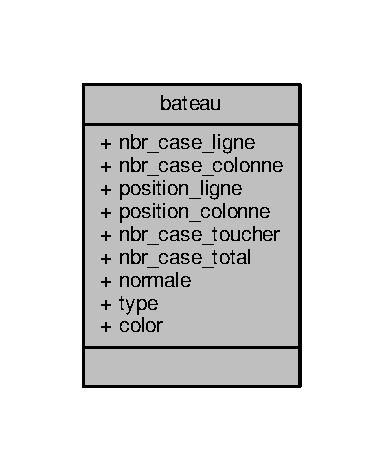
\includegraphics[width=184pt]{structbateau__coll__graph}
\end{center}
\end{figure}
\subsection*{Champs de données}
\begin{DoxyCompactItemize}
\item 
char \mbox{\hyperlink{structbateau_a5f7637b2932717e5589e1a368dd1b47b}{nbr\+\_\+case\+\_\+ligne}}
\item 
char \mbox{\hyperlink{structbateau_a1a56dd379e7c5cfc5714fd204947a0a8}{nbr\+\_\+case\+\_\+colonne}}
\item 
char \mbox{\hyperlink{structbateau_a5dcd33e534b9b1b8b0414325bc5c09b1}{position\+\_\+ligne}}
\item 
char \mbox{\hyperlink{structbateau_aac775edde7cde57176e580c29f6e8eca}{position\+\_\+colonne}}
\item 
char \mbox{\hyperlink{structbateau_a62ae80832c521a9984c520fde88dadfd}{nbr\+\_\+case\+\_\+toucher}}
\item 
char \mbox{\hyperlink{structbateau_aff445dc58a52069759f1e4bfd13c0313}{nbr\+\_\+case\+\_\+total}}
\item 
int \mbox{\hyperlink{structbateau_a77fe0bf7801ff08bf9b17e6c6237692e}{normale}}
\item 
int \mbox{\hyperlink{structbateau_ac4078d21fa180ff7d5c7e7fbf8a4a773}{type}}
\item 
char $\ast$ \mbox{\hyperlink{structbateau_a41910d4781ab6f3256d23f62b98c49a1}{color}}
\end{DoxyCompactItemize}


\subsection{Description détaillée}
Structure qui représente un bateau. 

Définition à la ligne 26 du fichier header.\+h.



\subsection{Documentation des champs}
\mbox{\Hypertarget{structbateau_a41910d4781ab6f3256d23f62b98c49a1}\label{structbateau_a41910d4781ab6f3256d23f62b98c49a1}} 
\index{bateau@{bateau}!color@{color}}
\index{color@{color}!bateau@{bateau}}
\subsubsection{\texorpdfstring{color}{color}}
{\footnotesize\ttfamily char$\ast$ bateau\+::color}

Variable indiquant la couleur du bateau 

Définition à la ligne 35 du fichier header.\+h.



Référencé par compar(), et positionement\+Des\+Bateaux().

\mbox{\Hypertarget{structbateau_a1a56dd379e7c5cfc5714fd204947a0a8}\label{structbateau_a1a56dd379e7c5cfc5714fd204947a0a8}} 
\index{bateau@{bateau}!nbr\+\_\+case\+\_\+colonne@{nbr\+\_\+case\+\_\+colonne}}
\index{nbr\+\_\+case\+\_\+colonne@{nbr\+\_\+case\+\_\+colonne}!bateau@{bateau}}
\subsubsection{\texorpdfstring{nbr\+\_\+case\+\_\+colonne}{nbr\_case\_colonne}}
{\footnotesize\ttfamily char bateau\+::nbr\+\_\+case\+\_\+colonne}

Variable indiquant le nombre de cases par colonne 

Définition à la ligne 28 du fichier header.\+h.



Référencé par compar(), positionement\+Des\+Bateaux(), et tour().

\mbox{\Hypertarget{structbateau_a5f7637b2932717e5589e1a368dd1b47b}\label{structbateau_a5f7637b2932717e5589e1a368dd1b47b}} 
\index{bateau@{bateau}!nbr\+\_\+case\+\_\+ligne@{nbr\+\_\+case\+\_\+ligne}}
\index{nbr\+\_\+case\+\_\+ligne@{nbr\+\_\+case\+\_\+ligne}!bateau@{bateau}}
\subsubsection{\texorpdfstring{nbr\+\_\+case\+\_\+ligne}{nbr\_case\_ligne}}
{\footnotesize\ttfamily char bateau\+::nbr\+\_\+case\+\_\+ligne}

Variable indiquant le nomre de cases par ligne 

Définition à la ligne 27 du fichier header.\+h.



Référencé par compar(), positionement\+Des\+Bateaux(), et tour().

\mbox{\Hypertarget{structbateau_aff445dc58a52069759f1e4bfd13c0313}\label{structbateau_aff445dc58a52069759f1e4bfd13c0313}} 
\index{bateau@{bateau}!nbr\+\_\+case\+\_\+total@{nbr\+\_\+case\+\_\+total}}
\index{nbr\+\_\+case\+\_\+total@{nbr\+\_\+case\+\_\+total}!bateau@{bateau}}
\subsubsection{\texorpdfstring{nbr\+\_\+case\+\_\+total}{nbr\_case\_total}}
{\footnotesize\ttfamily char bateau\+::nbr\+\_\+case\+\_\+total}

Variable indiquant le nombre de case total 

Définition à la ligne 32 du fichier header.\+h.



Référencé par compar(), positionement\+Des\+Bateaux(), et table\+Board().

\mbox{\Hypertarget{structbateau_a62ae80832c521a9984c520fde88dadfd}\label{structbateau_a62ae80832c521a9984c520fde88dadfd}} 
\index{bateau@{bateau}!nbr\+\_\+case\+\_\+toucher@{nbr\+\_\+case\+\_\+toucher}}
\index{nbr\+\_\+case\+\_\+toucher@{nbr\+\_\+case\+\_\+toucher}!bateau@{bateau}}
\subsubsection{\texorpdfstring{nbr\+\_\+case\+\_\+toucher}{nbr\_case\_toucher}}
{\footnotesize\ttfamily char bateau\+::nbr\+\_\+case\+\_\+toucher}

Variable indiquant le nombre de case toucher 

Définition à la ligne 31 du fichier header.\+h.



Référencé par compar(), positionement\+Des\+Bateaux(), table\+Board(), et tour().

\mbox{\Hypertarget{structbateau_a77fe0bf7801ff08bf9b17e6c6237692e}\label{structbateau_a77fe0bf7801ff08bf9b17e6c6237692e}} 
\index{bateau@{bateau}!normale@{normale}}
\index{normale@{normale}!bateau@{bateau}}
\subsubsection{\texorpdfstring{normale}{normale}}
{\footnotesize\ttfamily int bateau\+::normale}

Variable indiquant le nature du bateau 

Définition à la ligne 33 du fichier header.\+h.



Référencé par positionement\+Des\+Bateaux().

\mbox{\Hypertarget{structbateau_aac775edde7cde57176e580c29f6e8eca}\label{structbateau_aac775edde7cde57176e580c29f6e8eca}} 
\index{bateau@{bateau}!position\+\_\+colonne@{position\+\_\+colonne}}
\index{position\+\_\+colonne@{position\+\_\+colonne}!bateau@{bateau}}
\subsubsection{\texorpdfstring{position\+\_\+colonne}{position\_colonne}}
{\footnotesize\ttfamily char bateau\+::position\+\_\+colonne}

Variable indiquant la colonne exacte du bateau 

Définition à la ligne 30 du fichier header.\+h.



Référencé par compar(), positionement\+Des\+Bateaux(), et tour().

\mbox{\Hypertarget{structbateau_a5dcd33e534b9b1b8b0414325bc5c09b1}\label{structbateau_a5dcd33e534b9b1b8b0414325bc5c09b1}} 
\index{bateau@{bateau}!position\+\_\+ligne@{position\+\_\+ligne}}
\index{position\+\_\+ligne@{position\+\_\+ligne}!bateau@{bateau}}
\subsubsection{\texorpdfstring{position\+\_\+ligne}{position\_ligne}}
{\footnotesize\ttfamily char bateau\+::position\+\_\+ligne}

Variable indiquant la ligne exacte du bateau 

Définition à la ligne 29 du fichier header.\+h.



Référencé par compar(), positionement\+Des\+Bateaux(), et tour().

\mbox{\Hypertarget{structbateau_ac4078d21fa180ff7d5c7e7fbf8a4a773}\label{structbateau_ac4078d21fa180ff7d5c7e7fbf8a4a773}} 
\index{bateau@{bateau}!type@{type}}
\index{type@{type}!bateau@{bateau}}
\subsubsection{\texorpdfstring{type}{type}}
{\footnotesize\ttfamily int bateau\+::type}

Variable indiquant le type du bateau 

Définition à la ligne 34 du fichier header.\+h.



Référencé par positionement\+Des\+Bateaux().



La documentation de cette structure a été générée à partir du fichier suivant \+:\begin{DoxyCompactItemize}
\item 
\mbox{\hyperlink{header_8h}{header.\+h}}\end{DoxyCompactItemize}

\hypertarget{structjoueur}{}\section{Référence de la structure joueur}
\label{structjoueur}\index{joueur@{joueur}}


Structure qui représente un joueur.  




{\ttfamily \#include $<$header.\+h$>$}



Graphe de collaboration de joueur\+:\nopagebreak
\begin{figure}[H]
\begin{center}
\leavevmode
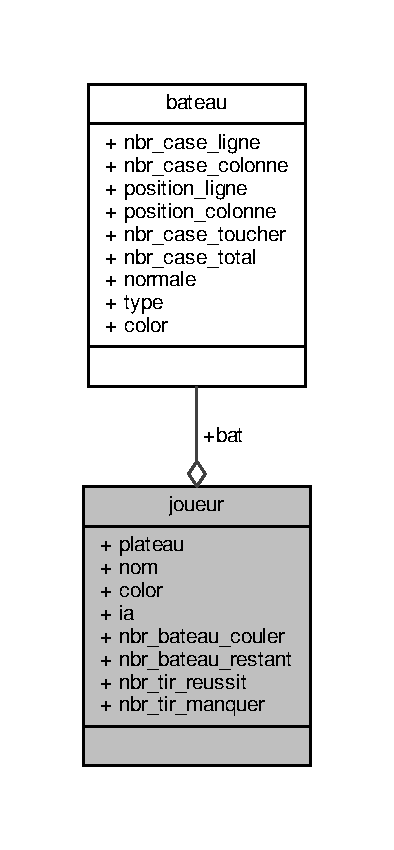
\includegraphics[width=189pt]{structjoueur__coll__graph}
\end{center}
\end{figure}
\subsection*{Champs de données}
\begin{DoxyCompactItemize}
\item 
char \mbox{\hyperlink{structjoueur_a0de66c3578a57ff8e0ed1bf3d91c8e82}{plateau}} \mbox{[}\mbox{\hyperlink{header_8h_adc3c2556e84bebbe78c8a87fc459a6f8}{T\+A\+I\+L\+L\+E\+\_\+\+P\+L\+A\+T\+E\+AU}}\mbox{]}\mbox{[}\mbox{\hyperlink{header_8h_adc3c2556e84bebbe78c8a87fc459a6f8}{T\+A\+I\+L\+L\+E\+\_\+\+P\+L\+A\+T\+E\+AU}}\mbox{]}
\item 
char $\ast$ \mbox{\hyperlink{structjoueur_a5228c842828b2639253cb7db01e6f72d}{nom}}
\item 
char $\ast$ \mbox{\hyperlink{structjoueur_a1064ba94d4d2719446f3c609135ba362}{color}}
\item 
int \mbox{\hyperlink{structjoueur_a307e3b4b4c1b78e753c599bc1f6a47c3}{ia}}
\item 
\mbox{\hyperlink{structbateau}{bateau}} \mbox{\hyperlink{structjoueur_a3b21aa14ce27f69126dc9a649b363146}{bat}} \mbox{[}10\mbox{]}
\item 
char \mbox{\hyperlink{structjoueur_ab0c0fa544d83148d4daed41c84954e55}{nbr\+\_\+bateau\+\_\+couler}}
\item 
char \mbox{\hyperlink{structjoueur_a4f902c486f8d66cb85cf3b07abd0bd12}{nbr\+\_\+bateau\+\_\+restant}}
\item 
char \mbox{\hyperlink{structjoueur_a19510a02b4ff3f6336da487b50806d71}{nbr\+\_\+tir\+\_\+reussit}}
\item 
int \mbox{\hyperlink{structjoueur_aaba095a23d03a15d363924e77caa3c1e}{nbr\+\_\+tir\+\_\+manquer}}
\end{DoxyCompactItemize}


\subsection{Description détaillée}
Structure qui représente un joueur. 

Définition à la ligne 40 du fichier header.\+h.



\subsection{Documentation des champs}
\mbox{\Hypertarget{structjoueur_a3b21aa14ce27f69126dc9a649b363146}\label{structjoueur_a3b21aa14ce27f69126dc9a649b363146}} 
\index{joueur@{joueur}!bat@{bat}}
\index{bat@{bat}!joueur@{joueur}}
\subsubsection{\texorpdfstring{bat}{bat}}
{\footnotesize\ttfamily \mbox{\hyperlink{structbateau}{bateau}} joueur\+::bat\mbox{[}10\mbox{]}}

Tableau de bateau 

Définition à la ligne 45 du fichier header.\+h.



Référencé par compar(), positionement\+Des\+Bateaux(), table\+Board(), et tour().

\mbox{\Hypertarget{structjoueur_a1064ba94d4d2719446f3c609135ba362}\label{structjoueur_a1064ba94d4d2719446f3c609135ba362}} 
\index{joueur@{joueur}!color@{color}}
\index{color@{color}!joueur@{joueur}}
\subsubsection{\texorpdfstring{color}{color}}
{\footnotesize\ttfamily char$\ast$ joueur\+::color}

Variable indiquant la color du joueur 

Définition à la ligne 43 du fichier header.\+h.



Référencé par afficher(), initialisation(), et print().

\mbox{\Hypertarget{structjoueur_a307e3b4b4c1b78e753c599bc1f6a47c3}\label{structjoueur_a307e3b4b4c1b78e753c599bc1f6a47c3}} 
\index{joueur@{joueur}!ia@{ia}}
\index{ia@{ia}!joueur@{joueur}}
\subsubsection{\texorpdfstring{ia}{ia}}
{\footnotesize\ttfamily int joueur\+::ia}

Variable indiquant la nature de joueur IA ou humain 

Définition à la ligne 44 du fichier header.\+h.



Référencé par initialisation(), jeu(), jeu\+A\+N\+Coup(), et tour().

\mbox{\Hypertarget{structjoueur_ab0c0fa544d83148d4daed41c84954e55}\label{structjoueur_ab0c0fa544d83148d4daed41c84954e55}} 
\index{joueur@{joueur}!nbr\+\_\+bateau\+\_\+couler@{nbr\+\_\+bateau\+\_\+couler}}
\index{nbr\+\_\+bateau\+\_\+couler@{nbr\+\_\+bateau\+\_\+couler}!joueur@{joueur}}
\subsubsection{\texorpdfstring{nbr\+\_\+bateau\+\_\+couler}{nbr\_bateau\_couler}}
{\footnotesize\ttfamily char joueur\+::nbr\+\_\+bateau\+\_\+couler}

Variable indiquant le nombre bateau couler 

Définition à la ligne 47 du fichier header.\+h.



Référencé par initialisation(), et table\+Board().

\mbox{\Hypertarget{structjoueur_a4f902c486f8d66cb85cf3b07abd0bd12}\label{structjoueur_a4f902c486f8d66cb85cf3b07abd0bd12}} 
\index{joueur@{joueur}!nbr\+\_\+bateau\+\_\+restant@{nbr\+\_\+bateau\+\_\+restant}}
\index{nbr\+\_\+bateau\+\_\+restant@{nbr\+\_\+bateau\+\_\+restant}!joueur@{joueur}}
\subsubsection{\texorpdfstring{nbr\+\_\+bateau\+\_\+restant}{nbr\_bateau\_restant}}
{\footnotesize\ttfamily char joueur\+::nbr\+\_\+bateau\+\_\+restant}

Variable indiquant le nombre bateau restant 

Définition à la ligne 48 du fichier header.\+h.



Référencé par initialisation(), et table\+Board().

\mbox{\Hypertarget{structjoueur_aaba095a23d03a15d363924e77caa3c1e}\label{structjoueur_aaba095a23d03a15d363924e77caa3c1e}} 
\index{joueur@{joueur}!nbr\+\_\+tir\+\_\+manquer@{nbr\+\_\+tir\+\_\+manquer}}
\index{nbr\+\_\+tir\+\_\+manquer@{nbr\+\_\+tir\+\_\+manquer}!joueur@{joueur}}
\subsubsection{\texorpdfstring{nbr\+\_\+tir\+\_\+manquer}{nbr\_tir\_manquer}}
{\footnotesize\ttfamily int joueur\+::nbr\+\_\+tir\+\_\+manquer}

Variable indiquant le nombre de tirs manqués 

Définition à la ligne 50 du fichier header.\+h.



Référencé par initialisation(), table\+Board(), et tour().

\mbox{\Hypertarget{structjoueur_a19510a02b4ff3f6336da487b50806d71}\label{structjoueur_a19510a02b4ff3f6336da487b50806d71}} 
\index{joueur@{joueur}!nbr\+\_\+tir\+\_\+reussit@{nbr\+\_\+tir\+\_\+reussit}}
\index{nbr\+\_\+tir\+\_\+reussit@{nbr\+\_\+tir\+\_\+reussit}!joueur@{joueur}}
\subsubsection{\texorpdfstring{nbr\+\_\+tir\+\_\+reussit}{nbr\_tir\_reussit}}
{\footnotesize\ttfamily char joueur\+::nbr\+\_\+tir\+\_\+reussit}

Variable indiquant le nombre de tirs réussis 

Définition à la ligne 49 du fichier header.\+h.



Référencé par game\+Over(), initialisation(), table\+Board(), et tour().

\mbox{\Hypertarget{structjoueur_a5228c842828b2639253cb7db01e6f72d}\label{structjoueur_a5228c842828b2639253cb7db01e6f72d}} 
\index{joueur@{joueur}!nom@{nom}}
\index{nom@{nom}!joueur@{joueur}}
\subsubsection{\texorpdfstring{nom}{nom}}
{\footnotesize\ttfamily char$\ast$ joueur\+::nom}

Variable indiquant le nom du joueur 

Définition à la ligne 42 du fichier header.\+h.



Référencé par afficher(), initialisation(), et print().

\mbox{\Hypertarget{structjoueur_a0de66c3578a57ff8e0ed1bf3d91c8e82}\label{structjoueur_a0de66c3578a57ff8e0ed1bf3d91c8e82}} 
\index{joueur@{joueur}!plateau@{plateau}}
\index{plateau@{plateau}!joueur@{joueur}}
\subsubsection{\texorpdfstring{plateau}{plateau}}
{\footnotesize\ttfamily char joueur\+::plateau\mbox{[}\mbox{\hyperlink{header_8h_adc3c2556e84bebbe78c8a87fc459a6f8}{T\+A\+I\+L\+L\+E\+\_\+\+P\+L\+A\+T\+E\+AU}}\mbox{]}\mbox{[}\mbox{\hyperlink{header_8h_adc3c2556e84bebbe78c8a87fc459a6f8}{T\+A\+I\+L\+L\+E\+\_\+\+P\+L\+A\+T\+E\+AU}}\mbox{]}}



Définition à la ligne 41 du fichier header.\+h.



Référencé par afficher(), initialisation(), positionement\+Des\+Bateaux(), et tour().



La documentation de cette structure a été générée à partir du fichier suivant \+:\begin{DoxyCompactItemize}
\item 
\mbox{\hyperlink{header_8h}{header.\+h}}\end{DoxyCompactItemize}

\chapter{Documentation des fichiers}
\hypertarget{affichage_8c}{}\section{Référence du fichier affichage.\+c}
\label{affichage_8c}\index{affichage.\+c@{affichage.\+c}}
{\ttfamily \#include \char`\"{}header.\+h\char`\"{}}\newline
Graphe des dépendances par inclusion de affichage.\+c\+:\nopagebreak
\begin{figure}[H]
\begin{center}
\leavevmode
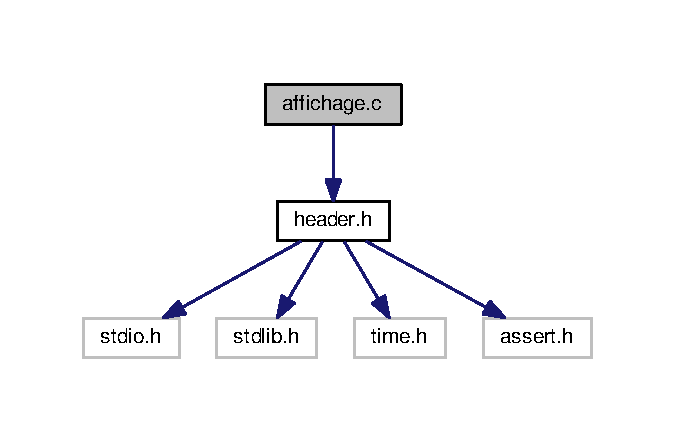
\includegraphics[width=324pt]{affichage_8c__incl}
\end{center}
\end{figure}
\subsection*{Fonctions}
\begin{DoxyCompactItemize}
\item 
void \mbox{\hyperlink{affichage_8c_a8004c5a076f6d53e90583b921ac810cb}{afficher}} (\mbox{\hyperlink{structjoueur}{joueur}} $\ast$joueur1, \mbox{\hyperlink{structjoueur}{joueur}} $\ast$joueur2, int cacher)
\begin{DoxyCompactList}\small\item\em Une fonction qui affiche le plateau de jeu. \end{DoxyCompactList}\item 
void \mbox{\hyperlink{affichage_8c_a34b6e28e00a180632a300b9608ad6acd}{print}} (\mbox{\hyperlink{structjoueur}{joueur}} $\ast$player, int c)
\begin{DoxyCompactList}\small\item\em Une fonction qui affiche différent messager de mise en forme dasn le jeu a l\textquotesingle{}aide d\textquotesingle{}un int donner comme argument. \end{DoxyCompactList}\item 
void \mbox{\hyperlink{affichage_8c_a671ab408369ac69a9b4d3afc29c6fd21}{table\+Board}} (\mbox{\hyperlink{structjoueur}{joueur}} $\ast$player)
\begin{DoxyCompactList}\small\item\em Une fonction qui affiche le resultat du joueur actuelle à chaque tour. \end{DoxyCompactList}\item 
void \mbox{\hyperlink{affichage_8c_adba405b6c8341bbae8459669db1aa775}{compar}} (int ligne, int colonne, \mbox{\hyperlink{structjoueur}{joueur}} $\ast$player, int choix, char $\ast$$\ast$\mbox{\hyperlink{header_8h_aabcb2d6536b6c0ab41f99493c911489b}{couleur}})
\begin{DoxyCompactList}\small\item\em Une fonction qui récupere une couleur selon des conditions. \end{DoxyCompactList}\end{DoxyCompactItemize}


\subsection{Description détaillée}
\begin{DoxyAuthor}{Auteur}
B.\+Habib, A.\+Sofiane, I.\+Tinhinane, I.\+Chafia 
\end{DoxyAuthor}
\begin{DoxyVersion}{Version}
1.\+0 
\end{DoxyVersion}
\begin{DoxyDate}{Date}
07 Avril 2018
\end{DoxyDate}
définition de tous les fonction d\textquotesingle{}affichage 

\subsection{Documentation des fonctions}
\mbox{\Hypertarget{affichage_8c_a8004c5a076f6d53e90583b921ac810cb}\label{affichage_8c_a8004c5a076f6d53e90583b921ac810cb}} 
\index{affichage.\+c@{affichage.\+c}!afficher@{afficher}}
\index{afficher@{afficher}!affichage.\+c@{affichage.\+c}}
\subsubsection{\texorpdfstring{afficher()}{afficher()}}
{\footnotesize\ttfamily void afficher (\begin{DoxyParamCaption}\item[{\mbox{\hyperlink{structjoueur}{joueur}} $\ast$}]{joueur1,  }\item[{\mbox{\hyperlink{structjoueur}{joueur}} $\ast$}]{joueur2,  }\item[{int}]{cacher }\end{DoxyParamCaption})}



Une fonction qui affiche le plateau de jeu. 

Cette fonction permet d\textquotesingle{}afficher tous le contenu du plateau les deux grilles des deux joueur une grille cacher du joueur adversaire et l\textquotesingle{}autre afficher normale celle du joueur actuelle. 
\begin{DoxyParams}{Paramètres}
{\em joueur$\ast$} & joueur1 \+: le joueur adversaire. \\
\hline
{\em joueur$\ast$} & joueur2 \+: le joueur actuelle. \\
\hline
{\em int} & cacher \+: une variable qui nous dit a ce que en fait un affichage cacher ou pas. \\
\hline
\end{DoxyParams}


Définition à la ligne 10 du fichier affichage.\+c.



Références joueur\+::color, compar(), couleur, joueur\+::nom, joueur\+::plateau, R\+ED, table\+Board(), T\+A\+I\+L\+L\+E\+\_\+\+P\+L\+A\+T\+E\+AU, et W\+H\+I\+TE.



Référencé par jeu(), et jeu\+A\+N\+Coup().


\begin{DoxyCode}
10                                                            \{
11     \textcolor{keywordtype}{int} ligne, colonne, i;
12     \textcolor{keywordtype}{char}* \mbox{\hyperlink{header_8h_aabcb2d6536b6c0ab41f99493c911489b}{couleur}};
13     \mbox{\hyperlink{affichage_8c_a671ab408369ac69a9b4d3afc29c6fd21}{tableBoard}}(joueur2); \textcolor{comment}{// lLa fonction qui affiche des informations sur le resultat du jeu pour
       chaque joueur }
14     \mbox{\hyperlink{header_8h_aabcb2d6536b6c0ab41f99493c911489b}{couleur}}(\textcolor{stringliteral}{"47"});\mbox{\hyperlink{header_8h_aabcb2d6536b6c0ab41f99493c911489b}{couleur}}(\mbox{\hyperlink{header_8h_a8d23feea868a983c8c2b661e1e16972f}{RED}});printf(\textcolor{stringliteral}{"\(\backslash\)t\(\backslash\)t  Plateau du joueur \%s  "},joueur1->
      \mbox{\hyperlink{structjoueur_a5228c842828b2639253cb7db01e6f72d}{nom}});\mbox{\hyperlink{header_8h_aabcb2d6536b6c0ab41f99493c911489b}{couleur}}(\mbox{\hyperlink{header_8h_a87b537f5fa5c109d3c05c13d6b18f382}{WHITE}});
15     \mbox{\hyperlink{header_8h_aabcb2d6536b6c0ab41f99493c911489b}{couleur}}(\textcolor{stringliteral}{"47"});\mbox{\hyperlink{header_8h_aabcb2d6536b6c0ab41f99493c911489b}{couleur}}(\mbox{\hyperlink{header_8h_a8d23feea868a983c8c2b661e1e16972f}{RED}});printf(\textcolor{stringliteral}{"\(\backslash\)t\(\backslash\)t\(\backslash\)t\(\backslash\)t\(\backslash\)t\(\backslash\)t\(\backslash\)t  Mon Plateau  \%s \(\backslash\)n"},joueur2->
      \mbox{\hyperlink{structjoueur_a5228c842828b2639253cb7db01e6f72d}{nom}});\mbox{\hyperlink{header_8h_aabcb2d6536b6c0ab41f99493c911489b}{couleur}}(\mbox{\hyperlink{header_8h_a87b537f5fa5c109d3c05c13d6b18f382}{WHITE}});
16     \textcolor{comment}{// Afficher les numeros de colonne pour la grille de l'adversaire  (player 1)}
17     \textcolor{keywordflow}{for}(colonne = 1 ; colonne <= \mbox{\hyperlink{header_8h_adc3c2556e84bebbe78c8a87fc459a6f8}{TAILLE\_PLATEAU}} ; ++colonne)
18         \textcolor{keywordflow}{if}(colonne < 10)
19             printf(\textcolor{stringliteral}{"  \%d "},colonne);
20         \textcolor{keywordflow}{else}
21             printf(\textcolor{stringliteral}{" \%d "},colonne);
22     printf(\textcolor{stringliteral}{"      "});
23     \textcolor{comment}{// Afficher les numeros de colonne pour la grille de jouer actuelle (player 2)}
24     \textcolor{keywordflow}{for}(colonne = 1 ; colonne <= \mbox{\hyperlink{header_8h_adc3c2556e84bebbe78c8a87fc459a6f8}{TAILLE\_PLATEAU}} ; ++colonne)
25         \textcolor{keywordflow}{if}(colonne < 10)
26             printf(\textcolor{stringliteral}{"  \%d "},colonne);
27         \textcolor{keywordflow}{else}
28             printf(\textcolor{stringliteral}{" \%d "},colonne);
29     printf(\textcolor{stringliteral}{"\(\backslash\)n"});
30 
31     \textcolor{keywordflow}{for}(ligne = 0 ; ligne < \mbox{\hyperlink{header_8h_adc3c2556e84bebbe78c8a87fc459a6f8}{TAILLE\_PLATEAU}} ; ++ligne)\{
32         printf(\textcolor{stringliteral}{"-"});
33         \textcolor{keywordflow}{for}(i = 0 ; i < \mbox{\hyperlink{header_8h_adc3c2556e84bebbe78c8a87fc459a6f8}{TAILLE\_PLATEAU}}; i++)  
34             printf(\textcolor{stringliteral}{"----"});
35         printf(\textcolor{stringliteral}{"     "});
36         printf(\textcolor{stringliteral}{"-"});
37         \textcolor{keywordflow}{for}(i = 0 ; i < \mbox{\hyperlink{header_8h_adc3c2556e84bebbe78c8a87fc459a6f8}{TAILLE\_PLATEAU}}; i++)  
38             printf(\textcolor{stringliteral}{"----"});
39         printf(\textcolor{stringliteral}{"\(\backslash\)n"});
40         \textcolor{comment}{// Afficher la grille de l'adversaire (joueur1) en cachent les bateaux non toucher }
41         \textcolor{keywordflow}{for}(colonne = 0 ; colonne < \mbox{\hyperlink{header_8h_adc3c2556e84bebbe78c8a87fc459a6f8}{TAILLE\_PLATEAU}} ; ++colonne)
42                 \textcolor{keywordflow}{if}(joueur1->\mbox{\hyperlink{structjoueur_a0de66c3578a57ff8e0ed1bf3d91c8e82}{plateau}}[ligne][colonne] == \textcolor{charliteral}{'\#'} \&\& cacher == 1)
43                     printf(\textcolor{stringliteral}{"|   "});
44                 \textcolor{keywordflow}{else} \textcolor{keywordflow}{if}(joueur1->\mbox{\hyperlink{structjoueur_a0de66c3578a57ff8e0ed1bf3d91c8e82}{plateau}}[ligne][colonne] == \textcolor{charliteral}{'X'})\{
45                     printf(\textcolor{stringliteral}{"| "});
46                     \mbox{\hyperlink{header_8h_aabcb2d6536b6c0ab41f99493c911489b}{couleur}} = \mbox{\hyperlink{header_8h_a8d23feea868a983c8c2b661e1e16972f}{RED}};
47                     \mbox{\hyperlink{affichage_8c_adba405b6c8341bbae8459669db1aa775}{compar}}(ligne, colonne, joueur1, 1, \&\mbox{\hyperlink{header_8h_aabcb2d6536b6c0ab41f99493c911489b}{couleur}});
48                     \mbox{\hyperlink{header_8h_aabcb2d6536b6c0ab41f99493c911489b}{couleur}}(\mbox{\hyperlink{header_8h_aabcb2d6536b6c0ab41f99493c911489b}{couleur}});
49                     printf(\textcolor{stringliteral}{"\%c "},joueur1->\mbox{\hyperlink{structjoueur_a0de66c3578a57ff8e0ed1bf3d91c8e82}{plateau}}[ligne][colonne]);
50                     \mbox{\hyperlink{header_8h_aabcb2d6536b6c0ab41f99493c911489b}{couleur}}(\mbox{\hyperlink{header_8h_a87b537f5fa5c109d3c05c13d6b18f382}{WHITE}});
51                 \}\textcolor{keywordflow}{else}\{
52                     printf(\textcolor{stringliteral}{"| "});
53                     \mbox{\hyperlink{header_8h_aabcb2d6536b6c0ab41f99493c911489b}{couleur}}(joueur1->\mbox{\hyperlink{structjoueur_a1064ba94d4d2719446f3c609135ba362}{color}});
54                     printf(\textcolor{stringliteral}{"\%c "},joueur1->\mbox{\hyperlink{structjoueur_a0de66c3578a57ff8e0ed1bf3d91c8e82}{plateau}}[ligne][colonne]);
55                     \mbox{\hyperlink{header_8h_aabcb2d6536b6c0ab41f99493c911489b}{couleur}}(\mbox{\hyperlink{header_8h_a87b537f5fa5c109d3c05c13d6b18f382}{WHITE}});
56                 \}
57         
58         \textcolor{keywordflow}{if}(ligne + 1 < 10)
59             printf(\textcolor{stringliteral}{"|  \%d  "}, ligne + 1);
60         \textcolor{keywordflow}{else}
61             printf(\textcolor{stringliteral}{"|  \%d "}, ligne + 1);
62         \textcolor{comment}{// Afficher la grille du joueur acctuelle (joueur2)  }
63         \textcolor{keywordflow}{for}(colonne = 0 ; colonne < \mbox{\hyperlink{header_8h_adc3c2556e84bebbe78c8a87fc459a6f8}{TAILLE\_PLATEAU}} ; ++colonne)
64                 \textcolor{keywordflow}{if}(joueur2->\mbox{\hyperlink{structjoueur_a0de66c3578a57ff8e0ed1bf3d91c8e82}{plateau}}[ligne][colonne] == \textcolor{charliteral}{'O'})
65                     printf(\textcolor{stringliteral}{"|   "});
66                 \textcolor{keywordflow}{else} \textcolor{keywordflow}{if}(joueur2->\mbox{\hyperlink{structjoueur_a0de66c3578a57ff8e0ed1bf3d91c8e82}{plateau}}[ligne][colonne] == \textcolor{charliteral}{'X'})\{
67                     \mbox{\hyperlink{header_8h_aabcb2d6536b6c0ab41f99493c911489b}{couleur}} = \mbox{\hyperlink{header_8h_a8d23feea868a983c8c2b661e1e16972f}{RED}};
68                     \mbox{\hyperlink{affichage_8c_adba405b6c8341bbae8459669db1aa775}{compar}}(ligne, colonne, joueur2, 1, \&\mbox{\hyperlink{header_8h_aabcb2d6536b6c0ab41f99493c911489b}{couleur}});
69                     printf(\textcolor{stringliteral}{"| "});
70                     \mbox{\hyperlink{header_8h_aabcb2d6536b6c0ab41f99493c911489b}{couleur}}(\mbox{\hyperlink{header_8h_aabcb2d6536b6c0ab41f99493c911489b}{couleur}});
71                     printf(\textcolor{stringliteral}{"\%c "},joueur2->\mbox{\hyperlink{structjoueur_a0de66c3578a57ff8e0ed1bf3d91c8e82}{plateau}}[ligne][colonne]);
72                     \mbox{\hyperlink{header_8h_aabcb2d6536b6c0ab41f99493c911489b}{couleur}}(\mbox{\hyperlink{header_8h_a87b537f5fa5c109d3c05c13d6b18f382}{WHITE}});
73                 \}\textcolor{keywordflow}{else}\{
74                     \mbox{\hyperlink{header_8h_aabcb2d6536b6c0ab41f99493c911489b}{couleur}} = joueur2->\mbox{\hyperlink{structjoueur_a1064ba94d4d2719446f3c609135ba362}{color}};
75                     \mbox{\hyperlink{affichage_8c_adba405b6c8341bbae8459669db1aa775}{compar}}(ligne, colonne, joueur2, 0, \&\mbox{\hyperlink{header_8h_aabcb2d6536b6c0ab41f99493c911489b}{couleur}});
76                     printf(\textcolor{stringliteral}{"| "});
77                     \mbox{\hyperlink{header_8h_aabcb2d6536b6c0ab41f99493c911489b}{couleur}}(\mbox{\hyperlink{header_8h_aabcb2d6536b6c0ab41f99493c911489b}{couleur}});
78                     printf(\textcolor{stringliteral}{"\%c "},joueur2->\mbox{\hyperlink{structjoueur_a0de66c3578a57ff8e0ed1bf3d91c8e82}{plateau}}[ligne][colonne]);
79                     \mbox{\hyperlink{header_8h_aabcb2d6536b6c0ab41f99493c911489b}{couleur}}(\mbox{\hyperlink{header_8h_a87b537f5fa5c109d3c05c13d6b18f382}{WHITE}});
80                 \}
81         printf(\textcolor{stringliteral}{"|\(\backslash\)n"});
82     \}
83  
84     printf(\textcolor{stringliteral}{"-"});
85     \textcolor{keywordflow}{for}(i = 0 ; i < \mbox{\hyperlink{header_8h_adc3c2556e84bebbe78c8a87fc459a6f8}{TAILLE\_PLATEAU}}; i++)  
86         printf(\textcolor{stringliteral}{"----"});
87     printf(\textcolor{stringliteral}{"     "});
88     printf(\textcolor{stringliteral}{"-"});
89     \textcolor{keywordflow}{for}(i = 0 ; i < \mbox{\hyperlink{header_8h_adc3c2556e84bebbe78c8a87fc459a6f8}{TAILLE\_PLATEAU}}; i++)  
90         printf(\textcolor{stringliteral}{"----"});
91     printf(\textcolor{stringliteral}{"\(\backslash\)n"});
92 \}
\end{DoxyCode}
Voici le graphe d\textquotesingle{}appel pour cette fonction \+:\nopagebreak
\begin{figure}[H]
\begin{center}
\leavevmode
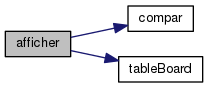
\includegraphics[width=228pt]{affichage_8c_a8004c5a076f6d53e90583b921ac810cb_cgraph}
\end{center}
\end{figure}
Voici le graphe des appelants de cette fonction \+:\nopagebreak
\begin{figure}[H]
\begin{center}
\leavevmode
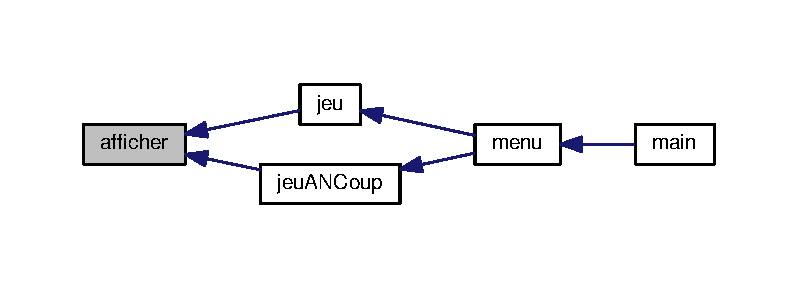
\includegraphics[width=350pt]{affichage_8c_a8004c5a076f6d53e90583b921ac810cb_icgraph}
\end{center}
\end{figure}
\mbox{\Hypertarget{affichage_8c_adba405b6c8341bbae8459669db1aa775}\label{affichage_8c_adba405b6c8341bbae8459669db1aa775}} 
\index{affichage.\+c@{affichage.\+c}!compar@{compar}}
\index{compar@{compar}!affichage.\+c@{affichage.\+c}}
\subsubsection{\texorpdfstring{compar()}{compar()}}
{\footnotesize\ttfamily void compar (\begin{DoxyParamCaption}\item[{int}]{ligne,  }\item[{int}]{colonne,  }\item[{\mbox{\hyperlink{structjoueur}{joueur}} $\ast$}]{player,  }\item[{int}]{choix,  }\item[{char $\ast$$\ast$}]{couleur }\end{DoxyParamCaption})}



Une fonction qui récupere une couleur selon des conditions. 

Cette fonction permet de récuperer soit la couleur real du bateau c\textquotesingle{}est choix==0, soit une autre couleur c\textquotesingle{}est tous le bateau est toucher 
\begin{DoxyParams}{Paramètres}
{\em int} & ligne \+: la ligne d\textquotesingle{}une case à tester. \\
\hline
{\em int} & colonne\+: la colonne d\textquotesingle{}une case à tester. \\
\hline
{\em joueur$\ast$} & player \+: le joueur actuelle. \\
\hline
{\em int} & choix \+: une variable qui nos sert à faire deux teste différent dans une fonction. \\
\hline
{\em char$\ast$$\ast$} & couleur \+: une pointeur sur la variable couleur. \\
\hline
\end{DoxyParams}


Définition à la ligne 152 du fichier affichage.\+c.



Références joueur\+::bat, bateau\+::color, couleur, bateau\+::nbr\+\_\+case\+\_\+colonne, bateau\+::nbr\+\_\+case\+\_\+ligne, bateau\+::nbr\+\_\+case\+\_\+total, bateau\+::nbr\+\_\+case\+\_\+toucher, N\+O\+M\+B\+R\+E\+\_\+\+B\+A\+T\+E\+AU, bateau\+::position\+\_\+colonne, et bateau\+::position\+\_\+ligne.



Référencé par afficher().


\begin{DoxyCode}
152                                                                               \{
153     \textcolor{keywordtype}{int} test, i;
154     \textcolor{keywordflow}{for} (i = 0; i < \mbox{\hyperlink{header_8h_a56aaacd8cb8ffd138094887b2d3344f6}{NOMBRE\_BATEAU}}; ++i)\{
155         test = ((colonne >= player->\mbox{\hyperlink{structjoueur_a3b21aa14ce27f69126dc9a649b363146}{bat}}[i].\mbox{\hyperlink{structbateau_aac775edde7cde57176e580c29f6e8eca}{position\_colonne}}) \&\& (colonne < player->
      \mbox{\hyperlink{structjoueur_a3b21aa14ce27f69126dc9a649b363146}{bat}}[i].position\_colonne + player->\mbox{\hyperlink{structjoueur_a3b21aa14ce27f69126dc9a649b363146}{bat}}[i].\mbox{\hyperlink{structbateau_a1a56dd379e7c5cfc5714fd204947a0a8}{nbr\_case\_colonne}})) 
156                 \&\&((ligne >= player->\mbox{\hyperlink{structjoueur_a3b21aa14ce27f69126dc9a649b363146}{bat}}[i].\mbox{\hyperlink{structbateau_a5dcd33e534b9b1b8b0414325bc5c09b1}{position\_ligne}}) \&\& (ligne < player->
      \mbox{\hyperlink{structjoueur_a3b21aa14ce27f69126dc9a649b363146}{bat}}[i].\mbox{\hyperlink{structbateau_a5dcd33e534b9b1b8b0414325bc5c09b1}{position\_ligne}} + player->\mbox{\hyperlink{structjoueur_a3b21aa14ce27f69126dc9a649b363146}{bat}}[i].\mbox{\hyperlink{structbateau_a5f7637b2932717e5589e1a368dd1b47b}{nbr\_case\_ligne}}));
157 
158         \textcolor{keywordflow}{if}(test \&\& (player->\mbox{\hyperlink{structjoueur_a3b21aa14ce27f69126dc9a649b363146}{bat}}[i].\mbox{\hyperlink{structbateau_aff445dc58a52069759f1e4bfd13c0313}{nbr\_case\_total}} == player->
      \mbox{\hyperlink{structjoueur_a3b21aa14ce27f69126dc9a649b363146}{bat}}[i].\mbox{\hyperlink{structbateau_a62ae80832c521a9984c520fde88dadfd}{nbr\_case\_toucher}}) \&\& (choix == 1))\{       
159             *\mbox{\hyperlink{header_8h_aabcb2d6536b6c0ab41f99493c911489b}{couleur}} = \textcolor{stringliteral}{"40"};
160             \textcolor{keywordflow}{break};
161         \}
162         \textcolor{keywordflow}{if}(test \&\& (choix == 0))\{
163             *\mbox{\hyperlink{header_8h_aabcb2d6536b6c0ab41f99493c911489b}{couleur}} = player->\mbox{\hyperlink{structjoueur_a3b21aa14ce27f69126dc9a649b363146}{bat}}[i].\mbox{\hyperlink{structbateau_a41910d4781ab6f3256d23f62b98c49a1}{color}};
164             \textcolor{keywordflow}{break};
165         \}
166     \}
167 \}
\end{DoxyCode}
Voici le graphe des appelants de cette fonction \+:\nopagebreak
\begin{figure}[H]
\begin{center}
\leavevmode
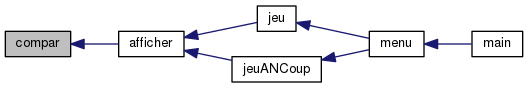
\includegraphics[width=350pt]{affichage_8c_adba405b6c8341bbae8459669db1aa775_icgraph}
\end{center}
\end{figure}
\mbox{\Hypertarget{affichage_8c_a34b6e28e00a180632a300b9608ad6acd}\label{affichage_8c_a34b6e28e00a180632a300b9608ad6acd}} 
\index{affichage.\+c@{affichage.\+c}!print@{print}}
\index{print@{print}!affichage.\+c@{affichage.\+c}}
\subsubsection{\texorpdfstring{print()}{print()}}
{\footnotesize\ttfamily void print (\begin{DoxyParamCaption}\item[{\mbox{\hyperlink{structjoueur}{joueur}} $\ast$}]{player,  }\item[{int}]{c }\end{DoxyParamCaption})}



Une fonction qui affiche différent messager de mise en forme dasn le jeu a l\textquotesingle{}aide d\textquotesingle{}un int donner comme argument. 

Cette fonction permet d\textquotesingle{}afficher plusieur message d\textquotesingle{}indication selon la valeur de \char`\"{}int c\char`\"{}. 
\begin{DoxyParams}{Paramètres}
{\em joueur$\ast$} & player \+: le joueur. \\
\hline
{\em int} & cacher \+: une variable qui prend les valeurs 0, 1 , 2 et 3 . \\
\hline
\end{DoxyParams}


Définition à la ligne 99 du fichier affichage.\+c.



Références joueur\+::color, couleur, joueur\+::nom, R\+ED, et W\+H\+I\+TE.



Référencé par game\+Over(), jeu(), et jeu\+A\+N\+Coup().


\begin{DoxyCode}
99                                  \{
100     fflush(stdin);
101     \textcolor{keywordflow}{if}(c == 0)\{
102         \mbox{\hyperlink{header_8h_aabcb2d6536b6c0ab41f99493c911489b}{couleur}}(\mbox{\hyperlink{header_8h_a8d23feea868a983c8c2b661e1e16972f}{RED}}); printf(\textcolor{stringliteral}{"\%s, appyer sur entreé pour continuer!!\(\backslash\)n"}, player->
      \mbox{\hyperlink{structjoueur_a5228c842828b2639253cb7db01e6f72d}{nom}});
103         \mbox{\hyperlink{header_8h_aabcb2d6536b6c0ab41f99493c911489b}{couleur}}(\mbox{\hyperlink{header_8h_a87b537f5fa5c109d3c05c13d6b18f382}{WHITE}});
104         getchar();
105        CLEAR\_SCREEN;
106     \}\textcolor{keywordflow}{else} \textcolor{keywordflow}{if}(c == 1)\{
107         \mbox{\hyperlink{header_8h_aabcb2d6536b6c0ab41f99493c911489b}{couleur}}(\textcolor{stringliteral}{"47"}); \mbox{\hyperlink{header_8h_aabcb2d6536b6c0ab41f99493c911489b}{couleur}}(\mbox{\hyperlink{header_8h_a8d23feea868a983c8c2b661e1e16972f}{RED}});printf(\textcolor{stringliteral}{"\%s"},player->\mbox{\hyperlink{structjoueur_a5228c842828b2639253cb7db01e6f72d}{nom}});
108         printf(\textcolor{stringliteral}{", c'est ton tour de joue:\(\backslash\)n---------------------------\(\backslash\)n"});
109         \mbox{\hyperlink{header_8h_aabcb2d6536b6c0ab41f99493c911489b}{couleur}}(\mbox{\hyperlink{header_8h_a87b537f5fa5c109d3c05c13d6b18f382}{WHITE}});     
110     \}\textcolor{keywordflow}{else} \textcolor{keywordflow}{if}(c == 2)\{
111         printf(\textcolor{stringliteral}{"Le joueur "});
112         \mbox{\hyperlink{header_8h_aabcb2d6536b6c0ab41f99493c911489b}{couleur}}(player->\mbox{\hyperlink{structjoueur_a1064ba94d4d2719446f3c609135ba362}{color}});printf(\textcolor{stringliteral}{"\%s "},player->\mbox{\hyperlink{structjoueur_a5228c842828b2639253cb7db01e6f72d}{nom}});
113         \mbox{\hyperlink{header_8h_aabcb2d6536b6c0ab41f99493c911489b}{couleur}}(\mbox{\hyperlink{header_8h_a87b537f5fa5c109d3c05c13d6b18f382}{WHITE}});printf(\textcolor{stringliteral}{"à Gagner ^-^.\(\backslash\)n"});       
114         printf(\textcolor{stringliteral}{"La partie est terminer.\(\backslash\)nAppyer sur entreé pour revenir au menu principal!!"});
115         getchar();
116         CLEAR\_SCREEN;
117     \}\textcolor{keywordflow}{else} \textcolor{keywordflow}{if}(c == 3)\{
118         printf(\textcolor{stringliteral}{"La partie Va Commencer.\(\backslash\)nAppyer sur entreé pour continuer!!"});
119         getchar();
120         CLEAR\_SCREEN;
121     \}
122 \}
\end{DoxyCode}
Voici le graphe des appelants de cette fonction \+:\nopagebreak
\begin{figure}[H]
\begin{center}
\leavevmode
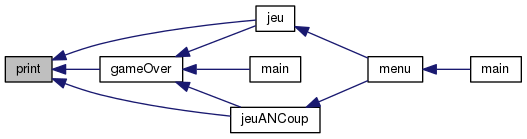
\includegraphics[width=350pt]{affichage_8c_a34b6e28e00a180632a300b9608ad6acd_icgraph}
\end{center}
\end{figure}
\mbox{\Hypertarget{affichage_8c_a671ab408369ac69a9b4d3afc29c6fd21}\label{affichage_8c_a671ab408369ac69a9b4d3afc29c6fd21}} 
\index{affichage.\+c@{affichage.\+c}!table\+Board@{table\+Board}}
\index{table\+Board@{table\+Board}!affichage.\+c@{affichage.\+c}}
\subsubsection{\texorpdfstring{table\+Board()}{tableBoard()}}
{\footnotesize\ttfamily void table\+Board (\begin{DoxyParamCaption}\item[{\mbox{\hyperlink{structjoueur}{joueur}} $\ast$}]{player }\end{DoxyParamCaption})}



Une fonction qui affiche le resultat du joueur actuelle à chaque tour. 

Cette fonction permet d\textquotesingle{}afficher les resultats de chaque joueur a chaque tour de jeu. ~\newline

\begin{DoxyParams}{Paramètres}
{\em joueur$\ast$} & player \+: le joueur. \\
\hline
\end{DoxyParams}


Définition à la ligne 128 du fichier affichage.\+c.



Références joueur\+::bat, couleur, joueur\+::nbr\+\_\+bateau\+\_\+couler, joueur\+::nbr\+\_\+bateau\+\_\+restant, bateau\+::nbr\+\_\+case\+\_\+total, bateau\+::nbr\+\_\+case\+\_\+toucher, joueur\+::nbr\+\_\+tir\+\_\+manquer, joueur\+::nbr\+\_\+tir\+\_\+reussit, N\+O\+M\+B\+R\+E\+\_\+\+B\+A\+T\+E\+AU, et W\+H\+I\+TE.



Référencé par afficher().


\begin{DoxyCode}
128                                \{
129     \textcolor{keywordtype}{int} i;
130     player->\mbox{\hyperlink{structjoueur_ab0c0fa544d83148d4daed41c84954e55}{nbr\_bateau\_couler}} = 0;
131     \textcolor{keywordflow}{for} (i = 0; i < \mbox{\hyperlink{header_8h_a56aaacd8cb8ffd138094887b2d3344f6}{NOMBRE\_BATEAU}}; ++i)\{
132         \textcolor{keywordflow}{if}(player->\mbox{\hyperlink{structjoueur_a3b21aa14ce27f69126dc9a649b363146}{bat}}[i].\mbox{\hyperlink{structbateau_a62ae80832c521a9984c520fde88dadfd}{nbr\_case\_toucher}} == player->\mbox{\hyperlink{structjoueur_a3b21aa14ce27f69126dc9a649b363146}{bat}}[i].
      \mbox{\hyperlink{structbateau_aff445dc58a52069759f1e4bfd13c0313}{nbr\_case\_total}})\{
133             player->\mbox{\hyperlink{structjoueur_ab0c0fa544d83148d4daed41c84954e55}{nbr\_bateau\_couler}}++;
134             player->\mbox{\hyperlink{structjoueur_a4f902c486f8d66cb85cf3b07abd0bd12}{nbr\_bateau\_restant}} = \mbox{\hyperlink{header_8h_a56aaacd8cb8ffd138094887b2d3344f6}{NOMBRE\_BATEAU}} - player->
      \mbox{\hyperlink{structjoueur_ab0c0fa544d83148d4daed41c84954e55}{nbr\_bateau\_couler}};
135         \}
136     \}
137     \mbox{\hyperlink{header_8h_aabcb2d6536b6c0ab41f99493c911489b}{couleur}}(\textcolor{stringliteral}{"45"});
138     printf(\textcolor{stringliteral}{"Nombre de bateau restant : \%d   Nombre de bateau couler : \%d\(\backslash\)n"},player->
      \mbox{\hyperlink{structjoueur_a4f902c486f8d66cb85cf3b07abd0bd12}{nbr\_bateau\_restant}},player->\mbox{\hyperlink{structjoueur_ab0c0fa544d83148d4daed41c84954e55}{nbr\_bateau\_couler}});
139     printf(\textcolor{stringliteral}{"Nombre de tire reussi    : \%d   Nombre de tire manquer  : \%d\(\backslash\)n"},player->
      \mbox{\hyperlink{structjoueur_a19510a02b4ff3f6336da487b50806d71}{nbr\_tir\_reussit}},player->\mbox{\hyperlink{structjoueur_aaba095a23d03a15d363924e77caa3c1e}{nbr\_tir\_manquer}});
140     \mbox{\hyperlink{header_8h_aabcb2d6536b6c0ab41f99493c911489b}{couleur}}(\mbox{\hyperlink{header_8h_a87b537f5fa5c109d3c05c13d6b18f382}{WHITE}});
141 \}
\end{DoxyCode}
Voici le graphe des appelants de cette fonction \+:\nopagebreak
\begin{figure}[H]
\begin{center}
\leavevmode
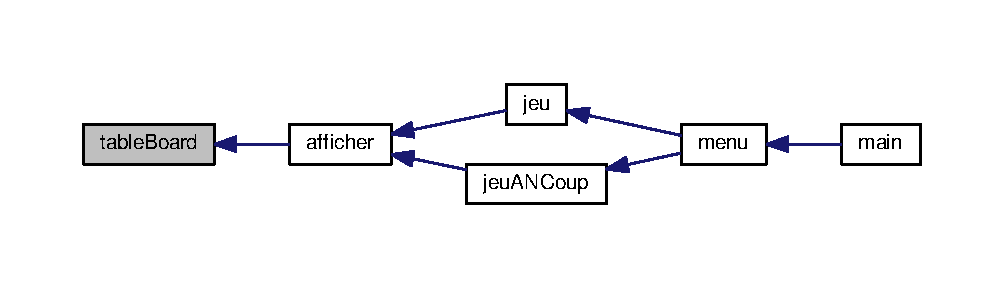
\includegraphics[width=350pt]{affichage_8c_a671ab408369ac69a9b4d3afc29c6fd21_icgraph}
\end{center}
\end{figure}

\hypertarget{header_8h}{}\section{Référence du fichier header.\+h}
\label{header_8h}\index{header.\+h@{header.\+h}}
{\ttfamily \#include $<$stdio.\+h$>$}\newline
{\ttfamily \#include $<$stdlib.\+h$>$}\newline
{\ttfamily \#include $<$time.\+h$>$}\newline
{\ttfamily \#include $<$assert.\+h$>$}\newline
Graphe des dépendances par inclusion de header.\+h\+:\nopagebreak
\begin{figure}[H]
\begin{center}
\leavevmode
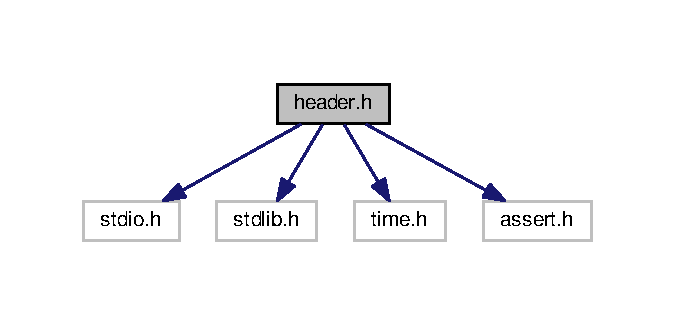
\includegraphics[width=324pt]{header_8h__incl}
\end{center}
\end{figure}
Ce graphe montre quels fichiers incluent directement ou indirectement ce fichier \+:\nopagebreak
\begin{figure}[H]
\begin{center}
\leavevmode
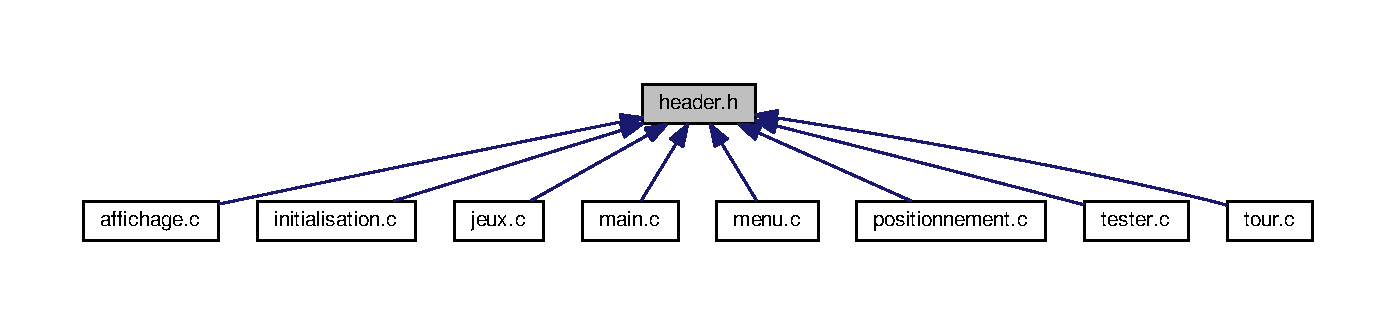
\includegraphics[width=350pt]{header_8h__dep__incl}
\end{center}
\end{figure}
\subsection*{Structures de données}
\begin{DoxyCompactItemize}
\item 
struct \mbox{\hyperlink{structbateau}{bateau}}
\begin{DoxyCompactList}\small\item\em Structure qui représente un bateau. \end{DoxyCompactList}\item 
struct \mbox{\hyperlink{structjoueur}{joueur}}
\begin{DoxyCompactList}\small\item\em Structure qui représente un joueur. \end{DoxyCompactList}\end{DoxyCompactItemize}
\subsection*{Macros}
\begin{DoxyCompactItemize}
\item 
\#define \mbox{\hyperlink{header_8h_aabcb2d6536b6c0ab41f99493c911489b}{couleur}}(param)~printf(\char`\"{}\textbackslash{}033\mbox{[}\%sm\char`\"{},param)
\begin{DoxyCompactList}\small\item\em Des macros qui nous permet d\textquotesingle{}afficher un texte en couleur passer en paramétre. \end{DoxyCompactList}\item 
\#define \mbox{\hyperlink{header_8h_a8d23feea868a983c8c2b661e1e16972f}{R\+ED}}~\char`\"{}31\char`\"{}
\item 
\#define \mbox{\hyperlink{header_8h_acfbc006ea433ad708fdee3e82996e721}{G\+R\+E\+EN}}~\char`\"{}32\char`\"{}
\item 
\#define \mbox{\hyperlink{header_8h_a79d10e672abb49ad63eeaa8aaef57c38}{B\+L\+UE}}~\char`\"{}34\char`\"{}
\item 
\#define \mbox{\hyperlink{header_8h_abf681265909adf3d3e8116c93c0ba179}{Y\+E\+L\+L\+OW}}~\char`\"{}33\char`\"{}
\item 
\#define \mbox{\hyperlink{header_8h_a87b537f5fa5c109d3c05c13d6b18f382}{W\+H\+I\+TE}}~\char`\"{}0\char`\"{}
\item 
\#define \mbox{\hyperlink{header_8h_adc3c2556e84bebbe78c8a87fc459a6f8}{T\+A\+I\+L\+L\+E\+\_\+\+P\+L\+A\+T\+E\+AU}}~15
\begin{DoxyCompactList}\small\item\em Des macros our supprimer l\textquotesingle{}écrans. \end{DoxyCompactList}\item 
\#define \mbox{\hyperlink{header_8h_a491086a202f32f357e418a99cde7156e}{N\+O\+M\+B\+R\+E\+\_\+\+C\+A\+S\+E\+\_\+\+B\+A\+T\+E\+AU}}~62
\item 
\#define \mbox{\hyperlink{header_8h_a56aaacd8cb8ffd138094887b2d3344f6}{N\+O\+M\+B\+R\+E\+\_\+\+B\+A\+T\+E\+AU}}~10
\end{DoxyCompactItemize}
\subsection*{Définitions de type}
\begin{DoxyCompactItemize}
\item 
typedef struct \mbox{\hyperlink{structbateau}{bateau}} \mbox{\hyperlink{header_8h_a1292ad8d8cbf040611a5322eb98e2564}{bateau}}
\item 
typedef struct \mbox{\hyperlink{structjoueur}{joueur}} \mbox{\hyperlink{header_8h_a1746f5078a33e091fd999b22274918c7}{joueur}}
\end{DoxyCompactItemize}
\subsection*{Fonctions}
\begin{DoxyCompactItemize}
\item 
void \mbox{\hyperlink{header_8h_a2a0e843767aeea4f433a28b9c54f573a}{menu}} ()
\begin{DoxyCompactList}\small\item\em Une fonction qui affiche le menu du jeu. \end{DoxyCompactList}\item 
void \mbox{\hyperlink{header_8h_a8e8142e641485c04318dde61025b95c1}{afficher}} (\mbox{\hyperlink{structjoueur}{joueur}} $\ast$, \mbox{\hyperlink{structjoueur}{joueur}} $\ast$, int)
\begin{DoxyCompactList}\small\item\em Une fonction qui affiche le plateau de jeu. \end{DoxyCompactList}\item 
void \mbox{\hyperlink{header_8h_aa7bd3bd80b4918740bf10a6b1fe3e57b}{print}} (\mbox{\hyperlink{structjoueur}{joueur}} $\ast$, int)
\begin{DoxyCompactList}\small\item\em Une fonction qui affiche différent messager de mise en forme dasn le jeu a l\textquotesingle{}aide d\textquotesingle{}un int donner comme argument. \end{DoxyCompactList}\item 
void \mbox{\hyperlink{header_8h_ad3e31aecff504dec8a8efee4b732c96c}{jeu}} (\mbox{\hyperlink{structjoueur}{joueur}} $\ast$, \mbox{\hyperlink{structjoueur}{joueur}} $\ast$)
\begin{DoxyCompactList}\small\item\em Une fonction qui déroule le jeu. \end{DoxyCompactList}\item 
void \mbox{\hyperlink{header_8h_abe8c11f21b141fd8d7826bebb3f1c46b}{jeu\+A\+N\+Coup}} (\mbox{\hyperlink{structjoueur}{joueur}} $\ast$, \mbox{\hyperlink{structjoueur}{joueur}} $\ast$, int)
\begin{DoxyCompactList}\small\item\em une fonction qui déroule jeu avancer de N coupe simuler \end{DoxyCompactList}\item 
void \mbox{\hyperlink{header_8h_a4bcd2f1cd82e9edd813bde29e9c12568}{table\+Board}} (\mbox{\hyperlink{structjoueur}{joueur}} $\ast$)
\begin{DoxyCompactList}\small\item\em Une fonction qui affiche le resultat du joueur actuelle à chaque tour. \end{DoxyCompactList}\item 
\mbox{\hyperlink{structjoueur}{joueur}} $\ast$ \mbox{\hyperlink{header_8h_aa69260c04e3640b56e402f842f5b7448}{initialisation}} (\mbox{\hyperlink{structjoueur}{joueur}} $\ast$, char $\ast$, int)
\begin{DoxyCompactList}\small\item\em Une fonction qui fait l\textquotesingle{}initialisation de chaque joueur au début du jeu. \end{DoxyCompactList}\item 
\mbox{\hyperlink{structjoueur}{joueur}} $\ast$ \mbox{\hyperlink{header_8h_a92c11248eb6a0ae0b0316938f3f07351}{positionement\+Des\+Bateaux}} (\mbox{\hyperlink{structjoueur}{joueur}} $\ast$)
\begin{DoxyCompactList}\small\item\em Une fonction qui posision les bateau de la bonne façon à chaque debut de jeu apres l\textquotesingle{}initialisation. \end{DoxyCompactList}\item 
\mbox{\hyperlink{structjoueur}{joueur}} $\ast$ \mbox{\hyperlink{header_8h_a92241da559f8c98b3ec5a99f4d151658}{tour}} (\mbox{\hyperlink{structjoueur}{joueur}} $\ast$, \mbox{\hyperlink{structjoueur}{joueur}} $\ast$)
\begin{DoxyCompactList}\small\item\em Une fonction qui déroule le tour d\textquotesingle{}un jour. \end{DoxyCompactList}\item 
int \mbox{\hyperlink{header_8h_a3106323267d0c2e16a73616d1666831a}{game\+Over}} (\mbox{\hyperlink{structjoueur}{joueur}} $\ast$)
\begin{DoxyCompactList}\small\item\em Une fonction qui vérifier la fin du jeu. \end{DoxyCompactList}\item 
void \mbox{\hyperlink{header_8h_adba405b6c8341bbae8459669db1aa775}{compar}} (int ligne, int colonne, \mbox{\hyperlink{structjoueur}{joueur}} $\ast$player, int choix, char $\ast$$\ast$\mbox{\hyperlink{header_8h_aabcb2d6536b6c0ab41f99493c911489b}{couleur}})
\begin{DoxyCompactList}\small\item\em Une fonction qui récupere une couleur selon des conditions. \end{DoxyCompactList}\end{DoxyCompactItemize}


\subsection{Description détaillée}
\begin{DoxyAuthor}{Auteur}
B.\+Habib, A.\+Sofiane, I.\+Tinhinane, I.\+Chafia 
\end{DoxyAuthor}
\begin{DoxyVersion}{Version}
1.\+0 
\end{DoxyVersion}
\begin{DoxyDate}{Date}
07 Avril 2018
\end{DoxyDate}
définition de la fonction tour 

\subsection{Documentation des macros}
\mbox{\Hypertarget{header_8h_a79d10e672abb49ad63eeaa8aaef57c38}\label{header_8h_a79d10e672abb49ad63eeaa8aaef57c38}} 
\index{header.\+h@{header.\+h}!B\+L\+UE@{B\+L\+UE}}
\index{B\+L\+UE@{B\+L\+UE}!header.\+h@{header.\+h}}
\subsubsection{\texorpdfstring{B\+L\+UE}{BLUE}}
{\footnotesize\ttfamily \#define B\+L\+UE~\char`\"{}34\char`\"{}}



Définition à la ligne 10 du fichier header.\+h.

\mbox{\Hypertarget{header_8h_aabcb2d6536b6c0ab41f99493c911489b}\label{header_8h_aabcb2d6536b6c0ab41f99493c911489b}} 
\index{header.\+h@{header.\+h}!couleur@{couleur}}
\index{couleur@{couleur}!header.\+h@{header.\+h}}
\subsubsection{\texorpdfstring{couleur}{couleur}}
{\footnotesize\ttfamily \#define couleur(\begin{DoxyParamCaption}\item[{}]{param }\end{DoxyParamCaption})~printf(\char`\"{}\textbackslash{}033\mbox{[}\%sm\char`\"{},param)}



Des macros qui nous permet d\textquotesingle{}afficher un texte en couleur passer en paramétre. 



Définition à la ligne 7 du fichier header.\+h.



Référencé par afficher(), compar(), print(), et table\+Board().

\mbox{\Hypertarget{header_8h_acfbc006ea433ad708fdee3e82996e721}\label{header_8h_acfbc006ea433ad708fdee3e82996e721}} 
\index{header.\+h@{header.\+h}!G\+R\+E\+EN@{G\+R\+E\+EN}}
\index{G\+R\+E\+EN@{G\+R\+E\+EN}!header.\+h@{header.\+h}}
\subsubsection{\texorpdfstring{G\+R\+E\+EN}{GREEN}}
{\footnotesize\ttfamily \#define G\+R\+E\+EN~\char`\"{}32\char`\"{}}



Définition à la ligne 9 du fichier header.\+h.



Référencé par main(), et menu().

\mbox{\Hypertarget{header_8h_a56aaacd8cb8ffd138094887b2d3344f6}\label{header_8h_a56aaacd8cb8ffd138094887b2d3344f6}} 
\index{header.\+h@{header.\+h}!N\+O\+M\+B\+R\+E\+\_\+\+B\+A\+T\+E\+AU@{N\+O\+M\+B\+R\+E\+\_\+\+B\+A\+T\+E\+AU}}
\index{N\+O\+M\+B\+R\+E\+\_\+\+B\+A\+T\+E\+AU@{N\+O\+M\+B\+R\+E\+\_\+\+B\+A\+T\+E\+AU}!header.\+h@{header.\+h}}
\subsubsection{\texorpdfstring{N\+O\+M\+B\+R\+E\+\_\+\+B\+A\+T\+E\+AU}{NOMBRE\_BATEAU}}
{\footnotesize\ttfamily \#define N\+O\+M\+B\+R\+E\+\_\+\+B\+A\+T\+E\+AU~10}



Définition à la ligne 22 du fichier header.\+h.



Référencé par compar(), initialisation(), positionement\+Des\+Bateaux(), table\+Board(), et tour().

\mbox{\Hypertarget{header_8h_a491086a202f32f357e418a99cde7156e}\label{header_8h_a491086a202f32f357e418a99cde7156e}} 
\index{header.\+h@{header.\+h}!N\+O\+M\+B\+R\+E\+\_\+\+C\+A\+S\+E\+\_\+\+B\+A\+T\+E\+AU@{N\+O\+M\+B\+R\+E\+\_\+\+C\+A\+S\+E\+\_\+\+B\+A\+T\+E\+AU}}
\index{N\+O\+M\+B\+R\+E\+\_\+\+C\+A\+S\+E\+\_\+\+B\+A\+T\+E\+AU@{N\+O\+M\+B\+R\+E\+\_\+\+C\+A\+S\+E\+\_\+\+B\+A\+T\+E\+AU}!header.\+h@{header.\+h}}
\subsubsection{\texorpdfstring{N\+O\+M\+B\+R\+E\+\_\+\+C\+A\+S\+E\+\_\+\+B\+A\+T\+E\+AU}{NOMBRE\_CASE\_BATEAU}}
{\footnotesize\ttfamily \#define N\+O\+M\+B\+R\+E\+\_\+\+C\+A\+S\+E\+\_\+\+B\+A\+T\+E\+AU~62}



Définition à la ligne 21 du fichier header.\+h.



Référencé par game\+Over().

\mbox{\Hypertarget{header_8h_a8d23feea868a983c8c2b661e1e16972f}\label{header_8h_a8d23feea868a983c8c2b661e1e16972f}} 
\index{header.\+h@{header.\+h}!R\+ED@{R\+ED}}
\index{R\+ED@{R\+ED}!header.\+h@{header.\+h}}
\subsubsection{\texorpdfstring{R\+ED}{RED}}
{\footnotesize\ttfamily \#define R\+ED~\char`\"{}31\char`\"{}}



Définition à la ligne 8 du fichier header.\+h.



Référencé par afficher(), et print().

\mbox{\Hypertarget{header_8h_adc3c2556e84bebbe78c8a87fc459a6f8}\label{header_8h_adc3c2556e84bebbe78c8a87fc459a6f8}} 
\index{header.\+h@{header.\+h}!T\+A\+I\+L\+L\+E\+\_\+\+P\+L\+A\+T\+E\+AU@{T\+A\+I\+L\+L\+E\+\_\+\+P\+L\+A\+T\+E\+AU}}
\index{T\+A\+I\+L\+L\+E\+\_\+\+P\+L\+A\+T\+E\+AU@{T\+A\+I\+L\+L\+E\+\_\+\+P\+L\+A\+T\+E\+AU}!header.\+h@{header.\+h}}
\subsubsection{\texorpdfstring{T\+A\+I\+L\+L\+E\+\_\+\+P\+L\+A\+T\+E\+AU}{TAILLE\_PLATEAU}}
{\footnotesize\ttfamily \#define T\+A\+I\+L\+L\+E\+\_\+\+P\+L\+A\+T\+E\+AU~15}



Des macros our supprimer l\textquotesingle{}écrans. 



Définition à la ligne 20 du fichier header.\+h.



Référencé par afficher(), initialisation(), positionement\+Des\+Bateaux(), et tour().

\mbox{\Hypertarget{header_8h_a87b537f5fa5c109d3c05c13d6b18f382}\label{header_8h_a87b537f5fa5c109d3c05c13d6b18f382}} 
\index{header.\+h@{header.\+h}!W\+H\+I\+TE@{W\+H\+I\+TE}}
\index{W\+H\+I\+TE@{W\+H\+I\+TE}!header.\+h@{header.\+h}}
\subsubsection{\texorpdfstring{W\+H\+I\+TE}{WHITE}}
{\footnotesize\ttfamily \#define W\+H\+I\+TE~\char`\"{}0\char`\"{}}



Définition à la ligne 12 du fichier header.\+h.



Référencé par afficher(), print(), et table\+Board().

\mbox{\Hypertarget{header_8h_abf681265909adf3d3e8116c93c0ba179}\label{header_8h_abf681265909adf3d3e8116c93c0ba179}} 
\index{header.\+h@{header.\+h}!Y\+E\+L\+L\+OW@{Y\+E\+L\+L\+OW}}
\index{Y\+E\+L\+L\+OW@{Y\+E\+L\+L\+OW}!header.\+h@{header.\+h}}
\subsubsection{\texorpdfstring{Y\+E\+L\+L\+OW}{YELLOW}}
{\footnotesize\ttfamily \#define Y\+E\+L\+L\+OW~\char`\"{}33\char`\"{}}



Définition à la ligne 11 du fichier header.\+h.



Référencé par main(), et menu().



\subsection{Documentation des définitions de type}
\mbox{\Hypertarget{header_8h_a1292ad8d8cbf040611a5322eb98e2564}\label{header_8h_a1292ad8d8cbf040611a5322eb98e2564}} 
\index{header.\+h@{header.\+h}!bateau@{bateau}}
\index{bateau@{bateau}!header.\+h@{header.\+h}}
\subsubsection{\texorpdfstring{bateau}{bateau}}
{\footnotesize\ttfamily typedef struct \mbox{\hyperlink{structbateau}{bateau}} \mbox{\hyperlink{structbateau}{bateau}}}



Définition à la ligne 37 du fichier header.\+h.

\mbox{\Hypertarget{header_8h_a1746f5078a33e091fd999b22274918c7}\label{header_8h_a1746f5078a33e091fd999b22274918c7}} 
\index{header.\+h@{header.\+h}!joueur@{joueur}}
\index{joueur@{joueur}!header.\+h@{header.\+h}}
\subsubsection{\texorpdfstring{joueur}{joueur}}
{\footnotesize\ttfamily typedef struct \mbox{\hyperlink{structjoueur}{joueur}} \mbox{\hyperlink{structjoueur}{joueur}}}



Définition à la ligne 52 du fichier header.\+h.



\subsection{Documentation des fonctions}
\mbox{\Hypertarget{header_8h_a8e8142e641485c04318dde61025b95c1}\label{header_8h_a8e8142e641485c04318dde61025b95c1}} 
\index{header.\+h@{header.\+h}!afficher@{afficher}}
\index{afficher@{afficher}!header.\+h@{header.\+h}}
\subsubsection{\texorpdfstring{afficher()}{afficher()}}
{\footnotesize\ttfamily void afficher (\begin{DoxyParamCaption}\item[{\mbox{\hyperlink{structjoueur}{joueur}} $\ast$}]{joueur1,  }\item[{\mbox{\hyperlink{structjoueur}{joueur}} $\ast$}]{joueur2,  }\item[{int}]{cacher }\end{DoxyParamCaption})}



Une fonction qui affiche le plateau de jeu. 

Cette fonction permet d\textquotesingle{}afficher tous le contenu du plateau les deux grilles des deux joueur une grille cacher du joueur adversaire et l\textquotesingle{}autre afficher normale celle du joueur actuelle. 
\begin{DoxyParams}{Paramètres}
{\em joueur$\ast$} & joueur1 \+: le joueur adversaire. \\
\hline
{\em joueur$\ast$} & joueur2 \+: le joueur actuelle. \\
\hline
{\em int} & cacher \+: une variable qui nous dit a ce que en fait un affichage cacher ou pas. \\
\hline
\end{DoxyParams}


Définition à la ligne 10 du fichier affichage.\+c.



Références joueur\+::color, compar(), couleur, joueur\+::nom, joueur\+::plateau, R\+ED, table\+Board(), T\+A\+I\+L\+L\+E\+\_\+\+P\+L\+A\+T\+E\+AU, et W\+H\+I\+TE.



Référencé par jeu(), et jeu\+A\+N\+Coup().


\begin{DoxyCode}
10                                                            \{
11     \textcolor{keywordtype}{int} ligne, colonne, i;
12     \textcolor{keywordtype}{char}* \mbox{\hyperlink{header_8h_aabcb2d6536b6c0ab41f99493c911489b}{couleur}};
13     \mbox{\hyperlink{affichage_8c_a671ab408369ac69a9b4d3afc29c6fd21}{tableBoard}}(joueur2); \textcolor{comment}{// lLa fonction qui affiche des informations sur le resultat du jeu pour
       chaque joueur }
14     \mbox{\hyperlink{header_8h_aabcb2d6536b6c0ab41f99493c911489b}{couleur}}(\textcolor{stringliteral}{"47"});\mbox{\hyperlink{header_8h_aabcb2d6536b6c0ab41f99493c911489b}{couleur}}(\mbox{\hyperlink{header_8h_a8d23feea868a983c8c2b661e1e16972f}{RED}});printf(\textcolor{stringliteral}{"\(\backslash\)t\(\backslash\)t  Plateau du joueur \%s  "},joueur1->
      \mbox{\hyperlink{structjoueur_a5228c842828b2639253cb7db01e6f72d}{nom}});\mbox{\hyperlink{header_8h_aabcb2d6536b6c0ab41f99493c911489b}{couleur}}(\mbox{\hyperlink{header_8h_a87b537f5fa5c109d3c05c13d6b18f382}{WHITE}});
15     \mbox{\hyperlink{header_8h_aabcb2d6536b6c0ab41f99493c911489b}{couleur}}(\textcolor{stringliteral}{"47"});\mbox{\hyperlink{header_8h_aabcb2d6536b6c0ab41f99493c911489b}{couleur}}(\mbox{\hyperlink{header_8h_a8d23feea868a983c8c2b661e1e16972f}{RED}});printf(\textcolor{stringliteral}{"\(\backslash\)t\(\backslash\)t\(\backslash\)t\(\backslash\)t\(\backslash\)t\(\backslash\)t\(\backslash\)t  Mon Plateau  \%s \(\backslash\)n"},joueur2->
      \mbox{\hyperlink{structjoueur_a5228c842828b2639253cb7db01e6f72d}{nom}});\mbox{\hyperlink{header_8h_aabcb2d6536b6c0ab41f99493c911489b}{couleur}}(\mbox{\hyperlink{header_8h_a87b537f5fa5c109d3c05c13d6b18f382}{WHITE}});
16     \textcolor{comment}{// Afficher les numeros de colonne pour la grille de l'adversaire  (player 1)}
17     \textcolor{keywordflow}{for}(colonne = 1 ; colonne <= \mbox{\hyperlink{header_8h_adc3c2556e84bebbe78c8a87fc459a6f8}{TAILLE\_PLATEAU}} ; ++colonne)
18         \textcolor{keywordflow}{if}(colonne < 10)
19             printf(\textcolor{stringliteral}{"  \%d "},colonne);
20         \textcolor{keywordflow}{else}
21             printf(\textcolor{stringliteral}{" \%d "},colonne);
22     printf(\textcolor{stringliteral}{"      "});
23     \textcolor{comment}{// Afficher les numeros de colonne pour la grille de jouer actuelle (player 2)}
24     \textcolor{keywordflow}{for}(colonne = 1 ; colonne <= \mbox{\hyperlink{header_8h_adc3c2556e84bebbe78c8a87fc459a6f8}{TAILLE\_PLATEAU}} ; ++colonne)
25         \textcolor{keywordflow}{if}(colonne < 10)
26             printf(\textcolor{stringliteral}{"  \%d "},colonne);
27         \textcolor{keywordflow}{else}
28             printf(\textcolor{stringliteral}{" \%d "},colonne);
29     printf(\textcolor{stringliteral}{"\(\backslash\)n"});
30 
31     \textcolor{keywordflow}{for}(ligne = 0 ; ligne < \mbox{\hyperlink{header_8h_adc3c2556e84bebbe78c8a87fc459a6f8}{TAILLE\_PLATEAU}} ; ++ligne)\{
32         printf(\textcolor{stringliteral}{"-"});
33         \textcolor{keywordflow}{for}(i = 0 ; i < \mbox{\hyperlink{header_8h_adc3c2556e84bebbe78c8a87fc459a6f8}{TAILLE\_PLATEAU}}; i++)  
34             printf(\textcolor{stringliteral}{"----"});
35         printf(\textcolor{stringliteral}{"     "});
36         printf(\textcolor{stringliteral}{"-"});
37         \textcolor{keywordflow}{for}(i = 0 ; i < \mbox{\hyperlink{header_8h_adc3c2556e84bebbe78c8a87fc459a6f8}{TAILLE\_PLATEAU}}; i++)  
38             printf(\textcolor{stringliteral}{"----"});
39         printf(\textcolor{stringliteral}{"\(\backslash\)n"});
40         \textcolor{comment}{// Afficher la grille de l'adversaire (joueur1) en cachent les bateaux non toucher }
41         \textcolor{keywordflow}{for}(colonne = 0 ; colonne < \mbox{\hyperlink{header_8h_adc3c2556e84bebbe78c8a87fc459a6f8}{TAILLE\_PLATEAU}} ; ++colonne)
42                 \textcolor{keywordflow}{if}(joueur1->\mbox{\hyperlink{structjoueur_a0de66c3578a57ff8e0ed1bf3d91c8e82}{plateau}}[ligne][colonne] == \textcolor{charliteral}{'\#'} \&\& cacher == 1)
43                     printf(\textcolor{stringliteral}{"|   "});
44                 \textcolor{keywordflow}{else} \textcolor{keywordflow}{if}(joueur1->\mbox{\hyperlink{structjoueur_a0de66c3578a57ff8e0ed1bf3d91c8e82}{plateau}}[ligne][colonne] == \textcolor{charliteral}{'X'})\{
45                     printf(\textcolor{stringliteral}{"| "});
46                     \mbox{\hyperlink{header_8h_aabcb2d6536b6c0ab41f99493c911489b}{couleur}} = \mbox{\hyperlink{header_8h_a8d23feea868a983c8c2b661e1e16972f}{RED}};
47                     \mbox{\hyperlink{affichage_8c_adba405b6c8341bbae8459669db1aa775}{compar}}(ligne, colonne, joueur1, 1, \&\mbox{\hyperlink{header_8h_aabcb2d6536b6c0ab41f99493c911489b}{couleur}});
48                     \mbox{\hyperlink{header_8h_aabcb2d6536b6c0ab41f99493c911489b}{couleur}}(\mbox{\hyperlink{header_8h_aabcb2d6536b6c0ab41f99493c911489b}{couleur}});
49                     printf(\textcolor{stringliteral}{"\%c "},joueur1->\mbox{\hyperlink{structjoueur_a0de66c3578a57ff8e0ed1bf3d91c8e82}{plateau}}[ligne][colonne]);
50                     \mbox{\hyperlink{header_8h_aabcb2d6536b6c0ab41f99493c911489b}{couleur}}(\mbox{\hyperlink{header_8h_a87b537f5fa5c109d3c05c13d6b18f382}{WHITE}});
51                 \}\textcolor{keywordflow}{else}\{
52                     printf(\textcolor{stringliteral}{"| "});
53                     \mbox{\hyperlink{header_8h_aabcb2d6536b6c0ab41f99493c911489b}{couleur}}(joueur1->\mbox{\hyperlink{structjoueur_a1064ba94d4d2719446f3c609135ba362}{color}});
54                     printf(\textcolor{stringliteral}{"\%c "},joueur1->\mbox{\hyperlink{structjoueur_a0de66c3578a57ff8e0ed1bf3d91c8e82}{plateau}}[ligne][colonne]);
55                     \mbox{\hyperlink{header_8h_aabcb2d6536b6c0ab41f99493c911489b}{couleur}}(\mbox{\hyperlink{header_8h_a87b537f5fa5c109d3c05c13d6b18f382}{WHITE}});
56                 \}
57         
58         \textcolor{keywordflow}{if}(ligne + 1 < 10)
59             printf(\textcolor{stringliteral}{"|  \%d  "}, ligne + 1);
60         \textcolor{keywordflow}{else}
61             printf(\textcolor{stringliteral}{"|  \%d "}, ligne + 1);
62         \textcolor{comment}{// Afficher la grille du joueur acctuelle (joueur2)  }
63         \textcolor{keywordflow}{for}(colonne = 0 ; colonne < \mbox{\hyperlink{header_8h_adc3c2556e84bebbe78c8a87fc459a6f8}{TAILLE\_PLATEAU}} ; ++colonne)
64                 \textcolor{keywordflow}{if}(joueur2->\mbox{\hyperlink{structjoueur_a0de66c3578a57ff8e0ed1bf3d91c8e82}{plateau}}[ligne][colonne] == \textcolor{charliteral}{'O'})
65                     printf(\textcolor{stringliteral}{"|   "});
66                 \textcolor{keywordflow}{else} \textcolor{keywordflow}{if}(joueur2->\mbox{\hyperlink{structjoueur_a0de66c3578a57ff8e0ed1bf3d91c8e82}{plateau}}[ligne][colonne] == \textcolor{charliteral}{'X'})\{
67                     \mbox{\hyperlink{header_8h_aabcb2d6536b6c0ab41f99493c911489b}{couleur}} = \mbox{\hyperlink{header_8h_a8d23feea868a983c8c2b661e1e16972f}{RED}};
68                     \mbox{\hyperlink{affichage_8c_adba405b6c8341bbae8459669db1aa775}{compar}}(ligne, colonne, joueur2, 1, \&\mbox{\hyperlink{header_8h_aabcb2d6536b6c0ab41f99493c911489b}{couleur}});
69                     printf(\textcolor{stringliteral}{"| "});
70                     \mbox{\hyperlink{header_8h_aabcb2d6536b6c0ab41f99493c911489b}{couleur}}(\mbox{\hyperlink{header_8h_aabcb2d6536b6c0ab41f99493c911489b}{couleur}});
71                     printf(\textcolor{stringliteral}{"\%c "},joueur2->\mbox{\hyperlink{structjoueur_a0de66c3578a57ff8e0ed1bf3d91c8e82}{plateau}}[ligne][colonne]);
72                     \mbox{\hyperlink{header_8h_aabcb2d6536b6c0ab41f99493c911489b}{couleur}}(\mbox{\hyperlink{header_8h_a87b537f5fa5c109d3c05c13d6b18f382}{WHITE}});
73                 \}\textcolor{keywordflow}{else}\{
74                     \mbox{\hyperlink{header_8h_aabcb2d6536b6c0ab41f99493c911489b}{couleur}} = joueur2->\mbox{\hyperlink{structjoueur_a1064ba94d4d2719446f3c609135ba362}{color}};
75                     \mbox{\hyperlink{affichage_8c_adba405b6c8341bbae8459669db1aa775}{compar}}(ligne, colonne, joueur2, 0, \&\mbox{\hyperlink{header_8h_aabcb2d6536b6c0ab41f99493c911489b}{couleur}});
76                     printf(\textcolor{stringliteral}{"| "});
77                     \mbox{\hyperlink{header_8h_aabcb2d6536b6c0ab41f99493c911489b}{couleur}}(\mbox{\hyperlink{header_8h_aabcb2d6536b6c0ab41f99493c911489b}{couleur}});
78                     printf(\textcolor{stringliteral}{"\%c "},joueur2->\mbox{\hyperlink{structjoueur_a0de66c3578a57ff8e0ed1bf3d91c8e82}{plateau}}[ligne][colonne]);
79                     \mbox{\hyperlink{header_8h_aabcb2d6536b6c0ab41f99493c911489b}{couleur}}(\mbox{\hyperlink{header_8h_a87b537f5fa5c109d3c05c13d6b18f382}{WHITE}});
80                 \}
81         printf(\textcolor{stringliteral}{"|\(\backslash\)n"});
82     \}
83  
84     printf(\textcolor{stringliteral}{"-"});
85     \textcolor{keywordflow}{for}(i = 0 ; i < \mbox{\hyperlink{header_8h_adc3c2556e84bebbe78c8a87fc459a6f8}{TAILLE\_PLATEAU}}; i++)  
86         printf(\textcolor{stringliteral}{"----"});
87     printf(\textcolor{stringliteral}{"     "});
88     printf(\textcolor{stringliteral}{"-"});
89     \textcolor{keywordflow}{for}(i = 0 ; i < \mbox{\hyperlink{header_8h_adc3c2556e84bebbe78c8a87fc459a6f8}{TAILLE\_PLATEAU}}; i++)  
90         printf(\textcolor{stringliteral}{"----"});
91     printf(\textcolor{stringliteral}{"\(\backslash\)n"});
92 \}
\end{DoxyCode}
Voici le graphe d\textquotesingle{}appel pour cette fonction \+:\nopagebreak
\begin{figure}[H]
\begin{center}
\leavevmode
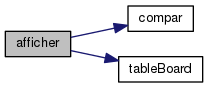
\includegraphics[width=228pt]{header_8h_a8e8142e641485c04318dde61025b95c1_cgraph}
\end{center}
\end{figure}
Voici le graphe des appelants de cette fonction \+:\nopagebreak
\begin{figure}[H]
\begin{center}
\leavevmode
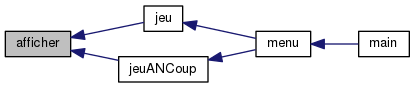
\includegraphics[width=350pt]{header_8h_a8e8142e641485c04318dde61025b95c1_icgraph}
\end{center}
\end{figure}
\mbox{\Hypertarget{header_8h_adba405b6c8341bbae8459669db1aa775}\label{header_8h_adba405b6c8341bbae8459669db1aa775}} 
\index{header.\+h@{header.\+h}!compar@{compar}}
\index{compar@{compar}!header.\+h@{header.\+h}}
\subsubsection{\texorpdfstring{compar()}{compar()}}
{\footnotesize\ttfamily void compar (\begin{DoxyParamCaption}\item[{int}]{ligne,  }\item[{int}]{colonne,  }\item[{\mbox{\hyperlink{structjoueur}{joueur}} $\ast$}]{player,  }\item[{int}]{choix,  }\item[{char $\ast$$\ast$}]{couleur }\end{DoxyParamCaption})}



Une fonction qui récupere une couleur selon des conditions. 

Cette fonction permet de récuperer soit la couleur real du bateau c\textquotesingle{}est choix==0, soit une autre couleur c\textquotesingle{}est tous le bateau est toucher 
\begin{DoxyParams}{Paramètres}
{\em int} & ligne \+: la ligne d\textquotesingle{}une case à tester. \\
\hline
{\em int} & colonne\+: la colonne d\textquotesingle{}une case à tester. \\
\hline
{\em joueur$\ast$} & player \+: le joueur actuelle. \\
\hline
{\em int} & choix \+: une variable qui nos sert à faire deux teste différent dans une fonction. \\
\hline
{\em char$\ast$$\ast$} & couleur \+: une pointeur sur la variable couleur. \\
\hline
\end{DoxyParams}


Définition à la ligne 152 du fichier affichage.\+c.



Références joueur\+::bat, bateau\+::color, couleur, bateau\+::nbr\+\_\+case\+\_\+colonne, bateau\+::nbr\+\_\+case\+\_\+ligne, bateau\+::nbr\+\_\+case\+\_\+total, bateau\+::nbr\+\_\+case\+\_\+toucher, N\+O\+M\+B\+R\+E\+\_\+\+B\+A\+T\+E\+AU, bateau\+::position\+\_\+colonne, et bateau\+::position\+\_\+ligne.



Référencé par afficher().


\begin{DoxyCode}
152                                                                               \{
153     \textcolor{keywordtype}{int} test, i;
154     \textcolor{keywordflow}{for} (i = 0; i < \mbox{\hyperlink{header_8h_a56aaacd8cb8ffd138094887b2d3344f6}{NOMBRE\_BATEAU}}; ++i)\{
155         test = ((colonne >= player->\mbox{\hyperlink{structjoueur_a3b21aa14ce27f69126dc9a649b363146}{bat}}[i].\mbox{\hyperlink{structbateau_aac775edde7cde57176e580c29f6e8eca}{position\_colonne}}) \&\& (colonne < player->
      \mbox{\hyperlink{structjoueur_a3b21aa14ce27f69126dc9a649b363146}{bat}}[i].position\_colonne + player->\mbox{\hyperlink{structjoueur_a3b21aa14ce27f69126dc9a649b363146}{bat}}[i].\mbox{\hyperlink{structbateau_a1a56dd379e7c5cfc5714fd204947a0a8}{nbr\_case\_colonne}})) 
156                 \&\&((ligne >= player->\mbox{\hyperlink{structjoueur_a3b21aa14ce27f69126dc9a649b363146}{bat}}[i].\mbox{\hyperlink{structbateau_a5dcd33e534b9b1b8b0414325bc5c09b1}{position\_ligne}}) \&\& (ligne < player->
      \mbox{\hyperlink{structjoueur_a3b21aa14ce27f69126dc9a649b363146}{bat}}[i].\mbox{\hyperlink{structbateau_a5dcd33e534b9b1b8b0414325bc5c09b1}{position\_ligne}} + player->\mbox{\hyperlink{structjoueur_a3b21aa14ce27f69126dc9a649b363146}{bat}}[i].\mbox{\hyperlink{structbateau_a5f7637b2932717e5589e1a368dd1b47b}{nbr\_case\_ligne}}));
157 
158         \textcolor{keywordflow}{if}(test \&\& (player->\mbox{\hyperlink{structjoueur_a3b21aa14ce27f69126dc9a649b363146}{bat}}[i].\mbox{\hyperlink{structbateau_aff445dc58a52069759f1e4bfd13c0313}{nbr\_case\_total}} == player->
      \mbox{\hyperlink{structjoueur_a3b21aa14ce27f69126dc9a649b363146}{bat}}[i].\mbox{\hyperlink{structbateau_a62ae80832c521a9984c520fde88dadfd}{nbr\_case\_toucher}}) \&\& (choix == 1))\{       
159             *\mbox{\hyperlink{header_8h_aabcb2d6536b6c0ab41f99493c911489b}{couleur}} = \textcolor{stringliteral}{"40"};
160             \textcolor{keywordflow}{break};
161         \}
162         \textcolor{keywordflow}{if}(test \&\& (choix == 0))\{
163             *\mbox{\hyperlink{header_8h_aabcb2d6536b6c0ab41f99493c911489b}{couleur}} = player->\mbox{\hyperlink{structjoueur_a3b21aa14ce27f69126dc9a649b363146}{bat}}[i].\mbox{\hyperlink{structbateau_a41910d4781ab6f3256d23f62b98c49a1}{color}};
164             \textcolor{keywordflow}{break};
165         \}
166     \}
167 \}
\end{DoxyCode}
Voici le graphe des appelants de cette fonction \+:\nopagebreak
\begin{figure}[H]
\begin{center}
\leavevmode
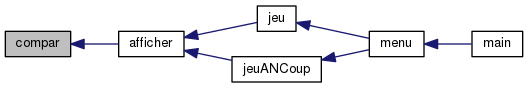
\includegraphics[width=350pt]{header_8h_adba405b6c8341bbae8459669db1aa775_icgraph}
\end{center}
\end{figure}
\mbox{\Hypertarget{header_8h_a3106323267d0c2e16a73616d1666831a}\label{header_8h_a3106323267d0c2e16a73616d1666831a}} 
\index{header.\+h@{header.\+h}!game\+Over@{game\+Over}}
\index{game\+Over@{game\+Over}!header.\+h@{header.\+h}}
\subsubsection{\texorpdfstring{game\+Over()}{gameOver()}}
{\footnotesize\ttfamily int game\+Over (\begin{DoxyParamCaption}\item[{\mbox{\hyperlink{structjoueur}{joueur}} $\ast$}]{player }\end{DoxyParamCaption})}



Une fonction qui vérifier la fin du jeu. 

Cette fonction permet de savoir la fin du jeu en testent l\textquotesingle{}égaliter entre le nombre de tir reussit et le nombre de case total pour l\textquotesingle{}ensemble des bateaux ~\newline

\begin{DoxyParams}{Paramètres}
{\em joueur$\ast$} & player \+: le joueur concerner. \\
\hline
\end{DoxyParams}


Définition à la ligne 8 du fichier jeux.\+c.



Références joueur\+::nbr\+\_\+tir\+\_\+reussit, N\+O\+M\+B\+R\+E\+\_\+\+C\+A\+S\+E\+\_\+\+B\+A\+T\+E\+AU, et print().



Référencé par jeu(), jeu\+A\+N\+Coup(), et main().


\begin{DoxyCode}
8                             \{
9   \textcolor{keywordflow}{if}(player->\mbox{\hyperlink{structjoueur_a19510a02b4ff3f6336da487b50806d71}{nbr\_tir\_reussit}} == \mbox{\hyperlink{header_8h_a491086a202f32f357e418a99cde7156e}{NOMBRE\_CASE\_BATEAU}})\{
10     \mbox{\hyperlink{affichage_8c_a34b6e28e00a180632a300b9608ad6acd}{print}}(player, 2);
11     \textcolor{keywordflow}{return} 1;
12   \}
13   \textcolor{keywordflow}{else} 
14     \textcolor{keywordflow}{return} 0; 
15 \}
\end{DoxyCode}
Voici le graphe d\textquotesingle{}appel pour cette fonction \+:\nopagebreak
\begin{figure}[H]
\begin{center}
\leavevmode
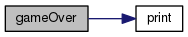
\includegraphics[width=213pt]{header_8h_a3106323267d0c2e16a73616d1666831a_cgraph}
\end{center}
\end{figure}
Voici le graphe des appelants de cette fonction \+:\nopagebreak
\begin{figure}[H]
\begin{center}
\leavevmode
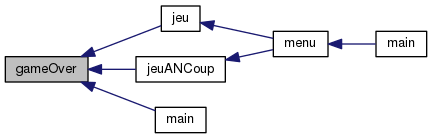
\includegraphics[width=350pt]{header_8h_a3106323267d0c2e16a73616d1666831a_icgraph}
\end{center}
\end{figure}
\mbox{\Hypertarget{header_8h_aa69260c04e3640b56e402f842f5b7448}\label{header_8h_aa69260c04e3640b56e402f842f5b7448}} 
\index{header.\+h@{header.\+h}!initialisation@{initialisation}}
\index{initialisation@{initialisation}!header.\+h@{header.\+h}}
\subsubsection{\texorpdfstring{initialisation()}{initialisation()}}
{\footnotesize\ttfamily \mbox{\hyperlink{structjoueur}{joueur}}$\ast$ initialisation (\begin{DoxyParamCaption}\item[{\mbox{\hyperlink{structjoueur}{joueur}} $\ast$}]{player,  }\item[{char $\ast$}]{color,  }\item[{int}]{ia }\end{DoxyParamCaption})}



Une fonction qui fait l\textquotesingle{}initialisation de chaque joueur au début du jeu. 

Cette fonction permet d\textquotesingle{}intialiser les champ du joueur passer en argument. 
\begin{DoxyParams}{Paramètres}
{\em joueur$\ast$} & player \+: le joueur. \\
\hline
{\em char$\ast$} & color \+: la couleur par défaut du joueur. \\
\hline
{\em int} & ia \+: une valeur qui indique la nature du joueur humaine ou ia. \\
\hline
\end{DoxyParams}
\begin{DoxyReturn}{Renvoie}
le joueur. 
\end{DoxyReturn}


Définition à la ligne 10 du fichier initialisation.\+c.



Références joueur\+::color, joueur\+::ia, joueur\+::nbr\+\_\+bateau\+\_\+couler, joueur\+::nbr\+\_\+bateau\+\_\+restant, joueur\+::nbr\+\_\+tir\+\_\+manquer, joueur\+::nbr\+\_\+tir\+\_\+reussit, joueur\+::nom, N\+O\+M\+B\+R\+E\+\_\+\+B\+A\+T\+E\+AU, joueur\+::plateau, positionement\+Des\+Bateaux(), et T\+A\+I\+L\+L\+E\+\_\+\+P\+L\+A\+T\+E\+AU.



Référencé par main(), et menu().


\begin{DoxyCode}
10                                                            \{
11     \textcolor{keywordtype}{int} ligne, colonne;
12     player = malloc(\textcolor{keyword}{sizeof} (*player));
13     printf(\textcolor{stringliteral}{"Donner Le  Nom Du Joueur:"});
14     player->\mbox{\hyperlink{structjoueur_a5228c842828b2639253cb7db01e6f72d}{nom}} = malloc(10 * \textcolor{keyword}{sizeof}(\textcolor{keywordtype}{char}));
15     scanf(\textcolor{stringliteral}{"\%s"},player->\mbox{\hyperlink{structjoueur_a5228c842828b2639253cb7db01e6f72d}{nom}});
16     
17     \textcolor{keywordflow}{for}(ligne = 0 ; ligne < \mbox{\hyperlink{header_8h_adc3c2556e84bebbe78c8a87fc459a6f8}{TAILLE\_PLATEAU}} ; ++ligne)
18         \textcolor{keywordflow}{for}(colonne = 0 ; colonne < \mbox{\hyperlink{header_8h_adc3c2556e84bebbe78c8a87fc459a6f8}{TAILLE\_PLATEAU}} ; ++colonne)
19             player->\mbox{\hyperlink{structjoueur_a0de66c3578a57ff8e0ed1bf3d91c8e82}{plateau}}[ligne][colonne] = \textcolor{charliteral}{' '};
20 
21     player->\mbox{\hyperlink{structjoueur_a307e3b4b4c1b78e753c599bc1f6a47c3}{ia}} = \mbox{\hyperlink{structjoueur_a307e3b4b4c1b78e753c599bc1f6a47c3}{ia}};
22     player->\mbox{\hyperlink{structjoueur_ab0c0fa544d83148d4daed41c84954e55}{nbr\_bateau\_couler}} = 0;
23     player->\mbox{\hyperlink{structjoueur_a4f902c486f8d66cb85cf3b07abd0bd12}{nbr\_bateau\_restant}} = \mbox{\hyperlink{header_8h_a56aaacd8cb8ffd138094887b2d3344f6}{NOMBRE\_BATEAU}};
24     player->\mbox{\hyperlink{structjoueur_a19510a02b4ff3f6336da487b50806d71}{nbr\_tir\_reussit}} = 0;
25     player->\mbox{\hyperlink{structjoueur_aaba095a23d03a15d363924e77caa3c1e}{nbr\_tir\_manquer}} = 0;
26     player->\mbox{\hyperlink{structjoueur_a1064ba94d4d2719446f3c609135ba362}{color}} = \mbox{\hyperlink{structjoueur_a1064ba94d4d2719446f3c609135ba362}{color}};
27     
28     player = \mbox{\hyperlink{header_8h_a92c11248eb6a0ae0b0316938f3f07351}{positionementDesBateaux}}(player);
29     \textcolor{keywordflow}{return} player;
30 \}
\end{DoxyCode}
Voici le graphe d\textquotesingle{}appel pour cette fonction \+:\nopagebreak
\begin{figure}[H]
\begin{center}
\leavevmode
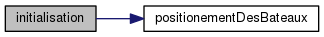
\includegraphics[width=315pt]{header_8h_aa69260c04e3640b56e402f842f5b7448_cgraph}
\end{center}
\end{figure}
Voici le graphe des appelants de cette fonction \+:\nopagebreak
\begin{figure}[H]
\begin{center}
\leavevmode
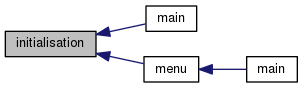
\includegraphics[width=299pt]{header_8h_aa69260c04e3640b56e402f842f5b7448_icgraph}
\end{center}
\end{figure}
\mbox{\Hypertarget{header_8h_ad3e31aecff504dec8a8efee4b732c96c}\label{header_8h_ad3e31aecff504dec8a8efee4b732c96c}} 
\index{header.\+h@{header.\+h}!jeu@{jeu}}
\index{jeu@{jeu}!header.\+h@{header.\+h}}
\subsubsection{\texorpdfstring{jeu()}{jeu()}}
{\footnotesize\ttfamily void jeu (\begin{DoxyParamCaption}\item[{\mbox{\hyperlink{structjoueur}{joueur}} $\ast$}]{player1,  }\item[{\mbox{\hyperlink{structjoueur}{joueur}} $\ast$}]{player2 }\end{DoxyParamCaption})}



Une fonction qui déroule le jeu. 

Cette fonction permet de jouer à une partie du jeu. 
\begin{DoxyParams}{Paramètres}
{\em joueur$\ast$} & player1 \+: le joueur 1. \\
\hline
{\em joueur$\ast$} & player2 \+: le joueur 2. \\
\hline
\end{DoxyParams}


Définition à la ligne 22 du fichier jeux.\+c.



Références afficher(), game\+Over(), joueur\+::ia, print(), et tour().



Référencé par menu().


\begin{DoxyCode}
22                                          \{
23   \mbox{\hyperlink{structjoueur}{joueur}}* joueurActualle;
24   \textcolor{keywordtype}{int} i = 0;
25     
26   joueurActualle = player1;
27   \mbox{\hyperlink{affichage_8c_a34b6e28e00a180632a300b9608ad6acd}{print}}(joueurActualle,3);
28   \textcolor{keywordflow}{while}(!\mbox{\hyperlink{jeux_8c_a3610cb607e2029a8583ce054be882fbc}{gameOver}}(joueurActualle))\{
29   \textcolor{comment}{// Le joueur 1 jeu son tour}
30     joueurActualle = player1;
31     \textcolor{keywordflow}{if}(player1->\mbox{\hyperlink{structjoueur_a307e3b4b4c1b78e753c599bc1f6a47c3}{ia}} == player2->\mbox{\hyperlink{structjoueur_a307e3b4b4c1b78e753c599bc1f6a47c3}{ia}})\{
32       \mbox{\hyperlink{affichage_8c_a34b6e28e00a180632a300b9608ad6acd}{print}}(joueurActualle, 1);
33       \mbox{\hyperlink{affichage_8c_a8004c5a076f6d53e90583b921ac810cb}{afficher}}(player2, player1,1);
34     \}
35     \textcolor{comment}{// Le joueur 1 choisit une case du plateau du joueur 2 }
36     player2 = \mbox{\hyperlink{header_8h_a92241da559f8c98b3ec5a99f4d151658}{tour}}(player1, player2);
37     \textcolor{keywordflow}{if}(player1->\mbox{\hyperlink{structjoueur_a307e3b4b4c1b78e753c599bc1f6a47c3}{ia}} == player2->\mbox{\hyperlink{structjoueur_a307e3b4b4c1b78e753c599bc1f6a47c3}{ia}}) \mbox{\hyperlink{affichage_8c_a34b6e28e00a180632a300b9608ad6acd}{print}}(joueurActualle, 0);
38     \textcolor{comment}{//On teste c'est le joueur 1  à gagner}
39     \textcolor{keywordflow}{if}(!\mbox{\hyperlink{jeux_8c_a3610cb607e2029a8583ce054be882fbc}{gameOver}}(joueurActualle))\{
40     \textcolor{comment}{// Le joueur 2 jeu son tour}
41       joueurActualle = player2;
42       \mbox{\hyperlink{affichage_8c_a34b6e28e00a180632a300b9608ad6acd}{print}}(joueurActualle, 1);  
43       \mbox{\hyperlink{affichage_8c_a8004c5a076f6d53e90583b921ac810cb}{afficher}}(player1, player2,1);
44       \textcolor{comment}{// Le joueur 2 choisit une case du plateau du joueur 1}
45       player1 = \mbox{\hyperlink{header_8h_a92241da559f8c98b3ec5a99f4d151658}{tour}}(player2, player1);      
46       \mbox{\hyperlink{affichage_8c_a34b6e28e00a180632a300b9608ad6acd}{print}}(joueurActualle, 0);
47     \}\textcolor{keywordflow}{else}\{
48       \textcolor{keywordflow}{break};
49     \}
50     i++;
51   \}
52   printf(\textcolor{stringliteral}{"Le nombre de tour joue = \%d\(\backslash\)n"},i);
53 \}
\end{DoxyCode}
Voici le graphe d\textquotesingle{}appel pour cette fonction \+:\nopagebreak
\begin{figure}[H]
\begin{center}
\leavevmode
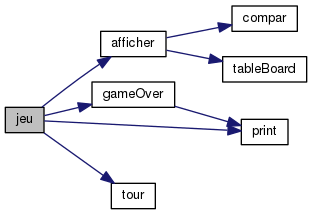
\includegraphics[width=306pt]{header_8h_ad3e31aecff504dec8a8efee4b732c96c_cgraph}
\end{center}
\end{figure}
Voici le graphe des appelants de cette fonction \+:\nopagebreak
\begin{figure}[H]
\begin{center}
\leavevmode
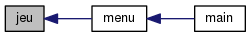
\includegraphics[width=260pt]{header_8h_ad3e31aecff504dec8a8efee4b732c96c_icgraph}
\end{center}
\end{figure}
\mbox{\Hypertarget{header_8h_abe8c11f21b141fd8d7826bebb3f1c46b}\label{header_8h_abe8c11f21b141fd8d7826bebb3f1c46b}} 
\index{header.\+h@{header.\+h}!jeu\+A\+N\+Coup@{jeu\+A\+N\+Coup}}
\index{jeu\+A\+N\+Coup@{jeu\+A\+N\+Coup}!header.\+h@{header.\+h}}
\subsubsection{\texorpdfstring{jeu\+A\+N\+Coup()}{jeuANCoup()}}
{\footnotesize\ttfamily void jeu\+A\+N\+Coup (\begin{DoxyParamCaption}\item[{\mbox{\hyperlink{structjoueur}{joueur}} $\ast$}]{player1,  }\item[{\mbox{\hyperlink{structjoueur}{joueur}} $\ast$}]{player2,  }\item[{int}]{n }\end{DoxyParamCaption})}



une fonction qui déroule jeu avancer de N coupe simuler 

Cette fonction permet d\textquotesingle{}avancer la parti à un coup. 
\begin{DoxyParams}{Paramètres}
{\em joueur$\ast$} & player1 \+: le joueur 1. \\
\hline
{\em joueur$\ast$} & player2 \+: le joueur 2. \\
\hline
{\em int} & n \+: le nombre de tour que on veut avancé le jeu. \\
\hline
\end{DoxyParams}


Définition à la ligne 61 du fichier jeux.\+c.



Références afficher(), game\+Over(), joueur\+::ia, print(), et tour().



Référencé par menu().


\begin{DoxyCode}
61                                                      \{
62   \mbox{\hyperlink{structjoueur}{joueur}}* joueurActualle = player1;
63   \textcolor{keywordtype}{int} i = 0, ia1 = player1->\mbox{\hyperlink{structjoueur_a307e3b4b4c1b78e753c599bc1f6a47c3}{ia}}, ia2 = player2->\mbox{\hyperlink{structjoueur_a307e3b4b4c1b78e753c599bc1f6a47c3}{ia}};
64 
65   \mbox{\hyperlink{affichage_8c_a34b6e28e00a180632a300b9608ad6acd}{print}}(joueurActualle,3);
66   player1->\mbox{\hyperlink{structjoueur_a307e3b4b4c1b78e753c599bc1f6a47c3}{ia}} = 1;
67   player2->\mbox{\hyperlink{structjoueur_a307e3b4b4c1b78e753c599bc1f6a47c3}{ia}} = 1;
68   \textcolor{keywordflow}{while}(!\mbox{\hyperlink{jeux_8c_a3610cb607e2029a8583ce054be882fbc}{gameOver}}(joueurActualle) \&\& (i < n))\{
69     joueurActualle = player1;
70     player2 = \mbox{\hyperlink{header_8h_a92241da559f8c98b3ec5a99f4d151658}{tour}}(player1, player2);
71     \textcolor{keywordflow}{if}(!\mbox{\hyperlink{jeux_8c_a3610cb607e2029a8583ce054be882fbc}{gameOver}}(joueurActualle))\{
72       joueurActualle = player2;
73       player1 = \mbox{\hyperlink{header_8h_a92241da559f8c98b3ec5a99f4d151658}{tour}}(player2, player1);
74     \}
75     i++;
76   \}
77   player1->\mbox{\hyperlink{structjoueur_a307e3b4b4c1b78e753c599bc1f6a47c3}{ia}} = ia1;
78   player2->\mbox{\hyperlink{structjoueur_a307e3b4b4c1b78e753c599bc1f6a47c3}{ia}} = ia2;
79   \textcolor{keywordflow}{while}(!\mbox{\hyperlink{jeux_8c_a3610cb607e2029a8583ce054be882fbc}{gameOver}}(joueurActualle))\{
80     joueurActualle = player1;
81     \mbox{\hyperlink{affichage_8c_a34b6e28e00a180632a300b9608ad6acd}{print}}(joueurActualle, 1);
82     \mbox{\hyperlink{affichage_8c_a8004c5a076f6d53e90583b921ac810cb}{afficher}}(player2, player1, 1);
83     player2 = \mbox{\hyperlink{header_8h_a92241da559f8c98b3ec5a99f4d151658}{tour}}(player1, player2);
84     \mbox{\hyperlink{affichage_8c_a34b6e28e00a180632a300b9608ad6acd}{print}}(player2, 0);
85 
86     \textcolor{keywordflow}{if}(!\mbox{\hyperlink{jeux_8c_a3610cb607e2029a8583ce054be882fbc}{gameOver}}(joueurActualle))\{
87       joueurActualle = player2;
88       \mbox{\hyperlink{affichage_8c_a34b6e28e00a180632a300b9608ad6acd}{print}}(joueurActualle, 1);
89       \mbox{\hyperlink{affichage_8c_a8004c5a076f6d53e90583b921ac810cb}{afficher}}(player1, player2, 1);
90       player1 = \mbox{\hyperlink{header_8h_a92241da559f8c98b3ec5a99f4d151658}{tour}}(player2, player1);
91       \mbox{\hyperlink{affichage_8c_a34b6e28e00a180632a300b9608ad6acd}{print}}(player2, 0);
92     \}\textcolor{keywordflow}{else} 
93       \textcolor{keywordflow}{break};
94     i++;
95   \}
96   printf(\textcolor{stringliteral}{"Le nombre de tour joue = \%d\(\backslash\)n"},i);
97 \}
\end{DoxyCode}
Voici le graphe d\textquotesingle{}appel pour cette fonction \+:\nopagebreak
\begin{figure}[H]
\begin{center}
\leavevmode
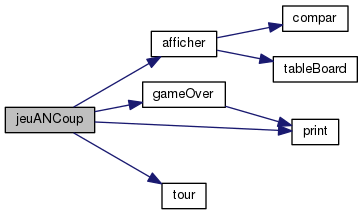
\includegraphics[width=344pt]{header_8h_abe8c11f21b141fd8d7826bebb3f1c46b_cgraph}
\end{center}
\end{figure}
Voici le graphe des appelants de cette fonction \+:\nopagebreak
\begin{figure}[H]
\begin{center}
\leavevmode
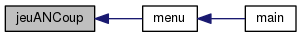
\includegraphics[width=298pt]{header_8h_abe8c11f21b141fd8d7826bebb3f1c46b_icgraph}
\end{center}
\end{figure}
\mbox{\Hypertarget{header_8h_a2a0e843767aeea4f433a28b9c54f573a}\label{header_8h_a2a0e843767aeea4f433a28b9c54f573a}} 
\index{header.\+h@{header.\+h}!menu@{menu}}
\index{menu@{menu}!header.\+h@{header.\+h}}
\subsubsection{\texorpdfstring{menu()}{menu()}}
{\footnotesize\ttfamily void menu (\begin{DoxyParamCaption}{ }\end{DoxyParamCaption})}



Une fonction qui affiche le menu du jeu. 

Cette fonction permet d\textquotesingle{}afficher le menu principale du jeu. 

Définition à la ligne 6 du fichier menu.\+c.



Références G\+R\+E\+EN, initialisation(), jeu(), jeu\+A\+N\+Coup(), et Y\+E\+L\+L\+OW.



Référencé par main().


\begin{DoxyCode}
6            \{
7 srand(time(NULL));
8 \mbox{\hyperlink{structjoueur}{joueur}}* joueur1;
9 \mbox{\hyperlink{structjoueur}{joueur}}* joueur2;
10 \textcolor{keywordtype}{int} choix,n;
11 \textcolor{keywordflow}{do}\{
12   CLEAR\_SCREEN;
13   printf(\textcolor{stringliteral}{"\(\backslash\)t\(\backslash\)t\(\backslash\)033[42mBATAILLE NAVALE\(\backslash\)033[0m\(\backslash\)n"});
14   printf(\textcolor{stringliteral}{"\(\backslash\)033[35m----------------------------------------------------------\(\backslash\)n"});
15   printf(\textcolor{stringliteral}{"\(\backslash\)033[35m|\(\backslash\)033[33m1-\(\backslash\)033[32mPartie :\(\backslash\)033[34m Humain vs Humain\(\backslash\)033[37m                           \(\backslash\)0
      33[35m|\(\backslash\)n"});
16   printf(\textcolor{stringliteral}{"\(\backslash\)033[35m|\(\backslash\)033[33m2-\(\backslash\)033[32mPartie :\(\backslash\)033[34m Ordi vs Ordi\(\backslash\)033[37m                         \(\backslash\)0
      33[35m|\(\backslash\)n"});
17   printf(\textcolor{stringliteral}{"\(\backslash\)033[35m|\(\backslash\)033[33m3-\(\backslash\)033[32mPartie :\(\backslash\)033[34m Humain vs Ordi\(\backslash\)033[37m                         \(\backslash\)0
      33[35m|\(\backslash\)n"});
18   printf(\textcolor{stringliteral}{"\(\backslash\)033[35m|\(\backslash\)033[33m4-\(\backslash\)033[32mPartie :\(\backslash\)033[34m Humain vs Humain Partier Avancer de n coupe\(\backslash\)033[37m  
      \(\backslash\)033[35m|\(\backslash\)n"});
19   printf(\textcolor{stringliteral}{"\(\backslash\)033[35m|\(\backslash\)033[33m5-\(\backslash\)033[31mQuitter                                               \(\backslash\)033[35m|\(\backslash\)n"});
20   printf(\textcolor{stringliteral}{"----------------------------------------------------------\(\backslash\)n"});
21   printf(\textcolor{stringliteral}{"\(\backslash\)033[37mChoisir Dans Le Menu :"});
22 
23   \textcolor{keywordflow}{do} \{
24     scanf(\textcolor{stringliteral}{"\%d"},\&choix);
25   \}\textcolor{keywordflow}{while}((choix != 1)\&\&(choix != 2)\&\&(choix != 3)\&\&(choix != 4)\&\&(choix != 5));
26   CLEAR\_SCREEN;
27   \textcolor{keywordflow}{switch} (choix) \{
28     \textcolor{keywordflow}{case} 1:\{
29       joueur1 = \mbox{\hyperlink{header_8h_aa69260c04e3640b56e402f842f5b7448}{initialisation}}(joueur1,\mbox{\hyperlink{header_8h_acfbc006ea433ad708fdee3e82996e721}{GREEN}},0);
30       joueur2 = \mbox{\hyperlink{header_8h_aa69260c04e3640b56e402f842f5b7448}{initialisation}}(joueur2,\mbox{\hyperlink{header_8h_abf681265909adf3d3e8116c93c0ba179}{YELLOW}},0);
31       \mbox{\hyperlink{header_8h_ad3e31aecff504dec8a8efee4b732c96c}{jeu}}(joueur1,joueur2);
32     \}
33     \textcolor{keywordflow}{break};
34     \textcolor{keywordflow}{case} 2:\{
35       joueur1 = \mbox{\hyperlink{header_8h_aa69260c04e3640b56e402f842f5b7448}{initialisation}}(joueur1,\mbox{\hyperlink{header_8h_acfbc006ea433ad708fdee3e82996e721}{GREEN}},1);
36       joueur2 = \mbox{\hyperlink{header_8h_aa69260c04e3640b56e402f842f5b7448}{initialisation}}(joueur2,\mbox{\hyperlink{header_8h_abf681265909adf3d3e8116c93c0ba179}{YELLOW}},1);
37       \mbox{\hyperlink{header_8h_ad3e31aecff504dec8a8efee4b732c96c}{jeu}}(joueur1,joueur2);
38     \}
39     \textcolor{keywordflow}{break};
40     \textcolor{keywordflow}{case} 3:\{
41       joueur1 = \mbox{\hyperlink{header_8h_aa69260c04e3640b56e402f842f5b7448}{initialisation}}(joueur1,\mbox{\hyperlink{header_8h_acfbc006ea433ad708fdee3e82996e721}{GREEN}},0);
42       joueur2 = \mbox{\hyperlink{header_8h_aa69260c04e3640b56e402f842f5b7448}{initialisation}}(joueur2,\mbox{\hyperlink{header_8h_abf681265909adf3d3e8116c93c0ba179}{YELLOW}},1);
43       \mbox{\hyperlink{header_8h_ad3e31aecff504dec8a8efee4b732c96c}{jeu}}(joueur1,joueur2);
44     \}
45     \textcolor{keywordflow}{break};
46     \textcolor{keywordflow}{case} 4:\{
47       printf(\textcolor{stringliteral}{"Donner l'etape du jeu souhaité :"});
48       \textcolor{keywordflow}{do} \{
49         scanf(\textcolor{stringliteral}{"\%d"},\&n);
50       \}\textcolor{keywordflow}{while}(n < 0);
51       joueur1 = \mbox{\hyperlink{header_8h_aa69260c04e3640b56e402f842f5b7448}{initialisation}}(joueur1,\mbox{\hyperlink{header_8h_acfbc006ea433ad708fdee3e82996e721}{GREEN}},0);
52       joueur2 = \mbox{\hyperlink{header_8h_aa69260c04e3640b56e402f842f5b7448}{initialisation}}(joueur2,\mbox{\hyperlink{header_8h_abf681265909adf3d3e8116c93c0ba179}{YELLOW}},0);
53       \mbox{\hyperlink{header_8h_abe8c11f21b141fd8d7826bebb3f1c46b}{jeuANCoup}}(joueur1,joueur2,n);
54     \}
55     \textcolor{keywordflow}{break};
56     \textcolor{keywordflow}{case} 5:\{
57       printf(\textcolor{stringliteral}{"Au-revoir à La Prochaine fois ^-^  ^-^  ^-^ \(\backslash\)n"});
58       system(\textcolor{stringliteral}{"exit"});
59     \}
60     \textcolor{keywordflow}{break};
61   \}
62 \}\textcolor{keywordflow}{while}(choix!=5);
63 \}
\end{DoxyCode}
Voici le graphe d\textquotesingle{}appel pour cette fonction \+:\nopagebreak
\begin{figure}[H]
\begin{center}
\leavevmode
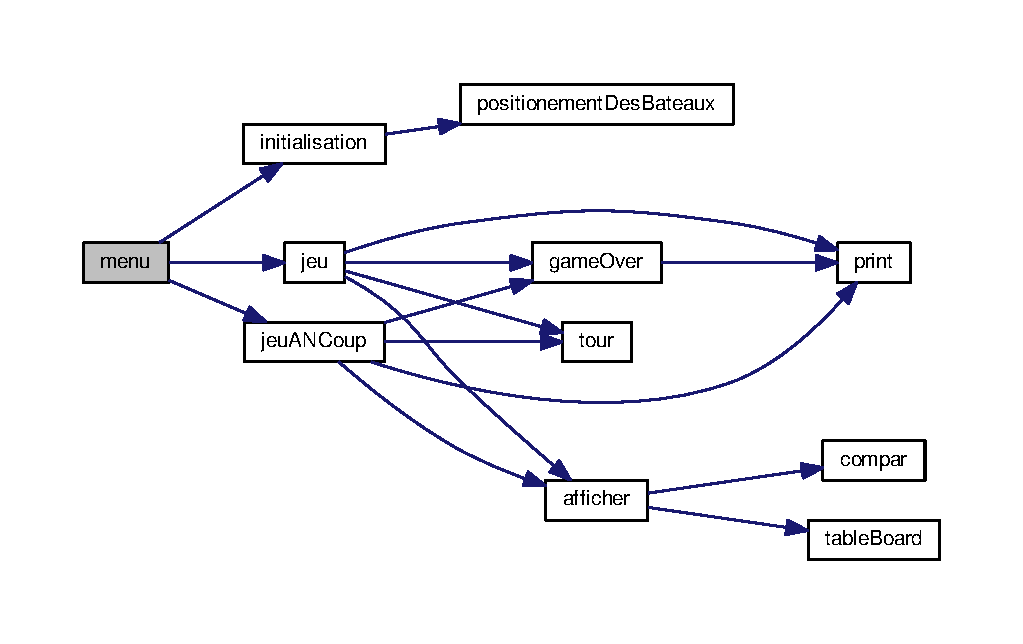
\includegraphics[width=350pt]{header_8h_a2a0e843767aeea4f433a28b9c54f573a_cgraph}
\end{center}
\end{figure}
Voici le graphe des appelants de cette fonction \+:\nopagebreak
\begin{figure}[H]
\begin{center}
\leavevmode
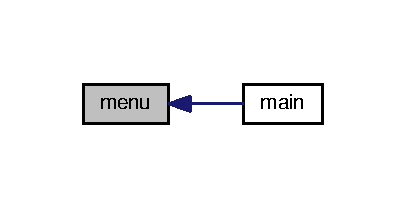
\includegraphics[width=195pt]{header_8h_a2a0e843767aeea4f433a28b9c54f573a_icgraph}
\end{center}
\end{figure}
\mbox{\Hypertarget{header_8h_a92c11248eb6a0ae0b0316938f3f07351}\label{header_8h_a92c11248eb6a0ae0b0316938f3f07351}} 
\index{header.\+h@{header.\+h}!positionement\+Des\+Bateaux@{positionement\+Des\+Bateaux}}
\index{positionement\+Des\+Bateaux@{positionement\+Des\+Bateaux}!header.\+h@{header.\+h}}
\subsubsection{\texorpdfstring{positionement\+Des\+Bateaux()}{positionementDesBateaux()}}
{\footnotesize\ttfamily \mbox{\hyperlink{structjoueur}{joueur}}$\ast$ positionement\+Des\+Bateaux (\begin{DoxyParamCaption}\item[{\mbox{\hyperlink{structjoueur}{joueur}} $\ast$}]{player }\end{DoxyParamCaption})}



Une fonction qui posision les bateau de la bonne façon à chaque debut de jeu apres l\textquotesingle{}initialisation. 

Cette fonction permet de positionner les bateaux. 
\begin{DoxyParams}{Paramètres}
{\em joueur$\ast$} & player \+: le joueur concerner. \\
\hline
\end{DoxyParams}
\begin{DoxyReturn}{Renvoie}
Le joueur. 
\end{DoxyReturn}


Définition à la ligne 8 du fichier positionnement.\+c.



Références joueur\+::bat, bateau\+::color, bateau\+::nbr\+\_\+case\+\_\+colonne, bateau\+::nbr\+\_\+case\+\_\+ligne, bateau\+::nbr\+\_\+case\+\_\+total, bateau\+::nbr\+\_\+case\+\_\+toucher, N\+O\+M\+B\+R\+E\+\_\+\+B\+A\+T\+E\+AU, bateau\+::normale, joueur\+::plateau, bateau\+::position\+\_\+colonne, bateau\+::position\+\_\+ligne, T\+A\+I\+L\+L\+E\+\_\+\+P\+L\+A\+T\+E\+AU, et bateau\+::type.



Référencé par initialisation().


\begin{DoxyCode}
8                                                \{
9     \textcolor{keywordtype}{int} nbrCase = 2, occuper, choix1, choix2;
10     \textcolor{keywordtype}{int} posc, posl;
11     \textcolor{comment}{// Les 4 Bateaux sous forme de  ligne}
12     \textcolor{keywordflow}{for}(\textcolor{keywordtype}{int} i = 0; i < 4;i++)\{
13         player->\mbox{\hyperlink{structjoueur_a3b21aa14ce27f69126dc9a649b363146}{bat}}[i].\mbox{\hyperlink{structbateau_a1a56dd379e7c5cfc5714fd204947a0a8}{nbr\_case\_colonne}} = nbrCase++;
14         player->\mbox{\hyperlink{structjoueur_a3b21aa14ce27f69126dc9a649b363146}{bat}}[i].\mbox{\hyperlink{structbateau_a5f7637b2932717e5589e1a368dd1b47b}{nbr\_case\_ligne}} = 1;
15     \}
16     \textcolor{comment}{// Les Couleur donner pour chaque bateaux}
17     player->\mbox{\hyperlink{structjoueur_a3b21aa14ce27f69126dc9a649b363146}{bat}}[0].\mbox{\hyperlink{structbateau_a41910d4781ab6f3256d23f62b98c49a1}{color}} = \textcolor{stringliteral}{"32"};player->\mbox{\hyperlink{structjoueur_a3b21aa14ce27f69126dc9a649b363146}{bat}}[1].\mbox{\hyperlink{structbateau_a41910d4781ab6f3256d23f62b98c49a1}{color}} = \textcolor{stringliteral}{"33"};player->
      \mbox{\hyperlink{structjoueur_a3b21aa14ce27f69126dc9a649b363146}{bat}}[2].\mbox{\hyperlink{structbateau_a41910d4781ab6f3256d23f62b98c49a1}{color}} = \textcolor{stringliteral}{"34"};player->\mbox{\hyperlink{structjoueur_a3b21aa14ce27f69126dc9a649b363146}{bat}}[3].\mbox{\hyperlink{structbateau_a41910d4781ab6f3256d23f62b98c49a1}{color}} = \textcolor{stringliteral}{"35"};
18     player->\mbox{\hyperlink{structjoueur_a3b21aa14ce27f69126dc9a649b363146}{bat}}[4].\mbox{\hyperlink{structbateau_a41910d4781ab6f3256d23f62b98c49a1}{color}} = \textcolor{stringliteral}{"36"};player->\mbox{\hyperlink{structjoueur_a3b21aa14ce27f69126dc9a649b363146}{bat}}[5].\mbox{\hyperlink{structbateau_a41910d4781ab6f3256d23f62b98c49a1}{color}} = \textcolor{stringliteral}{"37"};player->
      \mbox{\hyperlink{structjoueur_a3b21aa14ce27f69126dc9a649b363146}{bat}}[6].\mbox{\hyperlink{structbateau_a41910d4781ab6f3256d23f62b98c49a1}{color}} = \textcolor{stringliteral}{"38"};player->\mbox{\hyperlink{structjoueur_a3b21aa14ce27f69126dc9a649b363146}{bat}}[7].\mbox{\hyperlink{structbateau_a41910d4781ab6f3256d23f62b98c49a1}{color}} = \textcolor{stringliteral}{"36"};
19     player->\mbox{\hyperlink{structjoueur_a3b21aa14ce27f69126dc9a649b363146}{bat}}[8].\mbox{\hyperlink{structbateau_a41910d4781ab6f3256d23f62b98c49a1}{color}} = \textcolor{stringliteral}{"32"};player->\mbox{\hyperlink{structjoueur_a3b21aa14ce27f69126dc9a649b363146}{bat}}[9].\mbox{\hyperlink{structbateau_a41910d4781ab6f3256d23f62b98c49a1}{color}} = \textcolor{stringliteral}{"33"};
20     \textcolor{comment}{// Les bateaux sous forme de 4x4 et 4x2}
21     player->\mbox{\hyperlink{structjoueur_a3b21aa14ce27f69126dc9a649b363146}{bat}}[4].\mbox{\hyperlink{structbateau_a1a56dd379e7c5cfc5714fd204947a0a8}{nbr\_case\_colonne}} = player->\mbox{\hyperlink{structjoueur_a3b21aa14ce27f69126dc9a649b363146}{bat}}[4].
      \mbox{\hyperlink{structbateau_a5f7637b2932717e5589e1a368dd1b47b}{nbr\_case\_ligne}} = 2;
22     player->\mbox{\hyperlink{structjoueur_a3b21aa14ce27f69126dc9a649b363146}{bat}}[5].\mbox{\hyperlink{structbateau_a1a56dd379e7c5cfc5714fd204947a0a8}{nbr\_case\_colonne}} = 4;player->\mbox{\hyperlink{structjoueur_a3b21aa14ce27f69126dc9a649b363146}{bat}}[5].
      \mbox{\hyperlink{structbateau_a5f7637b2932717e5589e1a368dd1b47b}{nbr\_case\_ligne}} = 2;
23     player->\mbox{\hyperlink{structjoueur_a3b21aa14ce27f69126dc9a649b363146}{bat}}[6].\mbox{\hyperlink{structbateau_a1a56dd379e7c5cfc5714fd204947a0a8}{nbr\_case\_colonne}} = player->\mbox{\hyperlink{structjoueur_a3b21aa14ce27f69126dc9a649b363146}{bat}}[6].
      \mbox{\hyperlink{structbateau_a5f7637b2932717e5589e1a368dd1b47b}{nbr\_case\_ligne}} = 4;
24     \textcolor{comment}{// on fait la déffirence  entre les bateaux normale(bateaux ligne, 4x4 et 4x2) est anormale(bateaux L,
       H et T)  }
25     \textcolor{keywordflow}{for} (\textcolor{keywordtype}{int} i = 0; i <= 6; ++i)\{   
26         player->\mbox{\hyperlink{structjoueur_a3b21aa14ce27f69126dc9a649b363146}{bat}}[i].\mbox{\hyperlink{structbateau_ac4078d21fa180ff7d5c7e7fbf8a4a773}{type}} = 0;\textcolor{comment}{// pour faire la deffirence entre les forme des bateaux}
27         player->\mbox{\hyperlink{structjoueur_a3b21aa14ce27f69126dc9a649b363146}{bat}}[i].\mbox{\hyperlink{structbateau_a77fe0bf7801ff08bf9b17e6c6237692e}{normale}} = 0;
28         player->\mbox{\hyperlink{structjoueur_a3b21aa14ce27f69126dc9a649b363146}{bat}}[i].\mbox{\hyperlink{structbateau_aff445dc58a52069759f1e4bfd13c0313}{nbr\_case\_total}} = player->\mbox{\hyperlink{structjoueur_a3b21aa14ce27f69126dc9a649b363146}{bat}}[i].
      \mbox{\hyperlink{structbateau_a5f7637b2932717e5589e1a368dd1b47b}{nbr\_case\_ligne}} * player->\mbox{\hyperlink{structjoueur_a3b21aa14ce27f69126dc9a649b363146}{bat}}[i].\mbox{\hyperlink{structbateau_a1a56dd379e7c5cfc5714fd204947a0a8}{nbr\_case\_colonne}};\textcolor{comment}{// Nombre total de case
       pour chaque  bateau}
29     \}
30     \textcolor{comment}{// Les bateau sous forme de L, H et T}
31     player->\mbox{\hyperlink{structjoueur_a3b21aa14ce27f69126dc9a649b363146}{bat}}[7].\mbox{\hyperlink{structbateau_a1a56dd379e7c5cfc5714fd204947a0a8}{nbr\_case\_colonne}} = player->\mbox{\hyperlink{structjoueur_a3b21aa14ce27f69126dc9a649b363146}{bat}}[7].
      \mbox{\hyperlink{structbateau_a5f7637b2932717e5589e1a368dd1b47b}{nbr\_case\_ligne}} = 4; player->\mbox{\hyperlink{structjoueur_a3b21aa14ce27f69126dc9a649b363146}{bat}}[7].\mbox{\hyperlink{structbateau_a77fe0bf7801ff08bf9b17e6c6237692e}{normale}} = 1; player->
      \mbox{\hyperlink{structjoueur_a3b21aa14ce27f69126dc9a649b363146}{bat}}[7].\mbox{\hyperlink{structbateau_ac4078d21fa180ff7d5c7e7fbf8a4a773}{type}} = 1; player->\mbox{\hyperlink{structjoueur_a3b21aa14ce27f69126dc9a649b363146}{bat}}[7].\mbox{\hyperlink{structbateau_aff445dc58a52069759f1e4bfd13c0313}{nbr\_case\_total}} = 7;
32     player->\mbox{\hyperlink{structjoueur_a3b21aa14ce27f69126dc9a649b363146}{bat}}[8].\mbox{\hyperlink{structbateau_a1a56dd379e7c5cfc5714fd204947a0a8}{nbr\_case\_colonne}} = 3; player->\mbox{\hyperlink{structjoueur_a3b21aa14ce27f69126dc9a649b363146}{bat}}[8].
      \mbox{\hyperlink{structbateau_a5f7637b2932717e5589e1a368dd1b47b}{nbr\_case\_ligne}} = 4; player->\mbox{\hyperlink{structjoueur_a3b21aa14ce27f69126dc9a649b363146}{bat}}[8].\mbox{\hyperlink{structbateau_a77fe0bf7801ff08bf9b17e6c6237692e}{normale}} = 1; player->
      \mbox{\hyperlink{structjoueur_a3b21aa14ce27f69126dc9a649b363146}{bat}}[8].\mbox{\hyperlink{structbateau_ac4078d21fa180ff7d5c7e7fbf8a4a773}{type}} = 2; player->\mbox{\hyperlink{structjoueur_a3b21aa14ce27f69126dc9a649b363146}{bat}}[8].\mbox{\hyperlink{structbateau_aff445dc58a52069759f1e4bfd13c0313}{nbr\_case\_total}} = 6;
33     player->\mbox{\hyperlink{structjoueur_a3b21aa14ce27f69126dc9a649b363146}{bat}}[9].\mbox{\hyperlink{structbateau_a1a56dd379e7c5cfc5714fd204947a0a8}{nbr\_case\_colonne}} = player->\mbox{\hyperlink{structjoueur_a3b21aa14ce27f69126dc9a649b363146}{bat}}[9].
      \mbox{\hyperlink{structbateau_a5f7637b2932717e5589e1a368dd1b47b}{nbr\_case\_ligne}} = 3; player->\mbox{\hyperlink{structjoueur_a3b21aa14ce27f69126dc9a649b363146}{bat}}[9].\mbox{\hyperlink{structbateau_a77fe0bf7801ff08bf9b17e6c6237692e}{normale}} = 1; player->
      \mbox{\hyperlink{structjoueur_a3b21aa14ce27f69126dc9a649b363146}{bat}}[9].\mbox{\hyperlink{structbateau_ac4078d21fa180ff7d5c7e7fbf8a4a773}{type}} = 3; player->\mbox{\hyperlink{structjoueur_a3b21aa14ce27f69126dc9a649b363146}{bat}}[9].\mbox{\hyperlink{structbateau_aff445dc58a52069759f1e4bfd13c0313}{nbr\_case\_total}} = 7;
34     \textcolor{comment}{// Placement des Bateaux dans le plateau}
35     \textcolor{keywordflow}{for}(\textcolor{keywordtype}{int} i = 0 ; i < \mbox{\hyperlink{header_8h_a56aaacd8cb8ffd138094887b2d3344f6}{NOMBRE\_BATEAU}} ; i++)\{
36         player->\mbox{\hyperlink{structjoueur_a3b21aa14ce27f69126dc9a649b363146}{bat}}[i].\mbox{\hyperlink{structbateau_a62ae80832c521a9984c520fde88dadfd}{nbr\_case\_toucher}} = 0;\textcolor{comment}{// Au debut aucune case n'est toucher }
37         \textcolor{comment}{//chercher une bonne position pour chaque bateau}
38         \textcolor{keywordflow}{do}\{
39             occuper = 0;
40             posc = rand() \% (\mbox{\hyperlink{header_8h_adc3c2556e84bebbe78c8a87fc459a6f8}{TAILLE\_PLATEAU}} - player->\mbox{\hyperlink{structjoueur_a3b21aa14ce27f69126dc9a649b363146}{bat}}[i].
      \mbox{\hyperlink{structbateau_a1a56dd379e7c5cfc5714fd204947a0a8}{nbr\_case\_colonne}} + 1);\textcolor{comment}{// Colonne de positionement du bateau}
41             posl = rand() \% (\mbox{\hyperlink{header_8h_adc3c2556e84bebbe78c8a87fc459a6f8}{TAILLE\_PLATEAU}} - player->\mbox{\hyperlink{structjoueur_a3b21aa14ce27f69126dc9a649b363146}{bat}}[i].
      \mbox{\hyperlink{structbateau_a5f7637b2932717e5589e1a368dd1b47b}{nbr\_case\_ligne}} + 1); \textcolor{comment}{// Ligne de positionement du bateau}
42             \textcolor{comment}{//printf("posl = \%d   posc = \%d \(\backslash\)n",posl,posc);}
43             \textcolor{comment}{// Vérifié si il y n'a pas un autre bateau sur cette position}
44             \textcolor{keywordflow}{for}(\textcolor{keywordtype}{int} j = posl ; j < posl + player->\mbox{\hyperlink{structjoueur_a3b21aa14ce27f69126dc9a649b363146}{bat}}[i].\mbox{\hyperlink{structbateau_a5f7637b2932717e5589e1a368dd1b47b}{nbr\_case\_ligne}} ; j++)\{
45                 \textcolor{keywordflow}{for}(\textcolor{keywordtype}{int} k = posc ; k < posc + player->\mbox{\hyperlink{structjoueur_a3b21aa14ce27f69126dc9a649b363146}{bat}}[i].\mbox{\hyperlink{structbateau_a1a56dd379e7c5cfc5714fd204947a0a8}{nbr\_case\_colonne}} ; ++k)\{
46                     \textcolor{keywordflow}{if}(player->\mbox{\hyperlink{structjoueur_a0de66c3578a57ff8e0ed1bf3d91c8e82}{plateau}}[j][k] == \textcolor{charliteral}{'\#'})\{
47                         occuper = 1;
48                         \textcolor{keywordflow}{break};
49                     \}
50                 \}   
51                 \textcolor{keywordflow}{if}(occuper == 1)\textcolor{keywordflow}{break};
52             \}
53             \textcolor{keywordflow}{if}(player->\mbox{\hyperlink{structjoueur_a3b21aa14ce27f69126dc9a649b363146}{bat}}[i].\mbox{\hyperlink{structbateau_a77fe0bf7801ff08bf9b17e6c6237692e}{normale}})\{
54                 \textcolor{keywordflow}{for} (\textcolor{keywordtype}{int} j = 0; j < i; ++j)\{
55                     \textcolor{keywordflow}{if}(((posc >= player-> \mbox{\hyperlink{structjoueur_a3b21aa14ce27f69126dc9a649b363146}{bat}}[i].\mbox{\hyperlink{structbateau_aac775edde7cde57176e580c29f6e8eca}{position\_colonne}})
56                             \&\& (posc < player-> \mbox{\hyperlink{structjoueur_a3b21aa14ce27f69126dc9a649b363146}{bat}}[j].\mbox{\hyperlink{structbateau_aac775edde7cde57176e580c29f6e8eca}{position\_colonne}} + player-> 
      \mbox{\hyperlink{structjoueur_a3b21aa14ce27f69126dc9a649b363146}{bat}}[j].\mbox{\hyperlink{structbateau_a1a56dd379e7c5cfc5714fd204947a0a8}{nbr\_case\_colonne}})) \&\&
57                             ((posl >= player-> \mbox{\hyperlink{structjoueur_a3b21aa14ce27f69126dc9a649b363146}{bat}}[j].\mbox{\hyperlink{structbateau_a5dcd33e534b9b1b8b0414325bc5c09b1}{position\_ligne}})
58                             \&\& (posl < player-> \mbox{\hyperlink{structjoueur_a3b21aa14ce27f69126dc9a649b363146}{bat}}[j].position\_ligne + player-> 
      \mbox{\hyperlink{structjoueur_a3b21aa14ce27f69126dc9a649b363146}{bat}}[j].\mbox{\hyperlink{structbateau_a5f7637b2932717e5589e1a368dd1b47b}{nbr\_case\_ligne}})))\{
59                         occuper = 1;
60                         \textcolor{keywordflow}{break};
61                     \}
62                 \}
63             \}
64         \} \textcolor{keywordflow}{while} (occuper == 1);\textcolor{comment}{// repeter tanque il y déja un bateau sur cette position }
65         \textcolor{comment}{//Affecter la bonne position au bateau }
66         player->\mbox{\hyperlink{structjoueur_a3b21aa14ce27f69126dc9a649b363146}{bat}}[i].\mbox{\hyperlink{structbateau_a5dcd33e534b9b1b8b0414325bc5c09b1}{position\_ligne}} = posl; 
67         player->\mbox{\hyperlink{structjoueur_a3b21aa14ce27f69126dc9a649b363146}{bat}}[i].\mbox{\hyperlink{structbateau_aac775edde7cde57176e580c29f6e8eca}{position\_colonne}} = posc;
68         \textcolor{comment}{// Dessiner le bateau selon sa forme (ligne, 4x4, 4x2, L, H et T ...)}
69         \textcolor{keywordflow}{if}(player->\mbox{\hyperlink{structjoueur_a3b21aa14ce27f69126dc9a649b363146}{bat}}[i].\mbox{\hyperlink{structbateau_a77fe0bf7801ff08bf9b17e6c6237692e}{normale}} == 0)\{
70             \textcolor{keywordflow}{for}(\textcolor{keywordtype}{int} j = posl ; j < posl + player->\mbox{\hyperlink{structjoueur_a3b21aa14ce27f69126dc9a649b363146}{bat}}[i].\mbox{\hyperlink{structbateau_a5f7637b2932717e5589e1a368dd1b47b}{nbr\_case\_ligne}} ; j++)
71                 \textcolor{keywordflow}{for}(\textcolor{keywordtype}{int} k = posc ; k < posc + player->\mbox{\hyperlink{structjoueur_a3b21aa14ce27f69126dc9a649b363146}{bat}}[i].\mbox{\hyperlink{structbateau_a1a56dd379e7c5cfc5714fd204947a0a8}{nbr\_case\_colonne}} ; ++k)
72                     player->\mbox{\hyperlink{structjoueur_a0de66c3578a57ff8e0ed1bf3d91c8e82}{plateau}}[j][k] = \textcolor{charliteral}{'\#'};
73         \}\textcolor{keywordflow}{else}\{
74             \textcolor{keywordflow}{switch} (player->\mbox{\hyperlink{structjoueur_a3b21aa14ce27f69126dc9a649b363146}{bat}}[i].\mbox{\hyperlink{structbateau_ac4078d21fa180ff7d5c7e7fbf8a4a773}{type}})\{
75                 \textcolor{keywordflow}{case} 1 :\{\textcolor{comment}{// Bateau sous forme de L 4 cas}
76                     choix1 = rand()\%3 + 1;
77                     choix2 = rand()\%3 + 1;
78                     \textcolor{keywordflow}{if}(choix2 == 2 ) choix2 = posl + player->\mbox{\hyperlink{structjoueur_a3b21aa14ce27f69126dc9a649b363146}{bat}}[i].
      \mbox{\hyperlink{structbateau_a5f7637b2932717e5589e1a368dd1b47b}{nbr\_case\_ligne}} - 1 ;
79                     \textcolor{keywordflow}{else} choix2 = posl ;
80 
81                     \textcolor{keywordflow}{if}(choix1 == 2 ) choix1 = posc + player->\mbox{\hyperlink{structjoueur_a3b21aa14ce27f69126dc9a649b363146}{bat}}[i].
      \mbox{\hyperlink{structbateau_a1a56dd379e7c5cfc5714fd204947a0a8}{nbr\_case\_colonne}} - 1 ;
82                     \textcolor{keywordflow}{else} choix1 = posc ;
83                 \}
84                 \textcolor{keywordflow}{break};
85                 \textcolor{keywordflow}{case} 2 :\{\textcolor{comment}{// Bateau sous forme de T}
86                     choix1 = posc + player->\mbox{\hyperlink{structjoueur_a3b21aa14ce27f69126dc9a649b363146}{bat}}[i].\mbox{\hyperlink{structbateau_a1a56dd379e7c5cfc5714fd204947a0a8}{nbr\_case\_colonne}}/2;
87                     choix2 = posl;
88                 \}
89                 \textcolor{keywordflow}{break};
90                 \textcolor{keywordflow}{case} 3 :\{\textcolor{comment}{// Bateau sous forme de H}
91                     choix1 = posc + player->\mbox{\hyperlink{structjoueur_a3b21aa14ce27f69126dc9a649b363146}{bat}}[i].\mbox{\hyperlink{structbateau_a1a56dd379e7c5cfc5714fd204947a0a8}{nbr\_case\_colonne}} - 1;
92                     choix2 = posl + player->\mbox{\hyperlink{structjoueur_a3b21aa14ce27f69126dc9a649b363146}{bat}}[i].\mbox{\hyperlink{structbateau_a5f7637b2932717e5589e1a368dd1b47b}{nbr\_case\_ligne}} / 2;
93                 \}
94                 \textcolor{keywordflow}{break};
95             \}
96             \textcolor{comment}{// Placer les bateaux dans le plateau }
97             \textcolor{keywordflow}{for}(\textcolor{keywordtype}{int} j = posl ; j < posl + player->\mbox{\hyperlink{structjoueur_a3b21aa14ce27f69126dc9a649b363146}{bat}}[i].\mbox{\hyperlink{structbateau_a5f7637b2932717e5589e1a368dd1b47b}{nbr\_case\_ligne}} ; j++)
98                 player->\mbox{\hyperlink{structjoueur_a0de66c3578a57ff8e0ed1bf3d91c8e82}{plateau}}[j][choix1] = \textcolor{charliteral}{'\#'};
99 
100             \textcolor{keywordflow}{if}(player->\mbox{\hyperlink{structjoueur_a3b21aa14ce27f69126dc9a649b363146}{bat}}[i].\mbox{\hyperlink{structbateau_ac4078d21fa180ff7d5c7e7fbf8a4a773}{type}} == 3)\{
101                 \textcolor{keywordflow}{for}(\textcolor{keywordtype}{int} j = posl ; j < posl + player->\mbox{\hyperlink{structjoueur_a3b21aa14ce27f69126dc9a649b363146}{bat}}[i].\mbox{\hyperlink{structbateau_a5f7637b2932717e5589e1a368dd1b47b}{nbr\_case\_ligne}} ; j++)
102                 player->\mbox{\hyperlink{structjoueur_a0de66c3578a57ff8e0ed1bf3d91c8e82}{plateau}}[j][posc] = \textcolor{charliteral}{'\#'};
103             \}
104 
105             \textcolor{keywordflow}{for}(\textcolor{keywordtype}{int} k = posc ; k < posc + player->\mbox{\hyperlink{structjoueur_a3b21aa14ce27f69126dc9a649b363146}{bat}}[i].\mbox{\hyperlink{structbateau_a1a56dd379e7c5cfc5714fd204947a0a8}{nbr\_case\_colonne}} ; ++k) 
106                 player->\mbox{\hyperlink{structjoueur_a0de66c3578a57ff8e0ed1bf3d91c8e82}{plateau}}[choix2][k] = \textcolor{charliteral}{'\#'};
107         \}
108     \}
109 
110 \textcolor{keywordflow}{return} player;
111 \}
\end{DoxyCode}
Voici le graphe des appelants de cette fonction \+:\nopagebreak
\begin{figure}[H]
\begin{center}
\leavevmode
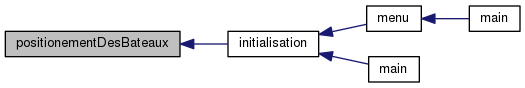
\includegraphics[width=350pt]{header_8h_a92c11248eb6a0ae0b0316938f3f07351_icgraph}
\end{center}
\end{figure}
\mbox{\Hypertarget{header_8h_aa7bd3bd80b4918740bf10a6b1fe3e57b}\label{header_8h_aa7bd3bd80b4918740bf10a6b1fe3e57b}} 
\index{header.\+h@{header.\+h}!print@{print}}
\index{print@{print}!header.\+h@{header.\+h}}
\subsubsection{\texorpdfstring{print()}{print()}}
{\footnotesize\ttfamily void print (\begin{DoxyParamCaption}\item[{\mbox{\hyperlink{structjoueur}{joueur}} $\ast$}]{player,  }\item[{int}]{c }\end{DoxyParamCaption})}



Une fonction qui affiche différent messager de mise en forme dasn le jeu a l\textquotesingle{}aide d\textquotesingle{}un int donner comme argument. 

Cette fonction permet d\textquotesingle{}afficher plusieur message d\textquotesingle{}indication selon la valeur de \char`\"{}int c\char`\"{}. 
\begin{DoxyParams}{Paramètres}
{\em joueur$\ast$} & player \+: le joueur. \\
\hline
{\em int} & cacher \+: une variable qui prend les valeurs 0, 1 , 2 et 3 . \\
\hline
\end{DoxyParams}


Définition à la ligne 99 du fichier affichage.\+c.



Références joueur\+::color, couleur, joueur\+::nom, R\+ED, et W\+H\+I\+TE.



Référencé par game\+Over(), jeu(), et jeu\+A\+N\+Coup().


\begin{DoxyCode}
99                                  \{
100     fflush(stdin);
101     \textcolor{keywordflow}{if}(c == 0)\{
102         \mbox{\hyperlink{header_8h_aabcb2d6536b6c0ab41f99493c911489b}{couleur}}(\mbox{\hyperlink{header_8h_a8d23feea868a983c8c2b661e1e16972f}{RED}}); printf(\textcolor{stringliteral}{"\%s, appyer sur entreé pour continuer!!\(\backslash\)n"}, player->
      \mbox{\hyperlink{structjoueur_a5228c842828b2639253cb7db01e6f72d}{nom}});
103         \mbox{\hyperlink{header_8h_aabcb2d6536b6c0ab41f99493c911489b}{couleur}}(\mbox{\hyperlink{header_8h_a87b537f5fa5c109d3c05c13d6b18f382}{WHITE}});
104         getchar();
105        CLEAR\_SCREEN;
106     \}\textcolor{keywordflow}{else} \textcolor{keywordflow}{if}(c == 1)\{
107         \mbox{\hyperlink{header_8h_aabcb2d6536b6c0ab41f99493c911489b}{couleur}}(\textcolor{stringliteral}{"47"}); \mbox{\hyperlink{header_8h_aabcb2d6536b6c0ab41f99493c911489b}{couleur}}(\mbox{\hyperlink{header_8h_a8d23feea868a983c8c2b661e1e16972f}{RED}});printf(\textcolor{stringliteral}{"\%s"},player->\mbox{\hyperlink{structjoueur_a5228c842828b2639253cb7db01e6f72d}{nom}});
108         printf(\textcolor{stringliteral}{", c'est ton tour de joue:\(\backslash\)n---------------------------\(\backslash\)n"});
109         \mbox{\hyperlink{header_8h_aabcb2d6536b6c0ab41f99493c911489b}{couleur}}(\mbox{\hyperlink{header_8h_a87b537f5fa5c109d3c05c13d6b18f382}{WHITE}});     
110     \}\textcolor{keywordflow}{else} \textcolor{keywordflow}{if}(c == 2)\{
111         printf(\textcolor{stringliteral}{"Le joueur "});
112         \mbox{\hyperlink{header_8h_aabcb2d6536b6c0ab41f99493c911489b}{couleur}}(player->\mbox{\hyperlink{structjoueur_a1064ba94d4d2719446f3c609135ba362}{color}});printf(\textcolor{stringliteral}{"\%s "},player->\mbox{\hyperlink{structjoueur_a5228c842828b2639253cb7db01e6f72d}{nom}});
113         \mbox{\hyperlink{header_8h_aabcb2d6536b6c0ab41f99493c911489b}{couleur}}(\mbox{\hyperlink{header_8h_a87b537f5fa5c109d3c05c13d6b18f382}{WHITE}});printf(\textcolor{stringliteral}{"à Gagner ^-^.\(\backslash\)n"});       
114         printf(\textcolor{stringliteral}{"La partie est terminer.\(\backslash\)nAppyer sur entreé pour revenir au menu principal!!"});
115         getchar();
116         CLEAR\_SCREEN;
117     \}\textcolor{keywordflow}{else} \textcolor{keywordflow}{if}(c == 3)\{
118         printf(\textcolor{stringliteral}{"La partie Va Commencer.\(\backslash\)nAppyer sur entreé pour continuer!!"});
119         getchar();
120         CLEAR\_SCREEN;
121     \}
122 \}
\end{DoxyCode}
Voici le graphe des appelants de cette fonction \+:\nopagebreak
\begin{figure}[H]
\begin{center}
\leavevmode
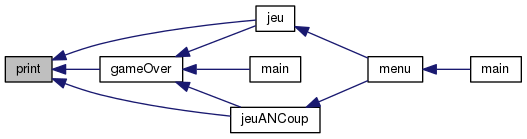
\includegraphics[width=350pt]{header_8h_aa7bd3bd80b4918740bf10a6b1fe3e57b_icgraph}
\end{center}
\end{figure}
\mbox{\Hypertarget{header_8h_a4bcd2f1cd82e9edd813bde29e9c12568}\label{header_8h_a4bcd2f1cd82e9edd813bde29e9c12568}} 
\index{header.\+h@{header.\+h}!table\+Board@{table\+Board}}
\index{table\+Board@{table\+Board}!header.\+h@{header.\+h}}
\subsubsection{\texorpdfstring{table\+Board()}{tableBoard()}}
{\footnotesize\ttfamily void table\+Board (\begin{DoxyParamCaption}\item[{\mbox{\hyperlink{structjoueur}{joueur}} $\ast$}]{player }\end{DoxyParamCaption})}



Une fonction qui affiche le resultat du joueur actuelle à chaque tour. 

Cette fonction permet d\textquotesingle{}afficher les resultats de chaque joueur a chaque tour de jeu. ~\newline

\begin{DoxyParams}{Paramètres}
{\em joueur$\ast$} & player \+: le joueur. \\
\hline
\end{DoxyParams}


Définition à la ligne 128 du fichier affichage.\+c.



Références joueur\+::bat, couleur, joueur\+::nbr\+\_\+bateau\+\_\+couler, joueur\+::nbr\+\_\+bateau\+\_\+restant, bateau\+::nbr\+\_\+case\+\_\+total, bateau\+::nbr\+\_\+case\+\_\+toucher, joueur\+::nbr\+\_\+tir\+\_\+manquer, joueur\+::nbr\+\_\+tir\+\_\+reussit, N\+O\+M\+B\+R\+E\+\_\+\+B\+A\+T\+E\+AU, et W\+H\+I\+TE.



Référencé par afficher().


\begin{DoxyCode}
128                                \{
129     \textcolor{keywordtype}{int} i;
130     player->\mbox{\hyperlink{structjoueur_ab0c0fa544d83148d4daed41c84954e55}{nbr\_bateau\_couler}} = 0;
131     \textcolor{keywordflow}{for} (i = 0; i < \mbox{\hyperlink{header_8h_a56aaacd8cb8ffd138094887b2d3344f6}{NOMBRE\_BATEAU}}; ++i)\{
132         \textcolor{keywordflow}{if}(player->\mbox{\hyperlink{structjoueur_a3b21aa14ce27f69126dc9a649b363146}{bat}}[i].\mbox{\hyperlink{structbateau_a62ae80832c521a9984c520fde88dadfd}{nbr\_case\_toucher}} == player->\mbox{\hyperlink{structjoueur_a3b21aa14ce27f69126dc9a649b363146}{bat}}[i].
      \mbox{\hyperlink{structbateau_aff445dc58a52069759f1e4bfd13c0313}{nbr\_case\_total}})\{
133             player->\mbox{\hyperlink{structjoueur_ab0c0fa544d83148d4daed41c84954e55}{nbr\_bateau\_couler}}++;
134             player->\mbox{\hyperlink{structjoueur_a4f902c486f8d66cb85cf3b07abd0bd12}{nbr\_bateau\_restant}} = \mbox{\hyperlink{header_8h_a56aaacd8cb8ffd138094887b2d3344f6}{NOMBRE\_BATEAU}} - player->
      \mbox{\hyperlink{structjoueur_ab0c0fa544d83148d4daed41c84954e55}{nbr\_bateau\_couler}};
135         \}
136     \}
137     \mbox{\hyperlink{header_8h_aabcb2d6536b6c0ab41f99493c911489b}{couleur}}(\textcolor{stringliteral}{"45"});
138     printf(\textcolor{stringliteral}{"Nombre de bateau restant : \%d   Nombre de bateau couler : \%d\(\backslash\)n"},player->
      \mbox{\hyperlink{structjoueur_a4f902c486f8d66cb85cf3b07abd0bd12}{nbr\_bateau\_restant}},player->\mbox{\hyperlink{structjoueur_ab0c0fa544d83148d4daed41c84954e55}{nbr\_bateau\_couler}});
139     printf(\textcolor{stringliteral}{"Nombre de tire reussi    : \%d   Nombre de tire manquer  : \%d\(\backslash\)n"},player->
      \mbox{\hyperlink{structjoueur_a19510a02b4ff3f6336da487b50806d71}{nbr\_tir\_reussit}},player->\mbox{\hyperlink{structjoueur_aaba095a23d03a15d363924e77caa3c1e}{nbr\_tir\_manquer}});
140     \mbox{\hyperlink{header_8h_aabcb2d6536b6c0ab41f99493c911489b}{couleur}}(\mbox{\hyperlink{header_8h_a87b537f5fa5c109d3c05c13d6b18f382}{WHITE}});
141 \}
\end{DoxyCode}
Voici le graphe des appelants de cette fonction \+:\nopagebreak
\begin{figure}[H]
\begin{center}
\leavevmode
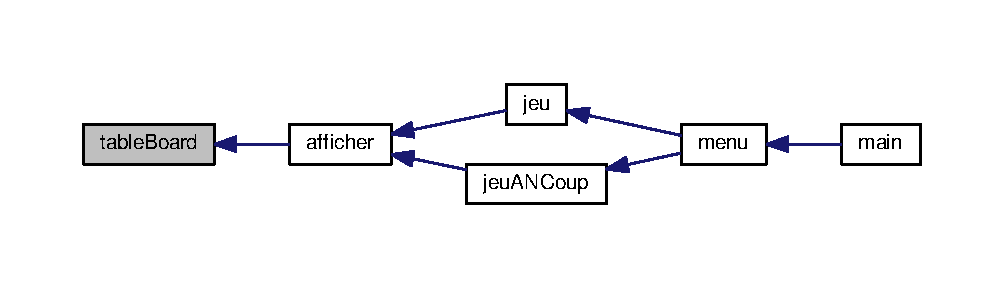
\includegraphics[width=350pt]{header_8h_a4bcd2f1cd82e9edd813bde29e9c12568_icgraph}
\end{center}
\end{figure}
\mbox{\Hypertarget{header_8h_a92241da559f8c98b3ec5a99f4d151658}\label{header_8h_a92241da559f8c98b3ec5a99f4d151658}} 
\index{header.\+h@{header.\+h}!tour@{tour}}
\index{tour@{tour}!header.\+h@{header.\+h}}
\subsubsection{\texorpdfstring{tour()}{tour()}}
{\footnotesize\ttfamily \mbox{\hyperlink{structjoueur}{joueur}}$\ast$ tour (\begin{DoxyParamCaption}\item[{\mbox{\hyperlink{structjoueur}{joueur}} $\ast$}]{player1,  }\item[{\mbox{\hyperlink{structjoueur}{joueur}} $\ast$}]{player2 }\end{DoxyParamCaption})}



Une fonction qui déroule le tour d\textquotesingle{}un jour. 

Cette fonction permet de jouer un tour. 
\begin{DoxyParams}{Paramètres}
{\em joueur$\ast$} & player1 \+: le joueur qui joue ~\newline
\\
\hline
{\em joueur$\ast$} & player2 \+: le joueur l\textquotesingle{}adversaire. ~\newline
\\
\hline
\end{DoxyParams}
\begin{DoxyReturn}{Renvoie}
Le joueur. 
\end{DoxyReturn}


Définition à la ligne 10 du fichier tour.\+c.



Références joueur\+::bat, joueur\+::ia, bateau\+::nbr\+\_\+case\+\_\+colonne, bateau\+::nbr\+\_\+case\+\_\+ligne, bateau\+::nbr\+\_\+case\+\_\+toucher, joueur\+::nbr\+\_\+tir\+\_\+manquer, joueur\+::nbr\+\_\+tir\+\_\+reussit, N\+O\+M\+B\+R\+E\+\_\+\+B\+A\+T\+E\+AU, joueur\+::plateau, bateau\+::position\+\_\+colonne, bateau\+::position\+\_\+ligne, et T\+A\+I\+L\+L\+E\+\_\+\+P\+L\+A\+T\+E\+AU.



Référencé par jeu(), jeu\+A\+N\+Coup(), et main().


\begin{DoxyCode}
10                                               \{
11   \textcolor{keywordtype}{int} ligne,colonne,occuper,i;
12 
13   \textcolor{keywordflow}{do}\{
14     occuper = 0;
15     \textcolor{comment}{// Obtenir le choix du joueur1 pour attaque une case  }
16     \textcolor{keywordflow}{if}(!player1->\mbox{\hyperlink{structjoueur_a307e3b4b4c1b78e753c599bc1f6a47c3}{ia}})\{
17       \textcolor{comment}{// Si le joueur1 est un humaine}
18       \textcolor{keywordflow}{do}\{
19           printf(\textcolor{stringliteral}{"(ligne,colonne) :"});
20           scanf(\textcolor{stringliteral}{"\%d \%d"},\&ligne,\&colonne);
21       \}\textcolor{keywordflow}{while}((ligne > \mbox{\hyperlink{header_8h_adc3c2556e84bebbe78c8a87fc459a6f8}{TAILLE\_PLATEAU}} || ligne < 0) || (colonne > 
      \mbox{\hyperlink{header_8h_adc3c2556e84bebbe78c8a87fc459a6f8}{TAILLE\_PLATEAU}} || colonne < 0));
22     \}\textcolor{keywordflow}{else}\{
23       \textcolor{comment}{// Si le joueur1 est une IA}
24       ligne = rand()\%\mbox{\hyperlink{header_8h_adc3c2556e84bebbe78c8a87fc459a6f8}{TAILLE\_PLATEAU}} + 1;
25       colonne = rand()\%\mbox{\hyperlink{header_8h_adc3c2556e84bebbe78c8a87fc459a6f8}{TAILLE\_PLATEAU}} + 1;
26     \}
27     \textcolor{comment}{// Savoir quelle case est touché celle d'un bateau ou une case vide ou une deja joue précdament }
28     \textcolor{keywordflow}{if}(player2->\mbox{\hyperlink{structjoueur_a0de66c3578a57ff8e0ed1bf3d91c8e82}{plateau}}[ligne - 1][colonne - 1] == \textcolor{charliteral}{'\#'})\{
29       \textcolor{comment}{//bateau toucher incrémentation du nombre de tire réussi}
30       player2->\mbox{\hyperlink{structjoueur_a0de66c3578a57ff8e0ed1bf3d91c8e82}{plateau}}[ligne - 1][colonne - 1] = \textcolor{charliteral}{'X'};
31       player1->\mbox{\hyperlink{structjoueur_a19510a02b4ff3f6336da487b50806d71}{nbr\_tir\_reussit}}++;
32       \textcolor{comment}{// Savoir quelle bateau est toucher est incrémenter le nombre de case toucher pour ce bateau }
33       \textcolor{keywordflow}{for} (i = 0; i < \mbox{\hyperlink{header_8h_a56aaacd8cb8ffd138094887b2d3344f6}{NOMBRE\_BATEAU}}; ++i)\{
34         \textcolor{keywordflow}{if}(((colonne - 1 >= player2-> \mbox{\hyperlink{structjoueur_a3b21aa14ce27f69126dc9a649b363146}{bat}}[i].\mbox{\hyperlink{structbateau_aac775edde7cde57176e580c29f6e8eca}{position\_colonne}})
35             \&\& (colonne - 1 < player2-> \mbox{\hyperlink{structjoueur_a3b21aa14ce27f69126dc9a649b363146}{bat}}[i].\mbox{\hyperlink{structbateau_aac775edde7cde57176e580c29f6e8eca}{position\_colonne}} + player2-> 
      \mbox{\hyperlink{structjoueur_a3b21aa14ce27f69126dc9a649b363146}{bat}}[i].\mbox{\hyperlink{structbateau_a1a56dd379e7c5cfc5714fd204947a0a8}{nbr\_case\_colonne}})) \&\&
36             ((ligne - 1 >= player2-> \mbox{\hyperlink{structjoueur_a3b21aa14ce27f69126dc9a649b363146}{bat}}[i].\mbox{\hyperlink{structbateau_a5dcd33e534b9b1b8b0414325bc5c09b1}{position\_ligne}})
37             \&\& (ligne  - 1< player2-> \mbox{\hyperlink{structjoueur_a3b21aa14ce27f69126dc9a649b363146}{bat}}[i].\mbox{\hyperlink{structbateau_a5dcd33e534b9b1b8b0414325bc5c09b1}{position\_ligne}} + player2->
      \mbox{\hyperlink{structjoueur_a3b21aa14ce27f69126dc9a649b363146}{bat}}[i].\mbox{\hyperlink{structbateau_a5f7637b2932717e5589e1a368dd1b47b}{nbr\_case\_ligne}})))\{
38           player2->\mbox{\hyperlink{structjoueur_a3b21aa14ce27f69126dc9a649b363146}{bat}}[i].\mbox{\hyperlink{structbateau_a62ae80832c521a9984c520fde88dadfd}{nbr\_case\_toucher}}++;
39           \textcolor{keywordflow}{break};
40         \}
41       \}
42     \}
43     \textcolor{keywordflow}{else}\{
44       \textcolor{keywordflow}{if} (player2->\mbox{\hyperlink{structjoueur_a0de66c3578a57ff8e0ed1bf3d91c8e82}{plateau}}[ligne - 1][colonne - 1] == \textcolor{charliteral}{'X'} || player2->
      \mbox{\hyperlink{structjoueur_a0de66c3578a57ff8e0ed1bf3d91c8e82}{plateau}}[ligne - 1][colonne - 1] == \textcolor{charliteral}{'O'} )
45         occuper = 1;\textcolor{comment}{// Case précédament toucher }
46       \textcolor{keywordflow}{else}\{
47         \textcolor{comment}{// case vide toucher incréménter le nombre de tir manger}
48         player2->\mbox{\hyperlink{structjoueur_a0de66c3578a57ff8e0ed1bf3d91c8e82}{plateau}}[ligne - 1][colonne - 1] = \textcolor{charliteral}{'O'};
49         player1->\mbox{\hyperlink{structjoueur_aaba095a23d03a15d363924e77caa3c1e}{nbr\_tir\_manquer}}++;
50       \}
51     \}
52   \}\textcolor{keywordflow}{while}(occuper == 1);
53 
54   \textcolor{keywordflow}{return} player2;
55 \}
\end{DoxyCode}
Voici le graphe des appelants de cette fonction \+:\nopagebreak
\begin{figure}[H]
\begin{center}
\leavevmode
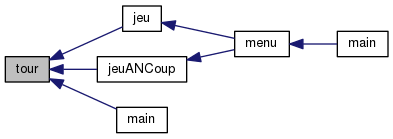
\includegraphics[width=350pt]{header_8h_a92241da559f8c98b3ec5a99f4d151658_icgraph}
\end{center}
\end{figure}

\hypertarget{initialisation_8c}{}\section{Référence du fichier initialisation.\+c}
\label{initialisation_8c}\index{initialisation.\+c@{initialisation.\+c}}
{\ttfamily \#include \char`\"{}header.\+h\char`\"{}}\newline
Graphe des dépendances par inclusion de initialisation.\+c\+:\nopagebreak
\begin{figure}[H]
\begin{center}
\leavevmode
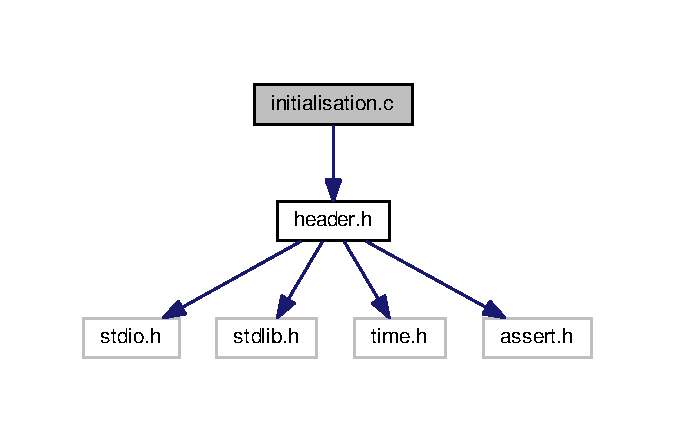
\includegraphics[width=324pt]{initialisation_8c__incl}
\end{center}
\end{figure}
\subsection*{Fonctions}
\begin{DoxyCompactItemize}
\item 
\mbox{\hyperlink{structjoueur}{joueur}} $\ast$ \mbox{\hyperlink{initialisation_8c_a0b7a5f024d081c47696bf97c89a367f7}{initialisation}} (\mbox{\hyperlink{structjoueur}{joueur}} $\ast$player, char $\ast$color, int ia)
\begin{DoxyCompactList}\small\item\em Une fonction qui fait l\textquotesingle{}initialisation de chaque joueur au début du jeu. \end{DoxyCompactList}\end{DoxyCompactItemize}


\subsection{Description détaillée}
\begin{DoxyAuthor}{Auteur}
B.\+Habib, A.\+Sofiane, I.\+Tinhinane, I.\+Chafia 
\end{DoxyAuthor}
\begin{DoxyVersion}{Version}
1.\+0 
\end{DoxyVersion}
\begin{DoxyDate}{Date}
07 Avril 2018
\end{DoxyDate}
définition de la fonction initialisation 

\subsection{Documentation des fonctions}
\mbox{\Hypertarget{initialisation_8c_a0b7a5f024d081c47696bf97c89a367f7}\label{initialisation_8c_a0b7a5f024d081c47696bf97c89a367f7}} 
\index{initialisation.\+c@{initialisation.\+c}!initialisation@{initialisation}}
\index{initialisation@{initialisation}!initialisation.\+c@{initialisation.\+c}}
\subsubsection{\texorpdfstring{initialisation()}{initialisation()}}
{\footnotesize\ttfamily \mbox{\hyperlink{structjoueur}{joueur}}$\ast$ initialisation (\begin{DoxyParamCaption}\item[{\mbox{\hyperlink{structjoueur}{joueur}} $\ast$}]{player,  }\item[{char $\ast$}]{color,  }\item[{int}]{ia }\end{DoxyParamCaption})}



Une fonction qui fait l\textquotesingle{}initialisation de chaque joueur au début du jeu. 

Cette fonction permet d\textquotesingle{}intialiser les champ du joueur passer en argument. 
\begin{DoxyParams}{Paramètres}
{\em joueur$\ast$} & player \+: le joueur. \\
\hline
{\em char$\ast$} & color \+: la couleur par défaut du joueur. \\
\hline
{\em int} & ia \+: une valeur qui indique la nature du joueur humaine ou ia. \\
\hline
\end{DoxyParams}
\begin{DoxyReturn}{Renvoie}
le joueur. 
\end{DoxyReturn}


Définition à la ligne 10 du fichier initialisation.\+c.



Références joueur\+::color, joueur\+::ia, joueur\+::nbr\+\_\+bateau\+\_\+couler, joueur\+::nbr\+\_\+bateau\+\_\+restant, joueur\+::nbr\+\_\+tir\+\_\+manquer, joueur\+::nbr\+\_\+tir\+\_\+reussit, joueur\+::nom, N\+O\+M\+B\+R\+E\+\_\+\+B\+A\+T\+E\+AU, joueur\+::plateau, positionement\+Des\+Bateaux(), et T\+A\+I\+L\+L\+E\+\_\+\+P\+L\+A\+T\+E\+AU.



Référencé par main(), et menu().


\begin{DoxyCode}
10                                                            \{
11     \textcolor{keywordtype}{int} ligne, colonne;
12     player = malloc(\textcolor{keyword}{sizeof} (*player));
13     printf(\textcolor{stringliteral}{"Donner Le  Nom Du Joueur:"});
14     player->\mbox{\hyperlink{structjoueur_a5228c842828b2639253cb7db01e6f72d}{nom}} = malloc(10 * \textcolor{keyword}{sizeof}(\textcolor{keywordtype}{char}));
15     scanf(\textcolor{stringliteral}{"\%s"},player->\mbox{\hyperlink{structjoueur_a5228c842828b2639253cb7db01e6f72d}{nom}});
16     
17     \textcolor{keywordflow}{for}(ligne = 0 ; ligne < \mbox{\hyperlink{header_8h_adc3c2556e84bebbe78c8a87fc459a6f8}{TAILLE\_PLATEAU}} ; ++ligne)
18         \textcolor{keywordflow}{for}(colonne = 0 ; colonne < \mbox{\hyperlink{header_8h_adc3c2556e84bebbe78c8a87fc459a6f8}{TAILLE\_PLATEAU}} ; ++colonne)
19             player->\mbox{\hyperlink{structjoueur_a0de66c3578a57ff8e0ed1bf3d91c8e82}{plateau}}[ligne][colonne] = \textcolor{charliteral}{' '};
20 
21     player->\mbox{\hyperlink{structjoueur_a307e3b4b4c1b78e753c599bc1f6a47c3}{ia}} = \mbox{\hyperlink{structjoueur_a307e3b4b4c1b78e753c599bc1f6a47c3}{ia}};
22     player->\mbox{\hyperlink{structjoueur_ab0c0fa544d83148d4daed41c84954e55}{nbr\_bateau\_couler}} = 0;
23     player->\mbox{\hyperlink{structjoueur_a4f902c486f8d66cb85cf3b07abd0bd12}{nbr\_bateau\_restant}} = \mbox{\hyperlink{header_8h_a56aaacd8cb8ffd138094887b2d3344f6}{NOMBRE\_BATEAU}};
24     player->\mbox{\hyperlink{structjoueur_a19510a02b4ff3f6336da487b50806d71}{nbr\_tir\_reussit}} = 0;
25     player->\mbox{\hyperlink{structjoueur_aaba095a23d03a15d363924e77caa3c1e}{nbr\_tir\_manquer}} = 0;
26     player->\mbox{\hyperlink{structjoueur_a1064ba94d4d2719446f3c609135ba362}{color}} = \mbox{\hyperlink{structjoueur_a1064ba94d4d2719446f3c609135ba362}{color}};
27     
28     player = \mbox{\hyperlink{header_8h_a92c11248eb6a0ae0b0316938f3f07351}{positionementDesBateaux}}(player);
29     \textcolor{keywordflow}{return} player;
30 \}
\end{DoxyCode}
Voici le graphe d\textquotesingle{}appel pour cette fonction \+:\nopagebreak
\begin{figure}[H]
\begin{center}
\leavevmode
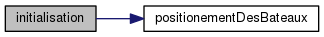
\includegraphics[width=315pt]{initialisation_8c_a0b7a5f024d081c47696bf97c89a367f7_cgraph}
\end{center}
\end{figure}
Voici le graphe des appelants de cette fonction \+:\nopagebreak
\begin{figure}[H]
\begin{center}
\leavevmode
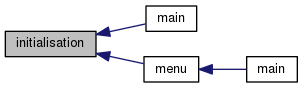
\includegraphics[width=299pt]{initialisation_8c_a0b7a5f024d081c47696bf97c89a367f7_icgraph}
\end{center}
\end{figure}

\hypertarget{jeux_8c}{}\section{Référence du fichier jeux.\+c}
\label{jeux_8c}\index{jeux.\+c@{jeux.\+c}}
{\ttfamily \#include \char`\"{}header.\+h\char`\"{}}\newline
Graphe des dépendances par inclusion de jeux.\+c\+:\nopagebreak
\begin{figure}[H]
\begin{center}
\leavevmode
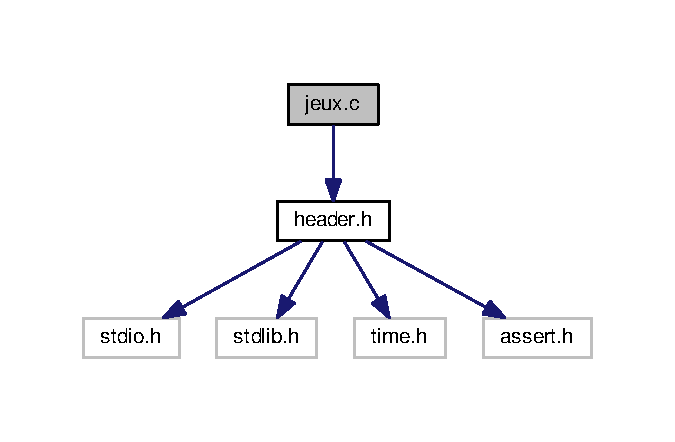
\includegraphics[width=324pt]{jeux_8c__incl}
\end{center}
\end{figure}
\subsection*{Fonctions}
\begin{DoxyCompactItemize}
\item 
int \mbox{\hyperlink{jeux_8c_a3610cb607e2029a8583ce054be882fbc}{game\+Over}} (\mbox{\hyperlink{structjoueur}{joueur}} $\ast$player)
\begin{DoxyCompactList}\small\item\em Une fonction qui vérifier la fin du jeu. \end{DoxyCompactList}\item 
void \mbox{\hyperlink{jeux_8c_a740a3255999f6e89a7a7d6fc7a045caa}{jeu}} (\mbox{\hyperlink{structjoueur}{joueur}} $\ast$player1, \mbox{\hyperlink{structjoueur}{joueur}} $\ast$player2)
\begin{DoxyCompactList}\small\item\em Une fonction qui déroule le jeu. \end{DoxyCompactList}\item 
void \mbox{\hyperlink{jeux_8c_a08ee89b1bab3612448b36d13faab6fa8}{jeu\+A\+N\+Coup}} (\mbox{\hyperlink{structjoueur}{joueur}} $\ast$player1, \mbox{\hyperlink{structjoueur}{joueur}} $\ast$player2, int n)
\begin{DoxyCompactList}\small\item\em une fonction qui déroule jeu avancer de N coupe simuler \end{DoxyCompactList}\end{DoxyCompactItemize}


\subsection{Documentation des fonctions}
\mbox{\Hypertarget{jeux_8c_a3610cb607e2029a8583ce054be882fbc}\label{jeux_8c_a3610cb607e2029a8583ce054be882fbc}} 
\index{jeux.\+c@{jeux.\+c}!game\+Over@{game\+Over}}
\index{game\+Over@{game\+Over}!jeux.\+c@{jeux.\+c}}
\subsubsection{\texorpdfstring{game\+Over()}{gameOver()}}
{\footnotesize\ttfamily int game\+Over (\begin{DoxyParamCaption}\item[{\mbox{\hyperlink{structjoueur}{joueur}} $\ast$}]{player }\end{DoxyParamCaption})}



Une fonction qui vérifier la fin du jeu. 

Cette fonction permet de savoir la fin du jeu en testent l\textquotesingle{}égaliter entre le nombre de tir reussit et le nombre de case total pour l\textquotesingle{}ensemble des bateaux ~\newline

\begin{DoxyParams}{Paramètres}
{\em joueur$\ast$} & player \+: le joueur concerner. \\
\hline
\end{DoxyParams}


Définition à la ligne 8 du fichier jeux.\+c.



Références joueur\+::nbr\+\_\+tir\+\_\+reussit, N\+O\+M\+B\+R\+E\+\_\+\+C\+A\+S\+E\+\_\+\+B\+A\+T\+E\+AU, et print().



Référencé par jeu(), jeu\+A\+N\+Coup(), et main().


\begin{DoxyCode}
8                             \{
9   \textcolor{keywordflow}{if}(player->\mbox{\hyperlink{structjoueur_a19510a02b4ff3f6336da487b50806d71}{nbr\_tir\_reussit}} == \mbox{\hyperlink{header_8h_a491086a202f32f357e418a99cde7156e}{NOMBRE\_CASE\_BATEAU}})\{
10     \mbox{\hyperlink{affichage_8c_a34b6e28e00a180632a300b9608ad6acd}{print}}(player, 2);
11     \textcolor{keywordflow}{return} 1;
12   \}
13   \textcolor{keywordflow}{else} 
14     \textcolor{keywordflow}{return} 0; 
15 \}
\end{DoxyCode}
Voici le graphe d\textquotesingle{}appel pour cette fonction \+:\nopagebreak
\begin{figure}[H]
\begin{center}
\leavevmode
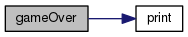
\includegraphics[width=213pt]{jeux_8c_a3610cb607e2029a8583ce054be882fbc_cgraph}
\end{center}
\end{figure}
Voici le graphe des appelants de cette fonction \+:\nopagebreak
\begin{figure}[H]
\begin{center}
\leavevmode
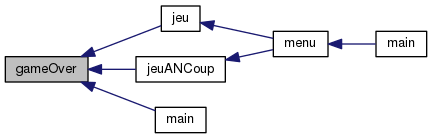
\includegraphics[width=350pt]{jeux_8c_a3610cb607e2029a8583ce054be882fbc_icgraph}
\end{center}
\end{figure}
\mbox{\Hypertarget{jeux_8c_a740a3255999f6e89a7a7d6fc7a045caa}\label{jeux_8c_a740a3255999f6e89a7a7d6fc7a045caa}} 
\index{jeux.\+c@{jeux.\+c}!jeu@{jeu}}
\index{jeu@{jeu}!jeux.\+c@{jeux.\+c}}
\subsubsection{\texorpdfstring{jeu()}{jeu()}}
{\footnotesize\ttfamily void jeu (\begin{DoxyParamCaption}\item[{\mbox{\hyperlink{structjoueur}{joueur}} $\ast$}]{player1,  }\item[{\mbox{\hyperlink{structjoueur}{joueur}} $\ast$}]{player2 }\end{DoxyParamCaption})}



Une fonction qui déroule le jeu. 

Cette fonction permet de jouer à une partie du jeu. 
\begin{DoxyParams}{Paramètres}
{\em joueur$\ast$} & player1 \+: le joueur 1. \\
\hline
{\em joueur$\ast$} & player2 \+: le joueur 2. \\
\hline
\end{DoxyParams}


Définition à la ligne 22 du fichier jeux.\+c.



Références afficher(), game\+Over(), joueur\+::ia, print(), et tour().



Référencé par menu().


\begin{DoxyCode}
22                                          \{
23   \mbox{\hyperlink{structjoueur}{joueur}}* joueurActualle;
24   \textcolor{keywordtype}{int} i = 0;
25     
26   joueurActualle = player1;
27   \mbox{\hyperlink{affichage_8c_a34b6e28e00a180632a300b9608ad6acd}{print}}(joueurActualle,3);
28   \textcolor{keywordflow}{while}(!\mbox{\hyperlink{jeux_8c_a3610cb607e2029a8583ce054be882fbc}{gameOver}}(joueurActualle))\{
29   \textcolor{comment}{// Le joueur 1 jeu son tour}
30     joueurActualle = player1;
31     \textcolor{keywordflow}{if}(player1->\mbox{\hyperlink{structjoueur_a307e3b4b4c1b78e753c599bc1f6a47c3}{ia}} == player2->\mbox{\hyperlink{structjoueur_a307e3b4b4c1b78e753c599bc1f6a47c3}{ia}})\{
32       \mbox{\hyperlink{affichage_8c_a34b6e28e00a180632a300b9608ad6acd}{print}}(joueurActualle, 1);
33       \mbox{\hyperlink{affichage_8c_a8004c5a076f6d53e90583b921ac810cb}{afficher}}(player2, player1,1);
34     \}
35     \textcolor{comment}{// Le joueur 1 choisit une case du plateau du joueur 2 }
36     player2 = \mbox{\hyperlink{header_8h_a92241da559f8c98b3ec5a99f4d151658}{tour}}(player1, player2);
37     \textcolor{keywordflow}{if}(player1->\mbox{\hyperlink{structjoueur_a307e3b4b4c1b78e753c599bc1f6a47c3}{ia}} == player2->\mbox{\hyperlink{structjoueur_a307e3b4b4c1b78e753c599bc1f6a47c3}{ia}}) \mbox{\hyperlink{affichage_8c_a34b6e28e00a180632a300b9608ad6acd}{print}}(joueurActualle, 0);
38     \textcolor{comment}{//On teste c'est le joueur 1  à gagner}
39     \textcolor{keywordflow}{if}(!\mbox{\hyperlink{jeux_8c_a3610cb607e2029a8583ce054be882fbc}{gameOver}}(joueurActualle))\{
40     \textcolor{comment}{// Le joueur 2 jeu son tour}
41       joueurActualle = player2;
42       \mbox{\hyperlink{affichage_8c_a34b6e28e00a180632a300b9608ad6acd}{print}}(joueurActualle, 1);  
43       \mbox{\hyperlink{affichage_8c_a8004c5a076f6d53e90583b921ac810cb}{afficher}}(player1, player2,1);
44       \textcolor{comment}{// Le joueur 2 choisit une case du plateau du joueur 1}
45       player1 = \mbox{\hyperlink{header_8h_a92241da559f8c98b3ec5a99f4d151658}{tour}}(player2, player1);      
46       \mbox{\hyperlink{affichage_8c_a34b6e28e00a180632a300b9608ad6acd}{print}}(joueurActualle, 0);
47     \}\textcolor{keywordflow}{else}\{
48       \textcolor{keywordflow}{break};
49     \}
50     i++;
51   \}
52   printf(\textcolor{stringliteral}{"Le nombre de tour joue = \%d\(\backslash\)n"},i);
53 \}
\end{DoxyCode}
Voici le graphe d\textquotesingle{}appel pour cette fonction \+:\nopagebreak
\begin{figure}[H]
\begin{center}
\leavevmode
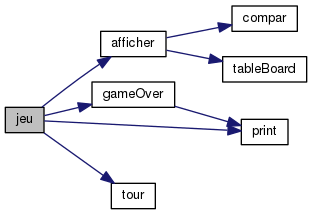
\includegraphics[width=306pt]{jeux_8c_a740a3255999f6e89a7a7d6fc7a045caa_cgraph}
\end{center}
\end{figure}
Voici le graphe des appelants de cette fonction \+:\nopagebreak
\begin{figure}[H]
\begin{center}
\leavevmode
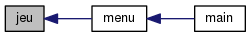
\includegraphics[width=260pt]{jeux_8c_a740a3255999f6e89a7a7d6fc7a045caa_icgraph}
\end{center}
\end{figure}
\mbox{\Hypertarget{jeux_8c_a08ee89b1bab3612448b36d13faab6fa8}\label{jeux_8c_a08ee89b1bab3612448b36d13faab6fa8}} 
\index{jeux.\+c@{jeux.\+c}!jeu\+A\+N\+Coup@{jeu\+A\+N\+Coup}}
\index{jeu\+A\+N\+Coup@{jeu\+A\+N\+Coup}!jeux.\+c@{jeux.\+c}}
\subsubsection{\texorpdfstring{jeu\+A\+N\+Coup()}{jeuANCoup()}}
{\footnotesize\ttfamily void jeu\+A\+N\+Coup (\begin{DoxyParamCaption}\item[{\mbox{\hyperlink{structjoueur}{joueur}} $\ast$}]{player1,  }\item[{\mbox{\hyperlink{structjoueur}{joueur}} $\ast$}]{player2,  }\item[{int}]{n }\end{DoxyParamCaption})}



une fonction qui déroule jeu avancer de N coupe simuler 

Cette fonction permet d\textquotesingle{}avancer la parti à un coup. 
\begin{DoxyParams}{Paramètres}
{\em joueur$\ast$} & player1 \+: le joueur 1. \\
\hline
{\em joueur$\ast$} & player2 \+: le joueur 2. \\
\hline
{\em int} & n \+: le nombre de tour que on veut avancé le jeu. \\
\hline
\end{DoxyParams}


Définition à la ligne 61 du fichier jeux.\+c.



Références afficher(), game\+Over(), joueur\+::ia, print(), et tour().



Référencé par menu().


\begin{DoxyCode}
61                                                      \{
62   \mbox{\hyperlink{structjoueur}{joueur}}* joueurActualle = player1;
63   \textcolor{keywordtype}{int} i = 0, ia1 = player1->\mbox{\hyperlink{structjoueur_a307e3b4b4c1b78e753c599bc1f6a47c3}{ia}}, ia2 = player2->\mbox{\hyperlink{structjoueur_a307e3b4b4c1b78e753c599bc1f6a47c3}{ia}};
64 
65   \mbox{\hyperlink{affichage_8c_a34b6e28e00a180632a300b9608ad6acd}{print}}(joueurActualle,3);
66   player1->\mbox{\hyperlink{structjoueur_a307e3b4b4c1b78e753c599bc1f6a47c3}{ia}} = 1;
67   player2->\mbox{\hyperlink{structjoueur_a307e3b4b4c1b78e753c599bc1f6a47c3}{ia}} = 1;
68   \textcolor{keywordflow}{while}(!\mbox{\hyperlink{jeux_8c_a3610cb607e2029a8583ce054be882fbc}{gameOver}}(joueurActualle) \&\& (i < n))\{
69     joueurActualle = player1;
70     player2 = \mbox{\hyperlink{header_8h_a92241da559f8c98b3ec5a99f4d151658}{tour}}(player1, player2);
71     \textcolor{keywordflow}{if}(!\mbox{\hyperlink{jeux_8c_a3610cb607e2029a8583ce054be882fbc}{gameOver}}(joueurActualle))\{
72       joueurActualle = player2;
73       player1 = \mbox{\hyperlink{header_8h_a92241da559f8c98b3ec5a99f4d151658}{tour}}(player2, player1);
74     \}
75     i++;
76   \}
77   player1->\mbox{\hyperlink{structjoueur_a307e3b4b4c1b78e753c599bc1f6a47c3}{ia}} = ia1;
78   player2->\mbox{\hyperlink{structjoueur_a307e3b4b4c1b78e753c599bc1f6a47c3}{ia}} = ia2;
79   \textcolor{keywordflow}{while}(!\mbox{\hyperlink{jeux_8c_a3610cb607e2029a8583ce054be882fbc}{gameOver}}(joueurActualle))\{
80     joueurActualle = player1;
81     \mbox{\hyperlink{affichage_8c_a34b6e28e00a180632a300b9608ad6acd}{print}}(joueurActualle, 1);
82     \mbox{\hyperlink{affichage_8c_a8004c5a076f6d53e90583b921ac810cb}{afficher}}(player2, player1, 1);
83     player2 = \mbox{\hyperlink{header_8h_a92241da559f8c98b3ec5a99f4d151658}{tour}}(player1, player2);
84     \mbox{\hyperlink{affichage_8c_a34b6e28e00a180632a300b9608ad6acd}{print}}(player2, 0);
85 
86     \textcolor{keywordflow}{if}(!\mbox{\hyperlink{jeux_8c_a3610cb607e2029a8583ce054be882fbc}{gameOver}}(joueurActualle))\{
87       joueurActualle = player2;
88       \mbox{\hyperlink{affichage_8c_a34b6e28e00a180632a300b9608ad6acd}{print}}(joueurActualle, 1);
89       \mbox{\hyperlink{affichage_8c_a8004c5a076f6d53e90583b921ac810cb}{afficher}}(player1, player2, 1);
90       player1 = \mbox{\hyperlink{header_8h_a92241da559f8c98b3ec5a99f4d151658}{tour}}(player2, player1);
91       \mbox{\hyperlink{affichage_8c_a34b6e28e00a180632a300b9608ad6acd}{print}}(player2, 0);
92     \}\textcolor{keywordflow}{else} 
93       \textcolor{keywordflow}{break};
94     i++;
95   \}
96   printf(\textcolor{stringliteral}{"Le nombre de tour joue = \%d\(\backslash\)n"},i);
97 \}
\end{DoxyCode}
Voici le graphe d\textquotesingle{}appel pour cette fonction \+:\nopagebreak
\begin{figure}[H]
\begin{center}
\leavevmode
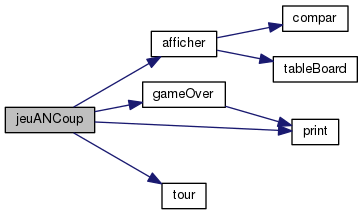
\includegraphics[width=344pt]{jeux_8c_a08ee89b1bab3612448b36d13faab6fa8_cgraph}
\end{center}
\end{figure}
Voici le graphe des appelants de cette fonction \+:\nopagebreak
\begin{figure}[H]
\begin{center}
\leavevmode
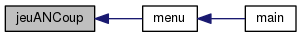
\includegraphics[width=298pt]{jeux_8c_a08ee89b1bab3612448b36d13faab6fa8_icgraph}
\end{center}
\end{figure}

\hypertarget{main_8c}{}\section{Référence du fichier main.\+c}
\label{main_8c}\index{main.\+c@{main.\+c}}
{\ttfamily \#include \char`\"{}header.\+h\char`\"{}}\newline
Graphe des dépendances par inclusion de main.\+c\+:\nopagebreak
\begin{figure}[H]
\begin{center}
\leavevmode
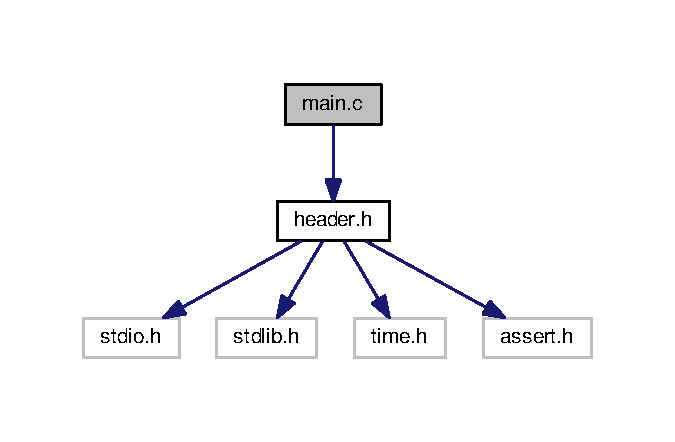
\includegraphics[width=324pt]{main_8c__incl}
\end{center}
\end{figure}
\subsection*{Fonctions}
\begin{DoxyCompactItemize}
\item 
int \mbox{\hyperlink{main_8c_ae66f6b31b5ad750f1fe042a706a4e3d4}{main}} ()
\end{DoxyCompactItemize}


\subsection{Documentation des fonctions}
\mbox{\Hypertarget{main_8c_ae66f6b31b5ad750f1fe042a706a4e3d4}\label{main_8c_ae66f6b31b5ad750f1fe042a706a4e3d4}} 
\index{main.\+c@{main.\+c}!main@{main}}
\index{main@{main}!main.\+c@{main.\+c}}
\subsubsection{\texorpdfstring{main()}{main()}}
{\footnotesize\ttfamily int main (\begin{DoxyParamCaption}\item[{void}]{ }\end{DoxyParamCaption})}



Définition à la ligne 3 du fichier main.\+c.



Références menu().


\begin{DoxyCode}
3           \{
4     \mbox{\hyperlink{header_8h_a2a0e843767aeea4f433a28b9c54f573a}{menu}}();
5 \textcolor{keywordflow}{return} 0;
6 \}
\end{DoxyCode}
Voici le graphe d\textquotesingle{}appel pour cette fonction \+:\nopagebreak
\begin{figure}[H]
\begin{center}
\leavevmode
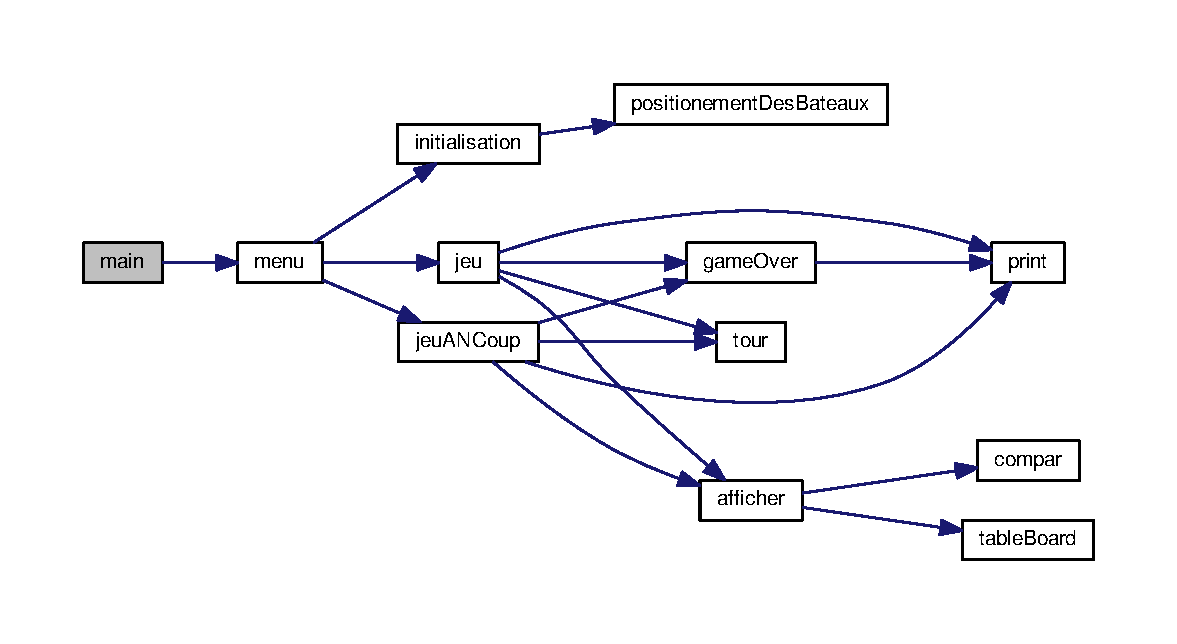
\includegraphics[width=350pt]{main_8c_ae66f6b31b5ad750f1fe042a706a4e3d4_cgraph}
\end{center}
\end{figure}

\hypertarget{menu_8c}{}\section{Référence du fichier menu.\+c}
\label{menu_8c}\index{menu.\+c@{menu.\+c}}
{\ttfamily \#include \char`\"{}header.\+h\char`\"{}}\newline
Graphe des dépendances par inclusion de menu.\+c\+:\nopagebreak
\begin{figure}[H]
\begin{center}
\leavevmode
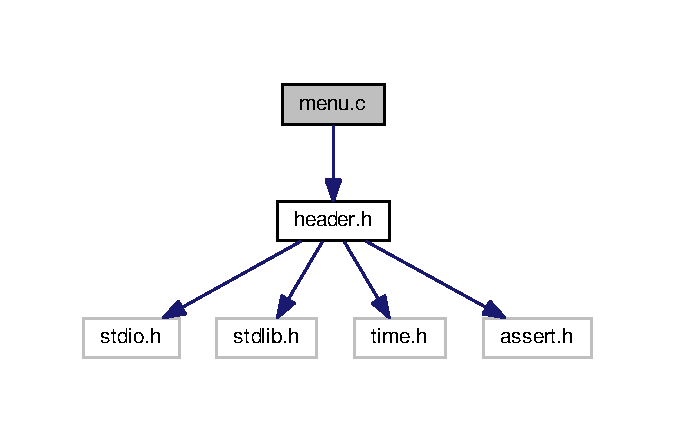
\includegraphics[width=324pt]{menu_8c__incl}
\end{center}
\end{figure}
\subsection*{Fonctions}
\begin{DoxyCompactItemize}
\item 
void \mbox{\hyperlink{menu_8c_a2a0e843767aeea4f433a28b9c54f573a}{menu}} ()
\begin{DoxyCompactList}\small\item\em Une fonction qui affiche le menu du jeu. \end{DoxyCompactList}\end{DoxyCompactItemize}


\subsection{Description détaillée}
\begin{DoxyAuthor}{Auteur}
B.\+Habib, A.\+Sofiane, I.\+Tinhinane, I.\+Chafia 
\end{DoxyAuthor}
\begin{DoxyVersion}{Version}
1.\+0 
\end{DoxyVersion}
\begin{DoxyDate}{Date}
07 Avril 2018
\end{DoxyDate}
définition de a fonction menu 

\subsection{Documentation des fonctions}
\mbox{\Hypertarget{menu_8c_a2a0e843767aeea4f433a28b9c54f573a}\label{menu_8c_a2a0e843767aeea4f433a28b9c54f573a}} 
\index{menu.\+c@{menu.\+c}!menu@{menu}}
\index{menu@{menu}!menu.\+c@{menu.\+c}}
\subsubsection{\texorpdfstring{menu()}{menu()}}
{\footnotesize\ttfamily void menu (\begin{DoxyParamCaption}{ }\end{DoxyParamCaption})}



Une fonction qui affiche le menu du jeu. 

Cette fonction permet d\textquotesingle{}afficher le menu principale du jeu. 

Définition à la ligne 6 du fichier menu.\+c.



Références G\+R\+E\+EN, initialisation(), jeu(), jeu\+A\+N\+Coup(), et Y\+E\+L\+L\+OW.



Référencé par main().


\begin{DoxyCode}
6            \{
7 srand(time(NULL));
8 \mbox{\hyperlink{structjoueur}{joueur}}* joueur1;
9 \mbox{\hyperlink{structjoueur}{joueur}}* joueur2;
10 \textcolor{keywordtype}{int} choix,n;
11 \textcolor{keywordflow}{do}\{
12   CLEAR\_SCREEN;
13   printf(\textcolor{stringliteral}{"\(\backslash\)t\(\backslash\)t\(\backslash\)033[42mBATAILLE NAVALE\(\backslash\)033[0m\(\backslash\)n"});
14   printf(\textcolor{stringliteral}{"\(\backslash\)033[35m----------------------------------------------------------\(\backslash\)n"});
15   printf(\textcolor{stringliteral}{"\(\backslash\)033[35m|\(\backslash\)033[33m1-\(\backslash\)033[32mPartie :\(\backslash\)033[34m Humain vs Humain\(\backslash\)033[37m                           \(\backslash\)0
      33[35m|\(\backslash\)n"});
16   printf(\textcolor{stringliteral}{"\(\backslash\)033[35m|\(\backslash\)033[33m2-\(\backslash\)033[32mPartie :\(\backslash\)033[34m Ordi vs Ordi\(\backslash\)033[37m                         \(\backslash\)0
      33[35m|\(\backslash\)n"});
17   printf(\textcolor{stringliteral}{"\(\backslash\)033[35m|\(\backslash\)033[33m3-\(\backslash\)033[32mPartie :\(\backslash\)033[34m Humain vs Ordi\(\backslash\)033[37m                         \(\backslash\)0
      33[35m|\(\backslash\)n"});
18   printf(\textcolor{stringliteral}{"\(\backslash\)033[35m|\(\backslash\)033[33m4-\(\backslash\)033[32mPartie :\(\backslash\)033[34m Humain vs Humain Partier Avancer de n coupe\(\backslash\)033[37m  
      \(\backslash\)033[35m|\(\backslash\)n"});
19   printf(\textcolor{stringliteral}{"\(\backslash\)033[35m|\(\backslash\)033[33m5-\(\backslash\)033[31mQuitter                                               \(\backslash\)033[35m|\(\backslash\)n"});
20   printf(\textcolor{stringliteral}{"----------------------------------------------------------\(\backslash\)n"});
21   printf(\textcolor{stringliteral}{"\(\backslash\)033[37mChoisir Dans Le Menu :"});
22 
23   \textcolor{keywordflow}{do} \{
24     scanf(\textcolor{stringliteral}{"\%d"},\&choix);
25   \}\textcolor{keywordflow}{while}((choix != 1)\&\&(choix != 2)\&\&(choix != 3)\&\&(choix != 4)\&\&(choix != 5));
26   CLEAR\_SCREEN;
27   \textcolor{keywordflow}{switch} (choix) \{
28     \textcolor{keywordflow}{case} 1:\{
29       joueur1 = \mbox{\hyperlink{header_8h_aa69260c04e3640b56e402f842f5b7448}{initialisation}}(joueur1,\mbox{\hyperlink{header_8h_acfbc006ea433ad708fdee3e82996e721}{GREEN}},0);
30       joueur2 = \mbox{\hyperlink{header_8h_aa69260c04e3640b56e402f842f5b7448}{initialisation}}(joueur2,\mbox{\hyperlink{header_8h_abf681265909adf3d3e8116c93c0ba179}{YELLOW}},0);
31       \mbox{\hyperlink{header_8h_ad3e31aecff504dec8a8efee4b732c96c}{jeu}}(joueur1,joueur2);
32     \}
33     \textcolor{keywordflow}{break};
34     \textcolor{keywordflow}{case} 2:\{
35       joueur1 = \mbox{\hyperlink{header_8h_aa69260c04e3640b56e402f842f5b7448}{initialisation}}(joueur1,\mbox{\hyperlink{header_8h_acfbc006ea433ad708fdee3e82996e721}{GREEN}},1);
36       joueur2 = \mbox{\hyperlink{header_8h_aa69260c04e3640b56e402f842f5b7448}{initialisation}}(joueur2,\mbox{\hyperlink{header_8h_abf681265909adf3d3e8116c93c0ba179}{YELLOW}},1);
37       \mbox{\hyperlink{header_8h_ad3e31aecff504dec8a8efee4b732c96c}{jeu}}(joueur1,joueur2);
38     \}
39     \textcolor{keywordflow}{break};
40     \textcolor{keywordflow}{case} 3:\{
41       joueur1 = \mbox{\hyperlink{header_8h_aa69260c04e3640b56e402f842f5b7448}{initialisation}}(joueur1,\mbox{\hyperlink{header_8h_acfbc006ea433ad708fdee3e82996e721}{GREEN}},0);
42       joueur2 = \mbox{\hyperlink{header_8h_aa69260c04e3640b56e402f842f5b7448}{initialisation}}(joueur2,\mbox{\hyperlink{header_8h_abf681265909adf3d3e8116c93c0ba179}{YELLOW}},1);
43       \mbox{\hyperlink{header_8h_ad3e31aecff504dec8a8efee4b732c96c}{jeu}}(joueur1,joueur2);
44     \}
45     \textcolor{keywordflow}{break};
46     \textcolor{keywordflow}{case} 4:\{
47       printf(\textcolor{stringliteral}{"Donner l'etape du jeu souhaité :"});
48       \textcolor{keywordflow}{do} \{
49         scanf(\textcolor{stringliteral}{"\%d"},\&n);
50       \}\textcolor{keywordflow}{while}(n < 0);
51       joueur1 = \mbox{\hyperlink{header_8h_aa69260c04e3640b56e402f842f5b7448}{initialisation}}(joueur1,\mbox{\hyperlink{header_8h_acfbc006ea433ad708fdee3e82996e721}{GREEN}},0);
52       joueur2 = \mbox{\hyperlink{header_8h_aa69260c04e3640b56e402f842f5b7448}{initialisation}}(joueur2,\mbox{\hyperlink{header_8h_abf681265909adf3d3e8116c93c0ba179}{YELLOW}},0);
53       \mbox{\hyperlink{header_8h_abe8c11f21b141fd8d7826bebb3f1c46b}{jeuANCoup}}(joueur1,joueur2,n);
54     \}
55     \textcolor{keywordflow}{break};
56     \textcolor{keywordflow}{case} 5:\{
57       printf(\textcolor{stringliteral}{"Au-revoir à La Prochaine fois ^-^  ^-^  ^-^ \(\backslash\)n"});
58       system(\textcolor{stringliteral}{"exit"});
59     \}
60     \textcolor{keywordflow}{break};
61   \}
62 \}\textcolor{keywordflow}{while}(choix!=5);
63 \}
\end{DoxyCode}
Voici le graphe d\textquotesingle{}appel pour cette fonction \+:\nopagebreak
\begin{figure}[H]
\begin{center}
\leavevmode
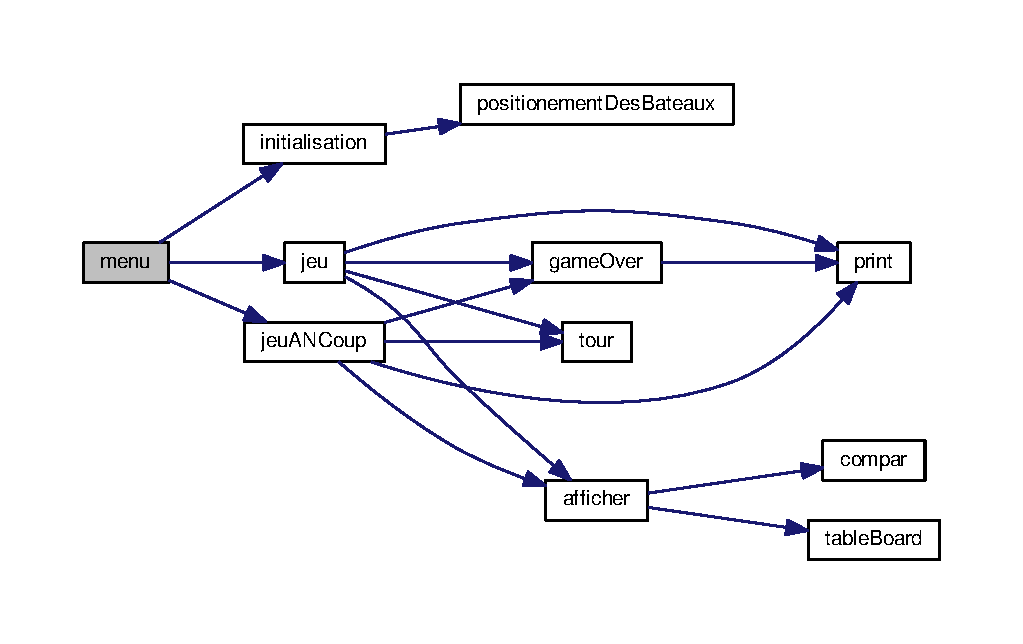
\includegraphics[width=350pt]{menu_8c_a2a0e843767aeea4f433a28b9c54f573a_cgraph}
\end{center}
\end{figure}
Voici le graphe des appelants de cette fonction \+:\nopagebreak
\begin{figure}[H]
\begin{center}
\leavevmode
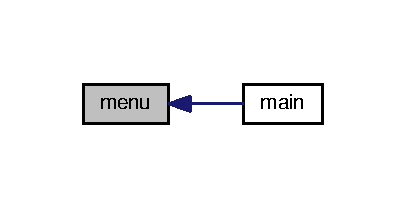
\includegraphics[width=195pt]{menu_8c_a2a0e843767aeea4f433a28b9c54f573a_icgraph}
\end{center}
\end{figure}

\hypertarget{positionnement_8c}{}\section{Référence du fichier positionnement.\+c}
\label{positionnement_8c}\index{positionnement.\+c@{positionnement.\+c}}
{\ttfamily \#include \char`\"{}header.\+h\char`\"{}}\newline
Graphe des dépendances par inclusion de positionnement.\+c\+:\nopagebreak
\begin{figure}[H]
\begin{center}
\leavevmode
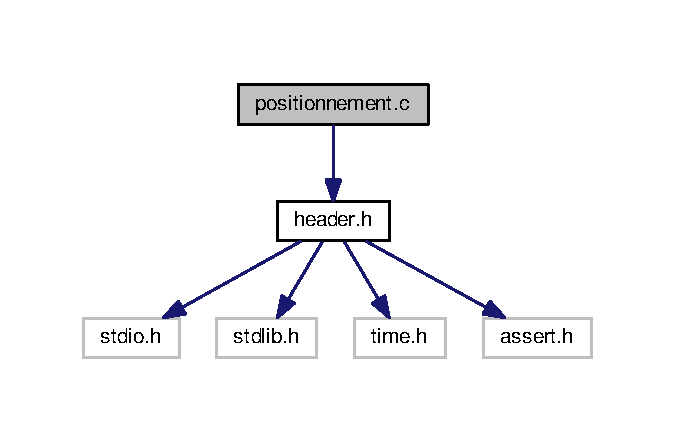
\includegraphics[width=324pt]{positionnement_8c__incl}
\end{center}
\end{figure}
\subsection*{Fonctions}
\begin{DoxyCompactItemize}
\item 
\mbox{\hyperlink{structjoueur}{joueur}} $\ast$ \mbox{\hyperlink{positionnement_8c_ad0373883ed5579d1c3a0dd93f257e558}{positionement\+Des\+Bateaux}} (\mbox{\hyperlink{structjoueur}{joueur}} $\ast$player)
\begin{DoxyCompactList}\small\item\em Une fonction qui posision les bateau de la bonne façon à chaque debut de jeu apres l\textquotesingle{}initialisation. \end{DoxyCompactList}\end{DoxyCompactItemize}


\subsection{Description détaillée}
\begin{DoxyAuthor}{Auteur}
B.\+Habib, A.\+Sofiane, I.\+Tinhinane, I.\+Chafia 
\end{DoxyAuthor}
\begin{DoxyVersion}{Version}
1.\+0 
\end{DoxyVersion}
\begin{DoxyDate}{Date}
07 Avril 2018
\end{DoxyDate}
définition de la fonction positionnement 

\subsection{Documentation des fonctions}
\mbox{\Hypertarget{positionnement_8c_ad0373883ed5579d1c3a0dd93f257e558}\label{positionnement_8c_ad0373883ed5579d1c3a0dd93f257e558}} 
\index{positionnement.\+c@{positionnement.\+c}!positionement\+Des\+Bateaux@{positionement\+Des\+Bateaux}}
\index{positionement\+Des\+Bateaux@{positionement\+Des\+Bateaux}!positionnement.\+c@{positionnement.\+c}}
\subsubsection{\texorpdfstring{positionement\+Des\+Bateaux()}{positionementDesBateaux()}}
{\footnotesize\ttfamily \mbox{\hyperlink{structjoueur}{joueur}}$\ast$ positionement\+Des\+Bateaux (\begin{DoxyParamCaption}\item[{\mbox{\hyperlink{structjoueur}{joueur}} $\ast$}]{player }\end{DoxyParamCaption})}



Une fonction qui posision les bateau de la bonne façon à chaque debut de jeu apres l\textquotesingle{}initialisation. 

Cette fonction permet de positionner les bateaux. 
\begin{DoxyParams}{Paramètres}
{\em joueur$\ast$} & player \+: le joueur concerner. \\
\hline
\end{DoxyParams}
\begin{DoxyReturn}{Renvoie}
Le joueur. 
\end{DoxyReturn}


Définition à la ligne 8 du fichier positionnement.\+c.



Références joueur\+::bat, bateau\+::color, bateau\+::nbr\+\_\+case\+\_\+colonne, bateau\+::nbr\+\_\+case\+\_\+ligne, bateau\+::nbr\+\_\+case\+\_\+total, bateau\+::nbr\+\_\+case\+\_\+toucher, N\+O\+M\+B\+R\+E\+\_\+\+B\+A\+T\+E\+AU, bateau\+::normale, joueur\+::plateau, bateau\+::position\+\_\+colonne, bateau\+::position\+\_\+ligne, T\+A\+I\+L\+L\+E\+\_\+\+P\+L\+A\+T\+E\+AU, et bateau\+::type.



Référencé par initialisation().


\begin{DoxyCode}
8                                                \{
9     \textcolor{keywordtype}{int} nbrCase = 2, occuper, choix1, choix2;
10     \textcolor{keywordtype}{int} posc, posl;
11     \textcolor{comment}{// Les 4 Bateaux sous forme de  ligne}
12     \textcolor{keywordflow}{for}(\textcolor{keywordtype}{int} i = 0; i < 4;i++)\{
13         player->\mbox{\hyperlink{structjoueur_a3b21aa14ce27f69126dc9a649b363146}{bat}}[i].\mbox{\hyperlink{structbateau_a1a56dd379e7c5cfc5714fd204947a0a8}{nbr\_case\_colonne}} = nbrCase++;
14         player->\mbox{\hyperlink{structjoueur_a3b21aa14ce27f69126dc9a649b363146}{bat}}[i].\mbox{\hyperlink{structbateau_a5f7637b2932717e5589e1a368dd1b47b}{nbr\_case\_ligne}} = 1;
15     \}
16     \textcolor{comment}{// Les Couleur donner pour chaque bateaux}
17     player->\mbox{\hyperlink{structjoueur_a3b21aa14ce27f69126dc9a649b363146}{bat}}[0].\mbox{\hyperlink{structbateau_a41910d4781ab6f3256d23f62b98c49a1}{color}} = \textcolor{stringliteral}{"32"};player->\mbox{\hyperlink{structjoueur_a3b21aa14ce27f69126dc9a649b363146}{bat}}[1].\mbox{\hyperlink{structbateau_a41910d4781ab6f3256d23f62b98c49a1}{color}} = \textcolor{stringliteral}{"33"};player->
      \mbox{\hyperlink{structjoueur_a3b21aa14ce27f69126dc9a649b363146}{bat}}[2].\mbox{\hyperlink{structbateau_a41910d4781ab6f3256d23f62b98c49a1}{color}} = \textcolor{stringliteral}{"34"};player->\mbox{\hyperlink{structjoueur_a3b21aa14ce27f69126dc9a649b363146}{bat}}[3].\mbox{\hyperlink{structbateau_a41910d4781ab6f3256d23f62b98c49a1}{color}} = \textcolor{stringliteral}{"35"};
18     player->\mbox{\hyperlink{structjoueur_a3b21aa14ce27f69126dc9a649b363146}{bat}}[4].\mbox{\hyperlink{structbateau_a41910d4781ab6f3256d23f62b98c49a1}{color}} = \textcolor{stringliteral}{"36"};player->\mbox{\hyperlink{structjoueur_a3b21aa14ce27f69126dc9a649b363146}{bat}}[5].\mbox{\hyperlink{structbateau_a41910d4781ab6f3256d23f62b98c49a1}{color}} = \textcolor{stringliteral}{"37"};player->
      \mbox{\hyperlink{structjoueur_a3b21aa14ce27f69126dc9a649b363146}{bat}}[6].\mbox{\hyperlink{structbateau_a41910d4781ab6f3256d23f62b98c49a1}{color}} = \textcolor{stringliteral}{"38"};player->\mbox{\hyperlink{structjoueur_a3b21aa14ce27f69126dc9a649b363146}{bat}}[7].\mbox{\hyperlink{structbateau_a41910d4781ab6f3256d23f62b98c49a1}{color}} = \textcolor{stringliteral}{"36"};
19     player->\mbox{\hyperlink{structjoueur_a3b21aa14ce27f69126dc9a649b363146}{bat}}[8].\mbox{\hyperlink{structbateau_a41910d4781ab6f3256d23f62b98c49a1}{color}} = \textcolor{stringliteral}{"32"};player->\mbox{\hyperlink{structjoueur_a3b21aa14ce27f69126dc9a649b363146}{bat}}[9].\mbox{\hyperlink{structbateau_a41910d4781ab6f3256d23f62b98c49a1}{color}} = \textcolor{stringliteral}{"33"};
20     \textcolor{comment}{// Les bateaux sous forme de 4x4 et 4x2}
21     player->\mbox{\hyperlink{structjoueur_a3b21aa14ce27f69126dc9a649b363146}{bat}}[4].\mbox{\hyperlink{structbateau_a1a56dd379e7c5cfc5714fd204947a0a8}{nbr\_case\_colonne}} = player->\mbox{\hyperlink{structjoueur_a3b21aa14ce27f69126dc9a649b363146}{bat}}[4].
      \mbox{\hyperlink{structbateau_a5f7637b2932717e5589e1a368dd1b47b}{nbr\_case\_ligne}} = 2;
22     player->\mbox{\hyperlink{structjoueur_a3b21aa14ce27f69126dc9a649b363146}{bat}}[5].\mbox{\hyperlink{structbateau_a1a56dd379e7c5cfc5714fd204947a0a8}{nbr\_case\_colonne}} = 4;player->\mbox{\hyperlink{structjoueur_a3b21aa14ce27f69126dc9a649b363146}{bat}}[5].
      \mbox{\hyperlink{structbateau_a5f7637b2932717e5589e1a368dd1b47b}{nbr\_case\_ligne}} = 2;
23     player->\mbox{\hyperlink{structjoueur_a3b21aa14ce27f69126dc9a649b363146}{bat}}[6].\mbox{\hyperlink{structbateau_a1a56dd379e7c5cfc5714fd204947a0a8}{nbr\_case\_colonne}} = player->\mbox{\hyperlink{structjoueur_a3b21aa14ce27f69126dc9a649b363146}{bat}}[6].
      \mbox{\hyperlink{structbateau_a5f7637b2932717e5589e1a368dd1b47b}{nbr\_case\_ligne}} = 4;
24     \textcolor{comment}{// on fait la déffirence  entre les bateaux normale(bateaux ligne, 4x4 et 4x2) est anormale(bateaux L,
       H et T)  }
25     \textcolor{keywordflow}{for} (\textcolor{keywordtype}{int} i = 0; i <= 6; ++i)\{   
26         player->\mbox{\hyperlink{structjoueur_a3b21aa14ce27f69126dc9a649b363146}{bat}}[i].\mbox{\hyperlink{structbateau_ac4078d21fa180ff7d5c7e7fbf8a4a773}{type}} = 0;\textcolor{comment}{// pour faire la deffirence entre les forme des bateaux}
27         player->\mbox{\hyperlink{structjoueur_a3b21aa14ce27f69126dc9a649b363146}{bat}}[i].\mbox{\hyperlink{structbateau_a77fe0bf7801ff08bf9b17e6c6237692e}{normale}} = 0;
28         player->\mbox{\hyperlink{structjoueur_a3b21aa14ce27f69126dc9a649b363146}{bat}}[i].\mbox{\hyperlink{structbateau_aff445dc58a52069759f1e4bfd13c0313}{nbr\_case\_total}} = player->\mbox{\hyperlink{structjoueur_a3b21aa14ce27f69126dc9a649b363146}{bat}}[i].
      \mbox{\hyperlink{structbateau_a5f7637b2932717e5589e1a368dd1b47b}{nbr\_case\_ligne}} * player->\mbox{\hyperlink{structjoueur_a3b21aa14ce27f69126dc9a649b363146}{bat}}[i].\mbox{\hyperlink{structbateau_a1a56dd379e7c5cfc5714fd204947a0a8}{nbr\_case\_colonne}};\textcolor{comment}{// Nombre total de case
       pour chaque  bateau}
29     \}
30     \textcolor{comment}{// Les bateau sous forme de L, H et T}
31     player->\mbox{\hyperlink{structjoueur_a3b21aa14ce27f69126dc9a649b363146}{bat}}[7].\mbox{\hyperlink{structbateau_a1a56dd379e7c5cfc5714fd204947a0a8}{nbr\_case\_colonne}} = player->\mbox{\hyperlink{structjoueur_a3b21aa14ce27f69126dc9a649b363146}{bat}}[7].
      \mbox{\hyperlink{structbateau_a5f7637b2932717e5589e1a368dd1b47b}{nbr\_case\_ligne}} = 4; player->\mbox{\hyperlink{structjoueur_a3b21aa14ce27f69126dc9a649b363146}{bat}}[7].\mbox{\hyperlink{structbateau_a77fe0bf7801ff08bf9b17e6c6237692e}{normale}} = 1; player->
      \mbox{\hyperlink{structjoueur_a3b21aa14ce27f69126dc9a649b363146}{bat}}[7].\mbox{\hyperlink{structbateau_ac4078d21fa180ff7d5c7e7fbf8a4a773}{type}} = 1; player->\mbox{\hyperlink{structjoueur_a3b21aa14ce27f69126dc9a649b363146}{bat}}[7].\mbox{\hyperlink{structbateau_aff445dc58a52069759f1e4bfd13c0313}{nbr\_case\_total}} = 7;
32     player->\mbox{\hyperlink{structjoueur_a3b21aa14ce27f69126dc9a649b363146}{bat}}[8].\mbox{\hyperlink{structbateau_a1a56dd379e7c5cfc5714fd204947a0a8}{nbr\_case\_colonne}} = 3; player->\mbox{\hyperlink{structjoueur_a3b21aa14ce27f69126dc9a649b363146}{bat}}[8].
      \mbox{\hyperlink{structbateau_a5f7637b2932717e5589e1a368dd1b47b}{nbr\_case\_ligne}} = 4; player->\mbox{\hyperlink{structjoueur_a3b21aa14ce27f69126dc9a649b363146}{bat}}[8].\mbox{\hyperlink{structbateau_a77fe0bf7801ff08bf9b17e6c6237692e}{normale}} = 1; player->
      \mbox{\hyperlink{structjoueur_a3b21aa14ce27f69126dc9a649b363146}{bat}}[8].\mbox{\hyperlink{structbateau_ac4078d21fa180ff7d5c7e7fbf8a4a773}{type}} = 2; player->\mbox{\hyperlink{structjoueur_a3b21aa14ce27f69126dc9a649b363146}{bat}}[8].\mbox{\hyperlink{structbateau_aff445dc58a52069759f1e4bfd13c0313}{nbr\_case\_total}} = 6;
33     player->\mbox{\hyperlink{structjoueur_a3b21aa14ce27f69126dc9a649b363146}{bat}}[9].\mbox{\hyperlink{structbateau_a1a56dd379e7c5cfc5714fd204947a0a8}{nbr\_case\_colonne}} = player->\mbox{\hyperlink{structjoueur_a3b21aa14ce27f69126dc9a649b363146}{bat}}[9].
      \mbox{\hyperlink{structbateau_a5f7637b2932717e5589e1a368dd1b47b}{nbr\_case\_ligne}} = 3; player->\mbox{\hyperlink{structjoueur_a3b21aa14ce27f69126dc9a649b363146}{bat}}[9].\mbox{\hyperlink{structbateau_a77fe0bf7801ff08bf9b17e6c6237692e}{normale}} = 1; player->
      \mbox{\hyperlink{structjoueur_a3b21aa14ce27f69126dc9a649b363146}{bat}}[9].\mbox{\hyperlink{structbateau_ac4078d21fa180ff7d5c7e7fbf8a4a773}{type}} = 3; player->\mbox{\hyperlink{structjoueur_a3b21aa14ce27f69126dc9a649b363146}{bat}}[9].\mbox{\hyperlink{structbateau_aff445dc58a52069759f1e4bfd13c0313}{nbr\_case\_total}} = 7;
34     \textcolor{comment}{// Placement des Bateaux dans le plateau}
35     \textcolor{keywordflow}{for}(\textcolor{keywordtype}{int} i = 0 ; i < \mbox{\hyperlink{header_8h_a56aaacd8cb8ffd138094887b2d3344f6}{NOMBRE\_BATEAU}} ; i++)\{
36         player->\mbox{\hyperlink{structjoueur_a3b21aa14ce27f69126dc9a649b363146}{bat}}[i].\mbox{\hyperlink{structbateau_a62ae80832c521a9984c520fde88dadfd}{nbr\_case\_toucher}} = 0;\textcolor{comment}{// Au debut aucune case n'est toucher }
37         \textcolor{comment}{//chercher une bonne position pour chaque bateau}
38         \textcolor{keywordflow}{do}\{
39             occuper = 0;
40             posc = rand() \% (\mbox{\hyperlink{header_8h_adc3c2556e84bebbe78c8a87fc459a6f8}{TAILLE\_PLATEAU}} - player->\mbox{\hyperlink{structjoueur_a3b21aa14ce27f69126dc9a649b363146}{bat}}[i].
      \mbox{\hyperlink{structbateau_a1a56dd379e7c5cfc5714fd204947a0a8}{nbr\_case\_colonne}} + 1);\textcolor{comment}{// Colonne de positionement du bateau}
41             posl = rand() \% (\mbox{\hyperlink{header_8h_adc3c2556e84bebbe78c8a87fc459a6f8}{TAILLE\_PLATEAU}} - player->\mbox{\hyperlink{structjoueur_a3b21aa14ce27f69126dc9a649b363146}{bat}}[i].
      \mbox{\hyperlink{structbateau_a5f7637b2932717e5589e1a368dd1b47b}{nbr\_case\_ligne}} + 1); \textcolor{comment}{// Ligne de positionement du bateau}
42             \textcolor{comment}{//printf("posl = \%d   posc = \%d \(\backslash\)n",posl,posc);}
43             \textcolor{comment}{// Vérifié si il y n'a pas un autre bateau sur cette position}
44             \textcolor{keywordflow}{for}(\textcolor{keywordtype}{int} j = posl ; j < posl + player->\mbox{\hyperlink{structjoueur_a3b21aa14ce27f69126dc9a649b363146}{bat}}[i].\mbox{\hyperlink{structbateau_a5f7637b2932717e5589e1a368dd1b47b}{nbr\_case\_ligne}} ; j++)\{
45                 \textcolor{keywordflow}{for}(\textcolor{keywordtype}{int} k = posc ; k < posc + player->\mbox{\hyperlink{structjoueur_a3b21aa14ce27f69126dc9a649b363146}{bat}}[i].\mbox{\hyperlink{structbateau_a1a56dd379e7c5cfc5714fd204947a0a8}{nbr\_case\_colonne}} ; ++k)\{
46                     \textcolor{keywordflow}{if}(player->\mbox{\hyperlink{structjoueur_a0de66c3578a57ff8e0ed1bf3d91c8e82}{plateau}}[j][k] == \textcolor{charliteral}{'\#'})\{
47                         occuper = 1;
48                         \textcolor{keywordflow}{break};
49                     \}
50                 \}   
51                 \textcolor{keywordflow}{if}(occuper == 1)\textcolor{keywordflow}{break};
52             \}
53             \textcolor{keywordflow}{if}(player->\mbox{\hyperlink{structjoueur_a3b21aa14ce27f69126dc9a649b363146}{bat}}[i].\mbox{\hyperlink{structbateau_a77fe0bf7801ff08bf9b17e6c6237692e}{normale}})\{
54                 \textcolor{keywordflow}{for} (\textcolor{keywordtype}{int} j = 0; j < i; ++j)\{
55                     \textcolor{keywordflow}{if}(((posc >= player-> \mbox{\hyperlink{structjoueur_a3b21aa14ce27f69126dc9a649b363146}{bat}}[i].\mbox{\hyperlink{structbateau_aac775edde7cde57176e580c29f6e8eca}{position\_colonne}})
56                             \&\& (posc < player-> \mbox{\hyperlink{structjoueur_a3b21aa14ce27f69126dc9a649b363146}{bat}}[j].\mbox{\hyperlink{structbateau_aac775edde7cde57176e580c29f6e8eca}{position\_colonne}} + player-> 
      \mbox{\hyperlink{structjoueur_a3b21aa14ce27f69126dc9a649b363146}{bat}}[j].\mbox{\hyperlink{structbateau_a1a56dd379e7c5cfc5714fd204947a0a8}{nbr\_case\_colonne}})) \&\&
57                             ((posl >= player-> \mbox{\hyperlink{structjoueur_a3b21aa14ce27f69126dc9a649b363146}{bat}}[j].\mbox{\hyperlink{structbateau_a5dcd33e534b9b1b8b0414325bc5c09b1}{position\_ligne}})
58                             \&\& (posl < player-> \mbox{\hyperlink{structjoueur_a3b21aa14ce27f69126dc9a649b363146}{bat}}[j].position\_ligne + player-> 
      \mbox{\hyperlink{structjoueur_a3b21aa14ce27f69126dc9a649b363146}{bat}}[j].\mbox{\hyperlink{structbateau_a5f7637b2932717e5589e1a368dd1b47b}{nbr\_case\_ligne}})))\{
59                         occuper = 1;
60                         \textcolor{keywordflow}{break};
61                     \}
62                 \}
63             \}
64         \} \textcolor{keywordflow}{while} (occuper == 1);\textcolor{comment}{// repeter tanque il y déja un bateau sur cette position }
65         \textcolor{comment}{//Affecter la bonne position au bateau }
66         player->\mbox{\hyperlink{structjoueur_a3b21aa14ce27f69126dc9a649b363146}{bat}}[i].\mbox{\hyperlink{structbateau_a5dcd33e534b9b1b8b0414325bc5c09b1}{position\_ligne}} = posl; 
67         player->\mbox{\hyperlink{structjoueur_a3b21aa14ce27f69126dc9a649b363146}{bat}}[i].\mbox{\hyperlink{structbateau_aac775edde7cde57176e580c29f6e8eca}{position\_colonne}} = posc;
68         \textcolor{comment}{// Dessiner le bateau selon sa forme (ligne, 4x4, 4x2, L, H et T ...)}
69         \textcolor{keywordflow}{if}(player->\mbox{\hyperlink{structjoueur_a3b21aa14ce27f69126dc9a649b363146}{bat}}[i].\mbox{\hyperlink{structbateau_a77fe0bf7801ff08bf9b17e6c6237692e}{normale}} == 0)\{
70             \textcolor{keywordflow}{for}(\textcolor{keywordtype}{int} j = posl ; j < posl + player->\mbox{\hyperlink{structjoueur_a3b21aa14ce27f69126dc9a649b363146}{bat}}[i].\mbox{\hyperlink{structbateau_a5f7637b2932717e5589e1a368dd1b47b}{nbr\_case\_ligne}} ; j++)
71                 \textcolor{keywordflow}{for}(\textcolor{keywordtype}{int} k = posc ; k < posc + player->\mbox{\hyperlink{structjoueur_a3b21aa14ce27f69126dc9a649b363146}{bat}}[i].\mbox{\hyperlink{structbateau_a1a56dd379e7c5cfc5714fd204947a0a8}{nbr\_case\_colonne}} ; ++k)
72                     player->\mbox{\hyperlink{structjoueur_a0de66c3578a57ff8e0ed1bf3d91c8e82}{plateau}}[j][k] = \textcolor{charliteral}{'\#'};
73         \}\textcolor{keywordflow}{else}\{
74             \textcolor{keywordflow}{switch} (player->\mbox{\hyperlink{structjoueur_a3b21aa14ce27f69126dc9a649b363146}{bat}}[i].\mbox{\hyperlink{structbateau_ac4078d21fa180ff7d5c7e7fbf8a4a773}{type}})\{
75                 \textcolor{keywordflow}{case} 1 :\{\textcolor{comment}{// Bateau sous forme de L 4 cas}
76                     choix1 = rand()\%3 + 1;
77                     choix2 = rand()\%3 + 1;
78                     \textcolor{keywordflow}{if}(choix2 == 2 ) choix2 = posl + player->\mbox{\hyperlink{structjoueur_a3b21aa14ce27f69126dc9a649b363146}{bat}}[i].
      \mbox{\hyperlink{structbateau_a5f7637b2932717e5589e1a368dd1b47b}{nbr\_case\_ligne}} - 1 ;
79                     \textcolor{keywordflow}{else} choix2 = posl ;
80 
81                     \textcolor{keywordflow}{if}(choix1 == 2 ) choix1 = posc + player->\mbox{\hyperlink{structjoueur_a3b21aa14ce27f69126dc9a649b363146}{bat}}[i].
      \mbox{\hyperlink{structbateau_a1a56dd379e7c5cfc5714fd204947a0a8}{nbr\_case\_colonne}} - 1 ;
82                     \textcolor{keywordflow}{else} choix1 = posc ;
83                 \}
84                 \textcolor{keywordflow}{break};
85                 \textcolor{keywordflow}{case} 2 :\{\textcolor{comment}{// Bateau sous forme de T}
86                     choix1 = posc + player->\mbox{\hyperlink{structjoueur_a3b21aa14ce27f69126dc9a649b363146}{bat}}[i].\mbox{\hyperlink{structbateau_a1a56dd379e7c5cfc5714fd204947a0a8}{nbr\_case\_colonne}}/2;
87                     choix2 = posl;
88                 \}
89                 \textcolor{keywordflow}{break};
90                 \textcolor{keywordflow}{case} 3 :\{\textcolor{comment}{// Bateau sous forme de H}
91                     choix1 = posc + player->\mbox{\hyperlink{structjoueur_a3b21aa14ce27f69126dc9a649b363146}{bat}}[i].\mbox{\hyperlink{structbateau_a1a56dd379e7c5cfc5714fd204947a0a8}{nbr\_case\_colonne}} - 1;
92                     choix2 = posl + player->\mbox{\hyperlink{structjoueur_a3b21aa14ce27f69126dc9a649b363146}{bat}}[i].\mbox{\hyperlink{structbateau_a5f7637b2932717e5589e1a368dd1b47b}{nbr\_case\_ligne}} / 2;
93                 \}
94                 \textcolor{keywordflow}{break};
95             \}
96             \textcolor{comment}{// Placer les bateaux dans le plateau }
97             \textcolor{keywordflow}{for}(\textcolor{keywordtype}{int} j = posl ; j < posl + player->\mbox{\hyperlink{structjoueur_a3b21aa14ce27f69126dc9a649b363146}{bat}}[i].\mbox{\hyperlink{structbateau_a5f7637b2932717e5589e1a368dd1b47b}{nbr\_case\_ligne}} ; j++)
98                 player->\mbox{\hyperlink{structjoueur_a0de66c3578a57ff8e0ed1bf3d91c8e82}{plateau}}[j][choix1] = \textcolor{charliteral}{'\#'};
99 
100             \textcolor{keywordflow}{if}(player->\mbox{\hyperlink{structjoueur_a3b21aa14ce27f69126dc9a649b363146}{bat}}[i].\mbox{\hyperlink{structbateau_ac4078d21fa180ff7d5c7e7fbf8a4a773}{type}} == 3)\{
101                 \textcolor{keywordflow}{for}(\textcolor{keywordtype}{int} j = posl ; j < posl + player->\mbox{\hyperlink{structjoueur_a3b21aa14ce27f69126dc9a649b363146}{bat}}[i].\mbox{\hyperlink{structbateau_a5f7637b2932717e5589e1a368dd1b47b}{nbr\_case\_ligne}} ; j++)
102                 player->\mbox{\hyperlink{structjoueur_a0de66c3578a57ff8e0ed1bf3d91c8e82}{plateau}}[j][posc] = \textcolor{charliteral}{'\#'};
103             \}
104 
105             \textcolor{keywordflow}{for}(\textcolor{keywordtype}{int} k = posc ; k < posc + player->\mbox{\hyperlink{structjoueur_a3b21aa14ce27f69126dc9a649b363146}{bat}}[i].\mbox{\hyperlink{structbateau_a1a56dd379e7c5cfc5714fd204947a0a8}{nbr\_case\_colonne}} ; ++k) 
106                 player->\mbox{\hyperlink{structjoueur_a0de66c3578a57ff8e0ed1bf3d91c8e82}{plateau}}[choix2][k] = \textcolor{charliteral}{'\#'};
107         \}
108     \}
109 
110 \textcolor{keywordflow}{return} player;
111 \}
\end{DoxyCode}
Voici le graphe des appelants de cette fonction \+:\nopagebreak
\begin{figure}[H]
\begin{center}
\leavevmode
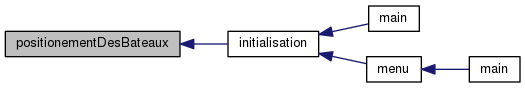
\includegraphics[width=350pt]{positionnement_8c_ad0373883ed5579d1c3a0dd93f257e558_icgraph}
\end{center}
\end{figure}

\hypertarget{tester_8c}{}\section{Référence du fichier tester.\+c}
\label{tester_8c}\index{tester.\+c@{tester.\+c}}
{\ttfamily \#include \char`\"{}header.\+h\char`\"{}}\newline
Graphe des dépendances par inclusion de tester.\+c\+:\nopagebreak
\begin{figure}[H]
\begin{center}
\leavevmode
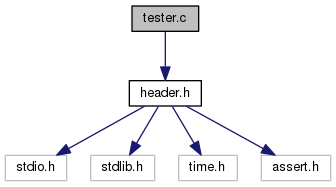
\includegraphics[width=324pt]{tester_8c__incl}
\end{center}
\end{figure}
\subsection*{Fonctions}
\begin{DoxyCompactItemize}
\item 
int \mbox{\hyperlink{tester_8c_a840291bc02cba5474a4cb46a9b9566fe}{main}} (void)
\end{DoxyCompactItemize}


\subsection{Documentation des fonctions}
\mbox{\Hypertarget{tester_8c_a840291bc02cba5474a4cb46a9b9566fe}\label{tester_8c_a840291bc02cba5474a4cb46a9b9566fe}} 
\index{tester.\+c@{tester.\+c}!main@{main}}
\index{main@{main}!tester.\+c@{tester.\+c}}
\subsubsection{\texorpdfstring{main()}{main()}}
{\footnotesize\ttfamily int main (\begin{DoxyParamCaption}\item[{void}]{ }\end{DoxyParamCaption})}



Définition à la ligne 4 du fichier tester.\+c.



Références game\+Over(), G\+R\+E\+EN, initialisation(), tour(), et Y\+E\+L\+L\+OW.


\begin{DoxyCode}
4                 \{
5   \textcolor{keywordflow}{for}(\textcolor{keywordtype}{int} i = 1; i< 100;i++)\{
6   printf (\textcolor{stringliteral}{"Debut des tests\(\backslash\)n"});
7   
8   \mbox{\hyperlink{structjoueur}{joueur}}* player1 = NULL;
9   player1 = \mbox{\hyperlink{header_8h_aa69260c04e3640b56e402f842f5b7448}{initialisation}}(player1,\mbox{\hyperlink{header_8h_acfbc006ea433ad708fdee3e82996e721}{GREEN}},1);
10   assert (player1 != NULL);
11 
12   \mbox{\hyperlink{structjoueur}{joueur}}* player2 = NULL;
13   player2 = \mbox{\hyperlink{header_8h_aa69260c04e3640b56e402f842f5b7448}{initialisation}}(player2,\mbox{\hyperlink{header_8h_abf681265909adf3d3e8116c93c0ba179}{YELLOW}},1);
14   assert (player2 != NULL);
15   
16   \mbox{\hyperlink{structjoueur}{joueur}}* joueurActualle = player1;
17   \textcolor{keywordflow}{while}(!\mbox{\hyperlink{header_8h_a3106323267d0c2e16a73616d1666831a}{gameOver}}(joueurActualle))\{
18 
19     joueurActualle = player1;
20     player2 = \mbox{\hyperlink{header_8h_a92241da559f8c98b3ec5a99f4d151658}{tour}}(player1, player2);
21 
22     \textcolor{keywordflow}{if}(!\mbox{\hyperlink{header_8h_a3106323267d0c2e16a73616d1666831a}{gameOver}}(joueurActualle))\{
23 
24       joueurActualle = player2;
25       player1 = \mbox{\hyperlink{header_8h_a92241da559f8c98b3ec5a99f4d151658}{tour}}(player2, player1);      
26     \}\textcolor{keywordflow}{else}\{
27       \textcolor{keywordflow}{break};
28     \}
29   \}
30   printf(\textcolor{stringliteral}{"\(\backslash\)n-------------------------------\(\backslash\)n"});
31   \}
32   printf (\textcolor{stringliteral}{"Tout est OK\(\backslash\)n"});
33 
34   \textcolor{keywordflow}{return} (EXIT\_SUCCESS);
35 \}
\end{DoxyCode}
Voici le graphe d\textquotesingle{}appel pour cette fonction \+:\nopagebreak
\begin{figure}[H]
\begin{center}
\leavevmode
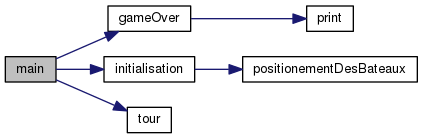
\includegraphics[width=350pt]{tester_8c_a840291bc02cba5474a4cb46a9b9566fe_cgraph}
\end{center}
\end{figure}

\hypertarget{tour_8c}{}\section{Référence du fichier tour.\+c}
\label{tour_8c}\index{tour.\+c@{tour.\+c}}
{\ttfamily \#include \char`\"{}header.\+h\char`\"{}}\newline
Graphe des dépendances par inclusion de tour.\+c\+:\nopagebreak
\begin{figure}[H]
\begin{center}
\leavevmode
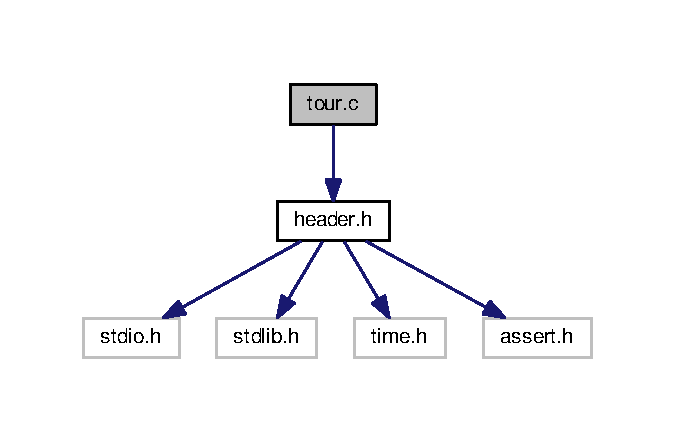
\includegraphics[width=324pt]{tour_8c__incl}
\end{center}
\end{figure}
\subsection*{Fonctions}
\begin{DoxyCompactItemize}
\item 
\mbox{\hyperlink{structjoueur}{joueur}} $\ast$ \mbox{\hyperlink{tour_8c_aadff1874927a9be4d824b9b291457d7d}{tour}} (\mbox{\hyperlink{structjoueur}{joueur}} $\ast$player1, \mbox{\hyperlink{structjoueur}{joueur}} $\ast$player2)
\begin{DoxyCompactList}\small\item\em Une fonction qui déroule le tour d\textquotesingle{}un jour. \end{DoxyCompactList}\end{DoxyCompactItemize}


\subsection{Documentation des fonctions}
\mbox{\Hypertarget{tour_8c_aadff1874927a9be4d824b9b291457d7d}\label{tour_8c_aadff1874927a9be4d824b9b291457d7d}} 
\index{tour.\+c@{tour.\+c}!tour@{tour}}
\index{tour@{tour}!tour.\+c@{tour.\+c}}
\subsubsection{\texorpdfstring{tour()}{tour()}}
{\footnotesize\ttfamily \mbox{\hyperlink{structjoueur}{joueur}}$\ast$ tour (\begin{DoxyParamCaption}\item[{\mbox{\hyperlink{structjoueur}{joueur}} $\ast$}]{player1,  }\item[{\mbox{\hyperlink{structjoueur}{joueur}} $\ast$}]{player2 }\end{DoxyParamCaption})}



Une fonction qui déroule le tour d\textquotesingle{}un jour. 

Cette fonction permet de jouer un tour. 
\begin{DoxyParams}{Paramètres}
{\em joueur$\ast$} & player1 \+: le joueur qui joue ~\newline
\\
\hline
{\em joueur$\ast$} & player2 \+: le joueur l\textquotesingle{}adversaire. ~\newline
\\
\hline
\end{DoxyParams}
\begin{DoxyReturn}{Renvoie}
Le joueur. 
\end{DoxyReturn}


Définition à la ligne 10 du fichier tour.\+c.



Références joueur\+::bat, joueur\+::ia, bateau\+::nbr\+\_\+case\+\_\+colonne, bateau\+::nbr\+\_\+case\+\_\+ligne, bateau\+::nbr\+\_\+case\+\_\+toucher, joueur\+::nbr\+\_\+tir\+\_\+manquer, joueur\+::nbr\+\_\+tir\+\_\+reussit, N\+O\+M\+B\+R\+E\+\_\+\+B\+A\+T\+E\+AU, joueur\+::plateau, bateau\+::position\+\_\+colonne, bateau\+::position\+\_\+ligne, et T\+A\+I\+L\+L\+E\+\_\+\+P\+L\+A\+T\+E\+AU.



Référencé par jeu(), jeu\+A\+N\+Coup(), et main().


\begin{DoxyCode}
10                                               \{
11   \textcolor{keywordtype}{int} ligne,colonne,occuper,i;
12 
13   \textcolor{keywordflow}{do}\{
14     occuper = 0;
15     \textcolor{comment}{// Obtenir le choix du joueur1 pour attaque une case  }
16     \textcolor{keywordflow}{if}(!player1->\mbox{\hyperlink{structjoueur_a307e3b4b4c1b78e753c599bc1f6a47c3}{ia}})\{
17       \textcolor{comment}{// Si le joueur1 est un humaine}
18       \textcolor{keywordflow}{do}\{
19           printf(\textcolor{stringliteral}{"(ligne,colonne) :"});
20           scanf(\textcolor{stringliteral}{"\%d \%d"},\&ligne,\&colonne);
21       \}\textcolor{keywordflow}{while}((ligne > \mbox{\hyperlink{header_8h_adc3c2556e84bebbe78c8a87fc459a6f8}{TAILLE\_PLATEAU}} || ligne < 0) || (colonne > 
      \mbox{\hyperlink{header_8h_adc3c2556e84bebbe78c8a87fc459a6f8}{TAILLE\_PLATEAU}} || colonne < 0));
22     \}\textcolor{keywordflow}{else}\{
23       \textcolor{comment}{// Si le joueur1 est une IA}
24       ligne = rand()\%\mbox{\hyperlink{header_8h_adc3c2556e84bebbe78c8a87fc459a6f8}{TAILLE\_PLATEAU}} + 1;
25       colonne = rand()\%\mbox{\hyperlink{header_8h_adc3c2556e84bebbe78c8a87fc459a6f8}{TAILLE\_PLATEAU}} + 1;
26     \}
27     \textcolor{comment}{// Savoir quelle case est touché celle d'un bateau ou une case vide ou une deja joue précdament }
28     \textcolor{keywordflow}{if}(player2->\mbox{\hyperlink{structjoueur_a0de66c3578a57ff8e0ed1bf3d91c8e82}{plateau}}[ligne - 1][colonne - 1] == \textcolor{charliteral}{'\#'})\{
29       \textcolor{comment}{//bateau toucher incrémentation du nombre de tire réussi}
30       player2->\mbox{\hyperlink{structjoueur_a0de66c3578a57ff8e0ed1bf3d91c8e82}{plateau}}[ligne - 1][colonne - 1] = \textcolor{charliteral}{'X'};
31       player1->\mbox{\hyperlink{structjoueur_a19510a02b4ff3f6336da487b50806d71}{nbr\_tir\_reussit}}++;
32       \textcolor{comment}{// Savoir quelle bateau est toucher est incrémenter le nombre de case toucher pour ce bateau }
33       \textcolor{keywordflow}{for} (i = 0; i < \mbox{\hyperlink{header_8h_a56aaacd8cb8ffd138094887b2d3344f6}{NOMBRE\_BATEAU}}; ++i)\{
34         \textcolor{keywordflow}{if}(((colonne - 1 >= player2-> \mbox{\hyperlink{structjoueur_a3b21aa14ce27f69126dc9a649b363146}{bat}}[i].\mbox{\hyperlink{structbateau_aac775edde7cde57176e580c29f6e8eca}{position\_colonne}})
35             \&\& (colonne - 1 < player2-> \mbox{\hyperlink{structjoueur_a3b21aa14ce27f69126dc9a649b363146}{bat}}[i].\mbox{\hyperlink{structbateau_aac775edde7cde57176e580c29f6e8eca}{position\_colonne}} + player2-> 
      \mbox{\hyperlink{structjoueur_a3b21aa14ce27f69126dc9a649b363146}{bat}}[i].\mbox{\hyperlink{structbateau_a1a56dd379e7c5cfc5714fd204947a0a8}{nbr\_case\_colonne}})) \&\&
36             ((ligne - 1 >= player2-> \mbox{\hyperlink{structjoueur_a3b21aa14ce27f69126dc9a649b363146}{bat}}[i].\mbox{\hyperlink{structbateau_a5dcd33e534b9b1b8b0414325bc5c09b1}{position\_ligne}})
37             \&\& (ligne  - 1< player2-> \mbox{\hyperlink{structjoueur_a3b21aa14ce27f69126dc9a649b363146}{bat}}[i].\mbox{\hyperlink{structbateau_a5dcd33e534b9b1b8b0414325bc5c09b1}{position\_ligne}} + player2->
      \mbox{\hyperlink{structjoueur_a3b21aa14ce27f69126dc9a649b363146}{bat}}[i].\mbox{\hyperlink{structbateau_a5f7637b2932717e5589e1a368dd1b47b}{nbr\_case\_ligne}})))\{
38           player2->\mbox{\hyperlink{structjoueur_a3b21aa14ce27f69126dc9a649b363146}{bat}}[i].\mbox{\hyperlink{structbateau_a62ae80832c521a9984c520fde88dadfd}{nbr\_case\_toucher}}++;
39           \textcolor{keywordflow}{break};
40         \}
41       \}
42     \}
43     \textcolor{keywordflow}{else}\{
44       \textcolor{keywordflow}{if} (player2->\mbox{\hyperlink{structjoueur_a0de66c3578a57ff8e0ed1bf3d91c8e82}{plateau}}[ligne - 1][colonne - 1] == \textcolor{charliteral}{'X'} || player2->
      \mbox{\hyperlink{structjoueur_a0de66c3578a57ff8e0ed1bf3d91c8e82}{plateau}}[ligne - 1][colonne - 1] == \textcolor{charliteral}{'O'} )
45         occuper = 1;\textcolor{comment}{// Case précédament toucher }
46       \textcolor{keywordflow}{else}\{
47         \textcolor{comment}{// case vide toucher incréménter le nombre de tir manger}
48         player2->\mbox{\hyperlink{structjoueur_a0de66c3578a57ff8e0ed1bf3d91c8e82}{plateau}}[ligne - 1][colonne - 1] = \textcolor{charliteral}{'O'};
49         player1->\mbox{\hyperlink{structjoueur_aaba095a23d03a15d363924e77caa3c1e}{nbr\_tir\_manquer}}++;
50       \}
51     \}
52   \}\textcolor{keywordflow}{while}(occuper == 1);
53 
54   \textcolor{keywordflow}{return} player2;
55 \}
\end{DoxyCode}
Voici le graphe des appelants de cette fonction \+:\nopagebreak
\begin{figure}[H]
\begin{center}
\leavevmode
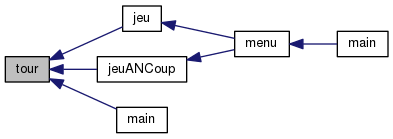
\includegraphics[width=350pt]{tour_8c_aadff1874927a9be4d824b9b291457d7d_icgraph}
\end{center}
\end{figure}

%--- End generated contents ---

% Index
\backmatter
\newpage
\phantomsection
\clearemptydoublepage
\addcontentsline{toc}{chapter}{Index}
\printindex

\end{document}
